\documentclass{uetgraduation}

% --- Các gói hỗ trợ toán học và bảng biểu nâng cao ---
\usepackage{amssymb}
\usepackage{booktabs}
\usepackage{multirow}
\usepackage{tabularx}
\usepackage{array}
\usepackage{longtable}
\usepackage[section]{placeins}

% --- Thuật toán giả định dạng tiếng Việt ---
\usepackage[linesnumbered,ruled,vlined]{algorithm2e}
\SetKwInput{KwIn}{Dữ liệu vào}
\SetKwInput{KwOut}{Kết quả}
\SetKw{KwTo}{đến}

% --- Cấu hình liên kết và đánh dấu Bookmarks ---
\usepackage{hyperref}
\hypersetup{
    colorlinks=true,
    linkcolor=black,
    citecolor=blue,
    urlcolor=blue,
    pdfauthor={Nguyễn Anh Sơn},
    pdftitle={Nghiên cứu khung học máy cho dự đoán mức độ triệu chứng trầm cảm từ dữ liệu sinh lý (DepSev-ML)},
    pdfsubject={Khóa luận tốt nghiệp đại học hệ chính quy},
    pdfkeywords={DepSev-ML, PHQ-9, Machine Learning, NHANES, Depression Severity}
}

\begin{document}

% ==================== THÔNG TIN BÌA VÀ PHỤ BÌA (CHUẨN VNU-UET) ====================
\studentname{Nguyễn Anh Sơn}
\title{Nghiên cứu khung học máy cho dự đoán mức độ triệu chứng trầm cảm từ dữ liệu sinh lý (DepSev-ML)}
\documenttype{Khóa luận tốt nghiệp đại học hệ chính quy}
\major{Công nghệ thông tin}
\year{2026}
\supervisor{Cán bộ Hướng dẫn Khoa học}
\englishtitle{A Machine Learning Framework for Depression Severity Prediction from Physiological Data (DepSev-ML)}
\englishmajor{Information Technology}
\englishsupervisor{Academic Supervisor}

% Khởi tạo các trang bìa chính, bìa phụ tiếng Việt và bìa phụ tiếng Anh
\makecovers

% Bật đánh số trang từ phần Preamble
\pagestyle{plain}

% ==================== PHẦN MỞ ĐẦU (PREAMBLE) ====================
\begin{preamble}{Lời cảm ơn}
Lời mở đầu, tôi xin gửi lời cảm ơn chân thành và sâu sắc nhất đến Cán bộ Hướng dẫn khoa học, Trường Đại học Công nghệ -- Đại học Quốc gia Hà Nội. Sự chỉ dẫn tận tình, những định hướng học thuật chuẩn xác, cùng với sự khắt khe về tính liêm chính khoa học và phương pháp luận nghiên cứu từ Cán bộ Hướng dẫn đã giúp tôi vượt qua nhiều thử thách để hoàn thành công trình nghiên cứu này.

Tôi cũng xin bày tỏ lòng biết ơn chân thành đến các Thầy, Cô giáo tại Khoa Công nghệ Thông tin, Trường Đại học Công nghệ -- Đại học Quốc gia Hà Nội, những người đã truyền dạy cho tôi nền tảng tri thức vững chắc về khoa học máy tính, học máy và kỹ thuật dữ liệu trong suốt quá trình học tập và nghiên cứu tại trường.

Đồng thời, tôi xin gửi lời cảm ơn chân thành đến Trung tâm Thống kê Y tế Quốc gia Hoa Kỳ (NCHS) thuộc Trung tâm Kiểm soát và Phòng ngừa Dịch bệnh (CDC) đã công khai bộ dữ liệu Khảo sát Kiểm tra Sức khỏe và Dinh dưỡng Quốc gia (NHANES), tạo tiền đề dữ liệu thực nghiệm quý báu cho đề tài.

Cuối cùng, tôi xin gửi lời tri ân sâu sắc đến gia đình, người thân và bạn bè -- những người luôn là điểm tựa tinh thần vững chắc, luôn đồng hành, động viên và chia sẻ với tôi trong suốt thời gian qua.

Mặc dù đã nỗ lực hết mình với tinh thần nghiên cứu nghiêm túc, nhưng do tính chất phức tạp của bài toán dự đoán sức khỏe tâm thần từ dữ liệu đa chiều, báo cáo khó tránh khỏi những hạn chế nhất định. Tôi rất mong nhận được những ý kiến đóng góp quý báu từ quý Thầy, Cô và Hội đồng chuyên môn để nghiên cứu được hoàn thiện hơn nữa.

\vspace{1.5cm}
\begin{flushright}
\textit{Hà Nội, năm 2026}\\[0.2cm]
\textbf{Sinh viên thực hiện}\\[1.5cm]
\textbf{Nguyễn Anh Sơn}
\end{flushright}
\end{preamble}

\begin{preamble}{Lời cam đoan}
Tôi xin cam đoan rằng công trình nghiên cứu khoa học với đề tài: \textbf{“Nghiên cứu khung học máy cho dự đoán mức độ triệu chứng trầm cảm từ dữ liệu sinh lý (DepSev-ML)”} là kết quả của quá trình nghiên cứu độc lập, nghiêm túc và thực chất bởi tôi, dưới sự hướng dẫn khoa học của Cán bộ Hướng dẫn khoa học.

Toàn bộ các số liệu, bảng biểu, đồ thị và kết quả thực nghiệm được trình bày trong báo cáo này đều phản ánh đúng các kết quả thu được từ các thực nghiệm thực tế trên tập dữ liệu NHANES (các chu kỳ 2011--2012, 2013--2014, 2015--2016) và được lưu trữ đầy đủ trong kho mã nguồn của dự án DepSev-ML. Tôi cam kết tuyệt đối không ngụy tạo số liệu, không thay đổi kết quả để làm đẹp báo cáo và không che giấu những hạn chế của mô hình.

Tất cả các tài liệu tham khảo, lý thuyết, thuật toán và công cụ kế thừa từ các công trình nghiên cứu của các tác giả khác đều đã được trích dẫn nguồn gốc rõ ràng, đầy đủ và minh bạch theo quy chuẩn học thuật quốc tế. Nghiên cứu tuân thủ nghiêm ngặt các quy định về liêm chính học thuật và chính sách phòng chống đạo văn của Trường Đại học Công nghệ -- Đại học Quốc gia Hà Nội.

\vspace{1.5cm}
\begin{flushright}
\textit{Hà Nội, năm 2026}\\[0.2cm]
\textbf{Người cam đoan}\\[1.5cm]
\textbf{Nguyễn Anh Sơn}
\end{flushright}
\end{preamble}

\begin{preamble}{Tóm tắt}
\textbf{Tóm tắt:} Đánh giá mức độ nghiêm trọng của triệu chứng trầm cảm hiện nay chủ yếu dựa vào bảng câu hỏi tự điền Patient Health Questionnaire-9 (PHQ-9), vốn phụ thuộc vào tính chủ quan của người bệnh. Mặc dù các mô hình học máy nhị phân phân biệt giữa người có và không có triệu chứng đã đạt kết quả khả quan, việc mở rộng bài toán sang dự đoán mức độ đa lớp chi tiết đối mặt với sự suy giảm hiệu năng nghiêm trọng do mất cân bằng lớp và sự chồng lấn phân phối dữ liệu sinh lý giữa các mức độ kế cận.

Khóa luận này nghiên cứu, phát triển và đánh giá thực nghiệm khung học máy \textbf{DepSev-ML} (\textit{A Machine Learning Framework for Depression Severity Prediction from Physiological Data}) nhằm dự đoán mức độ triệu chứng trầm cảm từ các chỉ số nhân trắc học, dấu hiệu sinh tồn, xét nghiệm sinh hóa máu, hành vi lối sống và nhân khẩu học trong Khảo sát Kiểm tra Sức khỏe và Dinh dưỡng Quốc gia Hoa Kỳ (NHANES). Trên tập dữ liệu phát triển gồm 4.045 đối tượng và tập dữ liệu đa chu kỳ gồm 14.581 đối tượng, nghiên cứu tiến hành khảo sát có hệ thống các thuật toán học máy phẳng truyền thống, kiến trúc phân loại phân cấp hai giai đoạn (định tuyến cứng và định tuyến mềm kết hợp tối ưu chi phí Bayes), và phương pháp phân loại thứ bậc.

Kết quả thực nghiệm chỉ ra những phát hiện khoa học then chốt: (1) Trên không gian 5 mức độ tiêu chuẩn, hiệu năng mô hình suy giảm mạnh khi số lượng lớp tăng (Macro-F1 giảm từ 0.6639 ở bài toán nhị phân xuống 0.2630 ở bài toán 5 lớp), trong đó bước sụt giảm lớn nhất xảy ra khi triệu chứng nhẹ tách thành lớp độc lập do chồng lấn dày đặc với lớp bình thường; việc tăng cỡ mẫu qua gộp đa chu kỳ không giúp cải thiện Macro-F1 nhất quán mà chỉ ổn định nhẹ Balanced Accuracy từ 0.2841 lên 0.3076. (2) Trước rào cản này, nghiên cứu tái cấu trúc bài toán sang không gian 3 nhóm lâm sàng thực dụng và phát hiện mô hình phân cấp cứng cải thiện nhẹ Macro-F1 (0.4550) nhưng loại bỏ nhầm 120 ca nặng quy ước ở giai đoạn đầu do hiện tượng lan truyền sai số một chiều. (3) Mô hình phân cấp mềm kết hợp tối ưu rủi ro Bayes giúp giảm số ca bỏ sót nặng xuống còn 62 ca, đồng thời mô hình Hồi quy Logistic thứ bậc cân bằng đạt Balanced Accuracy cao nhất (0.5151) và duy trì độ ổn định trên tập kiểm định độc lập theo dòng thời gian ($N = 4.888$, Balanced Accuracy = 0.5073). (4) Nghiên cứu làm rõ nghịch lý khi tối ưu sai số tuyệt đối thứ bậc trên dữ liệu mất cân bằng sẽ gây suy biến lớp trung gian, khẳng định sự cần thiết của việc đánh giá đa chiều.

\textbf{Giới hạn nghiên cứu:} Do bản chất dữ liệu khảo sát cắt ngang và các biến số sinh lý ngoại vi chỉ phản ánh tương quan chuyển hóa gián tiếp, các mô hình chưa thể thay thế quy trình chẩn đoán lâm sàng chuyên sâu mà đóng vai trò là công cụ hỗ trợ phân tầng nguy cơ ban đầu trong nghiên cứu dịch tễ học sức khỏe cộng đồng.

\vspace{0.6cm}
\noindent \textit{\textbf{Từ khóa:} Trầm cảm, PHQ-9, Dữ liệu sinh lý, Học máy, Phân loại phân cấp, Phân loại thứ bậc, Quyết định nhạy chi phí, NHANES, DepSev-ML.}
\end{preamble}

% ==================== MỤC LỤC VÀ DANH MỤC DANH SÁCH ====================
\begin{contentlisting}
\tableofcontents
\listoffigures
\listoftables

\begin{contentlistingsection}{Danh mục ký hiệu và chữ cái viết tắt}
\begin{longtable}{p{2.5cm} p{6.5cm} p{6.0cm}}
\toprule
\textbf{Từ viết tắt} & \textbf{Thuật ngữ tiếng Anh} & \textbf{Ý nghĩa tiếng Việt} \\
\midrule
\endfirsthead
\toprule
\textbf{Từ viết tắt} & \textbf{Thuật ngữ tiếng Anh} & \textbf{Ý nghĩa tiếng Việt} \\
\midrule
\endhead
\bottomrule
\endfoot
\textbf{NHANES} & National Health and Nutrition Examination Survey & Khảo sát Kiểm tra Sức khỏe và Dinh dưỡng Quốc gia Hoa Kỳ \\
\textbf{PHQ-9}  & Patient Health Questionnaire-9 & Bảng câu hỏi sức khỏe bệnh nhân 9 mục \\
\textbf{CDC}    & Centers for Disease Control and Prevention & Trung tâm Kiểm soát và Phòng ngừa Dịch bệnh Hoa Kỳ \\
\textbf{NCHS}   & National Center for Health Statistics & Trung tâm Thống kê Y tế Quốc gia Hoa Kỳ \\
\textbf{ML}     & Machine Learning & Học máy \\
\textbf{LR}     & Logistic Regression & Hồi quy Logistic \\
\textbf{DT}     & Decision Tree & Cây quyết định \\
\textbf{RF}     & Random Forest & Rừng ngẫu nhiên \\
\textbf{XGBoost}& eXtreme Gradient Boosting & Thuật toán tăng cường độ dốc cực đại \\
\textbf{ANN}    & Artificial Neural Network & Mạng nơ-ron nhân tạo \\
\textbf{CV}     & Cross-Validation & Kiểm định chéo \\
\textbf{OOF}    & Out-Of-Fold & Dự đoán ngoài tập huấn luyện của fold \\
\textbf{MAE}    & Mean Absolute Error & Sai số tuyệt đối trung bình \\
\textbf{QWK}    & Quadratic Weighted Kappa & Hệ số Kappa Cohen trọng số bậc hai \\
\textbf{OLR}    & Ordinal Logistic Regression & Hồi quy Logistic thứ bậc \\
\textbf{CBC}    & Cumulative Binary Classification & Phân loại nhị phân tích lũy \\
\textbf{BMI}    & Body Mass Index & Chỉ số khối cơ thể \\
\textbf{BP}     & Blood Pressure & Huyết áp \\
\textbf{SBP}    & Systolic Blood Pressure & Huyết áp tâm thu \\
\textbf{DBP}    & Diastolic Blood Pressure & Huyết áp tâm trương \\
\textbf{HbA1c}  & Glycohemoglobin & Huyết sắc tố gắn đường (LBXGH) \\
\textbf{HDL}    & High-Density Lipoprotein & Cholesterol tỷ trọng cao (tốt) \\
\textbf{XAI}    & Explainable Artificial Intelligence & Trí tuệ nhân tạo có thể giải thích \\
\textbf{SHAP}   & SHapley Additive exPlanations & Giá trị giải thích cộng tính Shapley \\
\textbf{TP}     & True Positive & Số ca dương tính dự đoán đúng \\
\textbf{FP}     & False Positive & Số ca dương tính giả (báo động nhầm) \\
\textbf{TN}     & True Negative & Số ca âm tính dự đoán đúng \\
\textbf{FN}     & False Negative & Số ca âm tính giả (bỏ sót bệnh) \\
\textbf{BalAcc} & Balanced Accuracy & Độ chính xác cân bằng \\
\end{longtable}
\end{contentlistingsection}
\end{contentlisting}

% ==================== CÁC CHƯƠNG NỘI DUNG CHÍNH ====================
\chapter{Giới thiệu}
\label{ch:gioi-thieu}

\section{Đặt vấn đề}
\label{sec:dat-van-de}

Rối loạn trầm cảm (Major Depressive Disorder -- MDD) là một trong những nguyên nhân hàng đầu gây ra tình trạng khuyết tật và suy giảm chất lượng cuộc sống trên quy mô toàn cầu \cite{pratt1991discriminant}. Theo ước tính của Tổ chức Y tế Thế giới (WHO), có hơn 300 triệu người thuộc mọi lứa tuổi đang phải đối mặt với các mức độ trầm cảm khác nhau. Không chỉ ảnh hưởng nghiêm trọng đến sức khỏe tinh thần, năng suất lao động và mối quan hệ xã hội, trầm cảm mức độ nặng còn là căn nguyên trực tiếp dẫn đến hàng trăm nghìn ca tự tử mỗi năm. Đáng lo ngại hơn, phần lớn những người có triệu chứng trầm cảm ở giai đoạn khởi phát hoặc mức độ nhẹ thường không nhận biết được tình trạng của bản thân, hoặc e ngại sự kỳ thị của xã hội (stigma), dẫn đến việc chậm trễ trong việc tiếp cận các dịch vụ chăm sóc và can thiệp y tế kịp thời.

Trong thực hành lâm sàng và các nghiên cứu dịch tễ học hiện nay, công cụ tiêu chuẩn vàng được sử dụng rộng rãi nhất để sàng lọc và đánh giá mức độ triệu chứng trầm cảm là Thang đo Sức khỏe Bệnh nhân 9 mục (Patient Health Questionnaire-9 -- PHQ-9) do Kroenke và các cộng sự phát triển \cite{kroenke2001phq, spitzer1999validation}. PHQ-9 bao gồm 9 câu hỏi tự báo cáo tương ứng với 9 tiêu chuẩn chẩn đoán trầm cảm trong Sổ tay Chẩn đoán và Thống kê Rối loạn Tâm thần (DSM-IV). Mỗi câu hỏi được tính điểm từ 0 đến 3, tạo nên một thang điểm liên tục dao động từ 0 đến 27 điểm. Dựa vào tổng điểm số, y văn chia mức độ nghiêm trọng thành năm bậc lâm sàng rõ rệt: Tối thiểu (Minimal, 0--4 điểm), Nhẹ (Mild, 5--9 điểm), Vừa (Moderate, 10--14 điểm), Nặng vừa (Moderately severe, 15--19 điểm) và Rất nặng (Severe, 20--27 điểm).

Mặc dù PHQ-9 có giá trị giá trị chẩn đoán cao, phương pháp này vẫn tồn tại những hạn chế cố hữu xuất phát từ bản chất tự báo cáo (self-reported questionnaire). Người tham gia khảo sát có thể phóng đại hoặc che giấu triệu chứng do các yếu tố tâm lý chủ quan, rào cản văn hóa, hoặc hiện tượng thiên kiến xã hội (social desirability bias). Do đó, việc tìm kiếm các chỉ dấu sinh học (biomarkers) khách quan có khả năng phản ánh hoặc hỗ trợ dự đoán mức độ triệu chứng trầm cảm đang trở thành một hướng nghiên cứu mũi nhọn trong y học chính xác và tin sinh học.

Sự bùng nổ của các cuộc điều tra sức khỏe quy mô quốc gia, tiêu biểu là Khảo sát Kiểm tra Sức khỏe và Dinh dưỡng Quốc gia Hoa Kỳ (National Health and Nutrition Examination Survey -- NHANES) do Trung tâm Thống kê Y tế Quốc gia (NCHS) thuộc CDC thực hiện định kỳ hai năm một lần \cite{cdc2014nhanes, cdc2016nhanes}, đã cung cấp một nguồn dữ liệu dạng bảng (tabular health data) khổng lồ. NHANES kết hợp phỏng vấn dịch tễ, thăm khám thể lực chi tiết và các xét nghiệm sinh hóa máu chuẩn hóa trong phòng thí nghiệm lưu động (MEC). Các nghiên cứu y sinh học gần đây đã chỉ ra mối liên hệ phức tạp giữa trầm cảm và các rối loạn chuyển hóa toàn thân, bao gồm phản ứng viêm mãn tính thể nhẹ, rối loạn lipid máu, sự dao động của huyết áp và chỉ số khối cơ thể (BMI).

Học máy (Machine Learning -- ML) và Trí tuệ Nhân tạo (AI) đã chứng minh tiềm năng vượt trội trong việc khai phá các mối quan hệ phi tuyến tính phức tạp giữa các chỉ số sinh lý đa chiều để dự đoán nguy cơ bệnh tật. Tuy nhiên, khi áp dụng Machine Learning vào bài toán dự đoán mức độ trầm cảm trên dữ liệu NHANES, cộng đồng nghiên cứu đang phải đối mặt với ba rào cản kỹ thuật nghiêm trọng:
\begin{enumerate}
    \item \textbf{Mất cân bằng lớp cực kỳ nghiêm trọng (Severe Class Imbalance):} Trong quần thể dân cư nói chung, phần lớn người tham gia khảo sát không có hoặc chỉ có triệu chứng tối thiểu ($C_0$, chiếm 74--76\%), trong khi số lượng bệnh nhân có triệu chứng nặng ($C_4$) chỉ chiếm một tỷ lệ rất nhỏ (khoảng 1.0--1.3\%). Sự chênh lệch này khiến các thuật toán học máy thông thường có xu hướng tối ưu hóa bằng cách dự đoán toàn bộ về lớp đa số để đạt độ chính xác bề nổi (Accuracy) rất cao nhưng hoàn toàn thất bại trong việc nhận diện các ca bệnh thực tế.
    \item \textbf{Sự chồng lấn đặc trưng cao (High Feature Overlap):} Khác với các bệnh lý thực thể có chỉ dấu sinh học đặc hiệu rõ ràng, dữ liệu sinh lý và cận lâm sàng giữa các nhóm triệu chứng kế cận (đặc biệt là giữa người bình thường $C_0$ và người có triệu chứng nhẹ $C_1$) có độ phân tán và chồng lấn rất lớn. Các đường ranh giới phân tách trong không gian đặc trưng trở nên mờ nhạt và khó phân định.
    \item \textbf{Sự suy giảm hiệu năng khi tăng độ chi tiết nhãn (Granularity Degradation):} Đa số các công trình trước đây chỉ dừng lại ở bài toán phân loại nhị phân ($T_2$: Có triệu chứng vs Không có triệu chứng). Khi bài toán được mở rộng sang phân loại đa mức độ ($T_3, T_4, T_5$) nhằm đáp ứng nhu cầu phân tầng rủi ro lâm sàng, hiệu năng của các mô hình học máy bị suy giảm đột ngột và chưa có lời giải thỏa đáng.
\end{enumerate}

Xuất phát từ những thách thức thực tiễn và khoảng trống phương pháp luận nêu trên, đề tài \textbf{“Nghiên cứu khung học máy cho dự đoán mức độ triệu chứng trầm cảm từ dữ liệu sinh lý”} được triển khai nhằm xây dựng và đánh giá toàn diện framework mang tên \textbf{DepSev-ML} (Depression Severity Machine Learning). Cần lưu ý rằng, nghiên cứu này không hướng tới việc thay thế bảng câu hỏi PHQ-9 hay đưa ra chẩn đoán lâm sàng tự động thay thế bác sĩ chuyên khoa tâm thần, mà tập trung vào việc nghiên cứu giới hạn dự đoán của các đặc trưng sinh lý dạng bảng và đề xuất các giải pháp kiến trúc học máy phù hợp nhằm nâng cao độ nhạy cho các nhóm bệnh nhân có nguy cơ cao.

\section{Phát biểu bài toán}
\label{sec:phat-bieu-bai-toan}

Bài toán nghiên cứu của DepSev-ML được phát biểu dưới dạng toán học tổng quát của học có giám sát (Supervised Learning) trên dữ liệu dạng bảng.

Cho tập dữ liệu nghiên cứu gồm $N$ quan sát độc lập:
\begin{equation}
    \mathcal{D} = \{(\mathbf{x}_i, s_i)\}_{i=1}^N
\end{equation}
trong đó:
\begin{itemize}
    \item $\mathbf{x}_i \in \mathcal{X} \subseteq \mathbb{R}^d$ là vectơ đặc trưng $d$ chiều của đối tượng thứ $i$, bao gồm các biến số đo lường sinh lý (nhân trắc học, huyết áp), xét nghiệm cận lâm sàng (hóa sinh, huyết học), thông tin lối sống (hoạt động thể lực, giấc ngủ, hút thuốc, rượu bia) và nhân khẩu học.
    \item $s_i \in \{0, 1, 2, \dots, 27\}$ là tổng điểm PHQ-9 của đối tượng thứ $i$, được tính bằng tổng của 9 câu hỏi khảo sát thành phần:
    \begin{equation}
        s_i = \sum_{j=1}^9 \text{DPQ}_{ij}, \quad \text{với } \text{DPQ}_{ij} \in \{0, 1, 2, 3\}
    \end{equation}
\end{itemize}

Nhãn mục tiêu $y_i$ được sinh ra thông qua một hàm ánh xạ lượng giá $\Phi: \{0, \dots, 27\} \to \mathcal{Y}_K$, trong đó $\mathcal{Y}_K = \{0, 1, \dots, K-1\}$ là không gian đầu ra gồm $K$ mức độ nghiêm trọng rời rạc ($K \in \{2, 3, 4, 5\}$). Nghiên cứu định nghĩa bốn thiết lập độ phân giải mục tiêu (Target Granularity):

\begin{itemize}
    \item \textbf{Thiết lập $T_2$ ($K=2$, Phân loại nhị phân):}
    \begin{equation}
        y^{(T_2)}_i = \Phi_{T_2}(s_i) = \begin{cases} 0 & \text{nếu } s_i \in [0, 4] \quad (\text{Minimal / Triệu chứng tối thiểu}) \\ 1 & \text{nếu } s_i \in [5, 27] \quad (\text{Symptomatic / Có triệu chứng}) \end{cases}
    \end{equation}
    \item \textbf{Thiết lập $T_3$ ($K=3$, Ba mức độ gộp quy ước):}
    \begin{equation}
        y^{(T_3)}_i = \Phi_{T_3}(s_i) = \begin{cases} 0 & \text{nếu } s_i \in [0, 4] \quad (C_0: \text{Minimal / Tối thiểu}) \\ 1 & \text{nếu } s_i \in [5, 9] \quad (C_1: \text{Mild / Nhẹ}) \\ 2 & \text{nếu } s_i \in [10, 27] \quad (C_2^+: \text{Severe conv. / Nặng theo quy ước}) \end{cases}
    \end{equation}
    \item \textbf{Thiết lập $T_4$ ($K=4$, Bốn mức độ):}
    \begin{equation}
        y^{(T_4)}_i = \Phi_{T_4}(s_i) = \begin{cases} 0 & \text{nếu } s_i \in [0, 4] \quad (C_0) \\ 1 & \text{nếu } s_i \in [5, 9] \quad (C_1) \\ 2 & \text{nếu } s_i \in [10, 14] \quad (C_2) \\ 3 & \text{nếu } s_i \in [15, 27] \quad (C_3^+: C_3 \cup C_4) \end{cases}
    \end{equation}
    \item \textbf{Thiết lập $T_5$ ($K=5$, Năm mức độ lâm sàng chuẩn PHQ-9):}
    \begin{equation}
        y^{(T_5)}_i = \Phi_{T_5}(s_i) = \begin{cases} 0 & \text{nếu } s_i \in [0, 4] \quad (C_0: \text{Minimal}) \\ 1 & \text{nếu } s_i \in [5, 9] \quad (C_1: \text{Mild}) \\ 2 & \text{nếu } s_i \in [10, 14] \quad (C_2: \text{Moderate}) \\ 3 & \text{nếu } s_i \in [15, 19] \quad (C_3: \text{Moderately severe}) \\ 4 & \text{nếu } s_i \in [20, 27] \quad (C_4: \text{Severe}) \end{cases}
    \end{equation}
\end{itemize}

Mục tiêu học máy là tìm kiếm một hàm dự đoán $f: \mathcal{X} \to \mathcal{Y}_K$ (hoặc hàm ước lượng phân phối xác suất hậu nghiệm $P(Y = k \mid \mathbf{x})$) sao cho tối đa hóa độ đo hiệu năng trên toàn bộ các lớp. Do dữ liệu bị mất cân bằng lớp nghiêm trọng, hàm mục tiêu đánh giá chính của nghiên cứu không sử dụng Accuracy thông thường mà được xác định thông qua \textbf{Macro-F1} và \textbf{Balanced Accuracy}:
\begin{equation}
    \text{Macro-F1} = \frac{1}{K} \sum_{k=0}^{K-1} \text{F1}_k = \frac{1}{K} \sum_{k=0}^{K-1} \frac{2 \cdot \text{Precision}_k \cdot \text{Recall}_k}{\text{Precision}_k + \text{Recall}_k}
\end{equation}
\begin{equation}
    \text{Balanced Accuracy} = \frac{1}{K} \sum_{k=0}^{K-1} \text{Recall}_k
\end{equation}

\textbf{Ràng buộc kỹ thuật bắt buộc (Zero Data Leakage):} Để bảo đảm tính khách quan và khả năng khái quát hóa y sinh thực chất, ma trận đặc trưng đầu vào $\mathbf{X}$ tuyệt đối không được chứa bất kỳ câu hỏi nào trong số 9 câu hỏi khảo sát DPQ. Toàn bộ các bước chuẩn hóa, điền khuyết (imputation) và mã hóa đặc trưng bắt buộc phải được học độc lập bên trong từng tập huấn luyện của kiểm định chéo (Cross-Validation fold) và chỉ được áp dụng lên tập kiểm tra.

\section{Mục tiêu và câu hỏi nghiên cứu}
\label{sec:muc-tieu-va-cau-hoi}

Mục tiêu tổng quát của đề tài là xây dựng một khung học máy thực nghiệm hoàn chỉnh, có khả năng tái lập và kiểm soát chặt chẽ, nhằm khảo sát và nâng cao hiệu năng dự đoán mức độ triệu chứng trầm cảm từ dữ liệu sinh lý đa chu kỳ NHANES. 

Để đạt được mục tiêu tổng quát, nghiên cứu tập trung giải quyết năm câu hỏi khoa học trọng tâm (Research Questions -- RQ):

\begin{itemize}
    \item \textbf{RQ1 (Đóng góp của các nhóm đặc trưng):} Những nhóm đặc trưng nào (trong số nhân trắc học, huyết áp, hóa sinh máu, huyết học, lối sống và nhân khẩu học) đóng góp thực chất nhất vào khả năng dự đoán mức độ PHQ-9, và sự kết hợp đa tầng đặc trưng có giúp cải thiện hiệu năng so với từng nhóm đơn lẻ không?
    \item \textbf{RQ2 (Quy luật suy giảm theo độ chi tiết nhãn):} Hiệu năng của các mô hình học máy thay đổi như thế nào khi độ chi tiết của nhãn mục tiêu tăng dần từ 2 lên 3, 4 và 5 mức độ? Bước chuyển dịch nào và ranh giới nhãn nào là nguyên nhân chính gây ra sự suy giảm hiệu năng lớn nhất?
    \item \textbf{RQ3 (Tác động của việc mở rộng dữ liệu đa chu kỳ):} Liệu việc mở rộng cỡ mẫu từ một chu kỳ đơn lẻ ($N = 5.054$) lên ba chu kỳ gộp ($N = 14.581$) với không gian đặc trưng hài hòa có thể khắc phục được hiện tượng suy giảm hiệu năng ở các mức độ chi tiết hay không?
    \item \textbf{RQ4 (Hiệu quả của phân loại phân cấp):} Kiến trúc phân loại phân cấp hai giai đoạn (Hierarchical Classification) có cải thiện được hiệu năng phân loại trên không gian 3 lớp ($T_3$) so với phân loại phẳng truyền thống (Flat Classification) hay không, và cơ chế định tuyến cứng (Hard Routing) gây ra những hệ quả nào đối với sự lan truyền sai số (Error Propagation)?
    \item \textbf{RQ5 (Khả năng của Soft, Cost-Sensitive và Ordinal Classification):} Việc chuyển đổi từ định tuyến cứng sang định tuyến mềm (Soft Probability Fusion), tối ưu hóa rủi ro Bayes theo ma trận chi phí (Cost-Sensitive Learning) và mô hình hóa trực tiếp quan hệ thứ bậc (Ordinal Classification) giải quyết được những mâu thuẫn nào giữa Macro-F1, Balanced Accuracy, Class MAE và tỷ lệ bỏ sót ca bệnh nặng?
\end{itemize}

\section{Phạm vi nghiên cứu}
\label{sec:pham-vi-nghien-cuu}

Để định hình rõ ranh giới học thuật của đề tài, các giới hạn nghiên cứu được xác định minh bạch như sau:
\begin{enumerate}
    \item \textbf{Miền dữ liệu:} Nghiên cứu giới hạn trên tập dữ liệu khảo sát cắt ngang dạng bảng của NHANES (Hoa Kỳ) ở các chu kỳ 2011--2012, 2013--2014 và 2015--2016, áp dụng cho đối tượng người trưởng thành từ 20 tuổi trở lên có đầy đủ 9 mục khảo sát PHQ-9 hợp lệ.
    \item \textbf{Bản chất tín hiệu:} Đề tài chỉ sử dụng các đặc trưng sinh lý và cận lâm sàng dạng bảng được trích xuất từ hồ sơ khám sức khỏe định kỳ. Nghiên cứu \textbf{không sử dụng tín hiệu chuỗi thời gian thô} như điện tâm đồ (ECG) liên tục hay điện não đồ (EEG).
    \item \textbf{Tính chất bài toán:} Đề tài tập trung vào bài toán lượng giá mức độ triệu chứng trầm cảm tự báo cáo (symptom severity prediction) trong nghiên cứu dịch tễ, \textbf{không phải là hệ thống chẩn đoán bệnh học lâm sàng tự động}. Kết quả đầu ra là điểm số và nhãn nhóm nguy cơ, không thay thế quy trình thăm khám tâm thần chuyên sâu.
    \item \textbf{Đóng góp thuật toán:} Nghiên cứu không tuyên bố phát minh một thuật toán học máy hoàn toàn mới từ gốc, mà tập trung vào việc nghiên cứu kiến trúc hệ thống, tích hợp các phương pháp phân loại phân cấp, quyết định nhạy chi phí và phân loại thứ bậc để giải quyết bài toán mất cân bằng lớp và chồng lấn đặc trưng trong dữ liệu y tế thực tế.
\end{enumerate}

\section{Đóng góp của nghiên cứu}
\label{sec:dong-gop-nghien-cuu}

Những đóng góp khoa học và kỹ thuật chủ yếu của khóa luận bao gồm:
\begin{enumerate}
    \item \textbf{Thiết lập quy trình thực nghiệm chuẩn tắc chống rò rỉ dữ liệu (Strict Zero Leakage Protocol):} Xây dựng khung làm việc DepSev-ML hoàn toàn khép kín, phân tách minh bạch các tập huấn luyện, kiểm định nội bộ và kiểm tra ngoài, mã hóa toàn bộ đường ống tiền xử lý bên trong từng fold, giải quyết triệt để các nguy cơ rò rỉ thông tin trong tiền xử lý và tinh chỉnh siêu tham số.
    \item \textbf{Hài hòa hóa dữ liệu NHANES đa chu kỳ (Data Harmonization):} Xây dựng thành công bộ đặc trưng chuẩn $F_{4\_\text{common31}}$ gồm 31 biến số sinh lý và nhân khẩu học đồng nhất trên 14.581 đối tượng qua 3 chu kỳ NHANES liên tiếp, làm cơ sở thực nghiệm vững chắc cho các đánh giá tổng quát hóa.
    \item \textbf{Phát hiện quy luật suy giảm hiệu năng theo độ chi tiết nhãn (Target Granularity Analysis):} Lượng hóa chính xác sự sụt giảm của Macro-F1 từ 0.6639 ($T_2$) xuống 0.2630 ($T_5$), đồng thời chứng minh bằng thực nghiệm rằng ranh giới giữa người bình thường ($C_0$) và người có triệu chứng nhẹ ($C_1$) là "điểm nghẽn" suy giảm lớn nhất do sự chồng lấn phân phối sinh lý.
    \item \textbf{Phân tích bản chất và khắc phục sự lan truyền sai số trong phân loại phân cấp:} Chỉ ra hạn chế cố hữu của cơ chế định tuyến cứng (Hard Routing) khi loại bỏ nhầm 120 ca nặng quy ước ($C_2^+$) ở giai đoạn đầu; đề xuất mô hình Soft Probability Fusion kết hợp tối ưu chi phí Bayes ($E_{6a}, E_{6b}$) giúp giảm số ca bỏ sót ca nặng xuống còn 62 ca.
    \item \textbf{Hiện thực và chứng minh ưu thế của Ordinal Logistic Regression:} Xây dựng mô hình Proportional Odds với ràng buộc tham số mũ đảm bảo tính đơn điệu của ngưỡng cắt, đạt mức Balanced Accuracy cao nhất \textbf{0.5151} trên Legacy Cohort và duy trì \textbf{0.5073} trên tập kiểm tra theo dòng thời gian (Temporal Evaluation, $N = 4.888$), nâng độ nhạy nhận diện nhóm nặng lên \textbf{60.37\%}.
\end{enumerate}

\section{Cấu trúc báo cáo}
\label{sec:cau-truc-bao-cao}

Nội dung báo cáo được tổ chức thành 5 chương chính:
\begin{itemize}
    \item \textbf{Chương 1: Giới thiệu.} Trình bày bối cảnh nghiên cứu, phát biểu bài toán toán học, mục tiêu, câu hỏi nghiên cứu, phạm vi, đóng góp và cấu trúc báo cáo.
    \item \textbf{Chương 2: Cơ sở lý thuyết và các nghiên cứu liên quan.} Phân tích thang đo PHQ-9, học máy trên dữ liệu dạng bảng, các thuật toán nền tảng (LR, DT, RF, XGBoost), lý thuyết phân loại phân cấp, quyết định nhạy chi phí, phân loại thứ bậc và tổng hợp các công trình liên quan.
    \item \textbf{Chương 3: Phương pháp nghiên cứu và thiết kế DepSev-ML.} Mô tả chi tiết kiến trúc DepSev-ML, quy trình xử lý dữ liệu Legacy và Multi-cycle, không gian nhãn $T_2$--$T_5$, nhóm đặc trưng $F_1$--$F_4$, quy trình kiểm định chéo, thiết kế phân loại phân cấp và thứ bậc, cùng các thuật toán giải thuật giả.
    \item \textbf{Chương 4: Thực nghiệm và đánh giá.} Trình bày chi tiết môi trường thực nghiệm, kết quả Feature Ablation, Nested CV, Target Granularity, Multi-cycle Generalization, so sánh toàn diện các mô hình $E_0$--$E_7$, phân tích chuyên sâu nguyên nhân hiệu năng còn thấp và thảo luận trả lời các câu hỏi RQ1--RQ5.
    \item \textbf{Chương 5: Kết luận và hướng phát triển.} Tổng kết các kết quả đạt được, đóng góp nghiên cứu, các hạn chế khoa học trung thực và đề xuất hướng phát triển ưu tiên tiếp theo.
\end{itemize}

\vspace{0.5cm}
\noindent \textit{Chuyển tiếp sang Chương 2:} Để thiết lập nền tảng khoa học vững chắc phục vụ việc xây dựng khung phương pháp và diễn giải các kết quả thực nghiệm, Chương 2 tiếp theo sẽ trình bày có hệ thống cơ sở lý thuyết về thang đo triệu chứng PHQ-9, các đặc thù toán học của bài toán học máy mất cân bằng trên dữ liệu dạng bảng, cùng các mô hình phân loại đa lớp, phân loại phân cấp và phân loại thứ bậc.
\cleardoublepage

\chapter{Cơ sở lý thuyết và các nghiên cứu liên quan}
\label{ch:co-so-ly-thuyet}

Để giải quyết các câu hỏi nghiên cứu (RQ1--RQ5) đã được xác lập trong Chương \ref{ch:gioi-thieu}, chương này trình bày hệ thống cơ sở lý thuyết toán học và học máy nền tảng, đồng thời khảo sát có hệ thống các công trình nghiên cứu tiền nhiệm liên quan đến bài toán dự đoán trầm cảm từ dữ liệu y tế dạng bảng. Nội dung chương tập trung làm rõ: nguyên lý định lượng mức độ triệu chứng theo thang đo tiêu chuẩn PHQ-9; các đặc thù hình học của dữ liệu sức khỏe dạng bảng gồm hiện tượng mất cân bằng lớp cực đoan và chồng lấn phân phối sinh lý; cơ sở toán học của bốn họ thuật toán học máy cơ bản; cơ chế hoạt động cùng hạn chế lan truyền sai số của phân loại phân cấp (Hierarchical Classification); cơ sở lý thuyết quyết định nhạy chi phí (Cost-Sensitive Learning); và nguyên lý mô hình hóa thứ bậc (Ordinal Classification). Các phân tích lý thuyết này đóng vai trò dẫn dắt trực tiếp cho thiết kế phương pháp luận ở Chương \ref{ch:phuong-phap}.

\section{Đo lường mức độ triệu chứng PHQ-9}
\label{sec:do-luong-phq9}

Thang đo Sức khỏe Bệnh nhân 9 mục (Patient Health Questionnaire-9 -- PHQ-9) là một cấu phần chẩn đoán tâm thần được tiêu chuẩn hóa, trích xuất từ bộ công cụ Đánh giá Rối loạn Tâm thần Ban đầu (PRIME-MD) do Kroenke, Spitzer và Williams phát triển vào năm 1999 và 2001 \cite{kroenke2001phq, spitzer1999validation}. Mục đích nguyên bản của PHQ-9 là cung cấp cho các bác sĩ chăm sóc ban đầu một công cụ ngắn gọn, hiệu quả nhưng có độ nhạy và độ đặc hiệu cao để sàng lọc và theo dõi diễn tiến lâm sàng của bệnh trầm cảm.

\subsection{Cấu trúc thang đo và lượng hóa điểm số}
Bảng câu hỏi PHQ-9 bao gồm 9 mục tự báo cáo, phản ánh mức độ xuất hiện của 9 nhóm triệu chứng chính trong vòng hai tuần gần nhất trước thời điểm khảo sát, tương ứng chặt chẽ với tiêu chuẩn chẩn đoán trầm cảm của DSM-IV:
\begin{enumerate}
    \item Ít hứng thú hoặc không tìm thấy niềm vui trong công việc hay hoạt động hàng ngày (Anhedonia).
    \item Cảm giác buồn chán, chán nản hoặc tuyệt vọng (Depressed mood).
    \item Khó đi vào giấc ngủ, ngủ không sâu giấc, hoặc ngủ quá nhiều (Sleep disturbance).
    \item Cảm thấy mệt mỏi, uể oải hoặc thiếu năng lượng (Fatigue).
    \item Ăn không ngon miệng hoặc ăn quá nhiều (Appetite changes).
    \item Cảm thấy tồi tệ về bản thân, tự ti hoặc thất vọng về chính mình (Feelings of worthlessness).
    \item Khó tập trung vào các công việc như đọc báo hoặc xem truyền hình (Trouble concentrating).
    \item Di chuyển hoặc nói năng chậm chạp đến mức người khác nhận thấy; hoặc ngược lại, bồn chồn đứng ngồi không yên (Psychomotor changes).
    \item Có ý nghĩ rằng thà chết đi còn hơn hoặc có ý nghĩ muốn tự làm tổn thương bản thân (Suicidal ideation).
\end{enumerate}

Mỗi câu hỏi được tính điểm theo thang đo Likert 4 mức độ:
\begin{itemize}
    \item 0 điểm: Hoàn toàn không xuất hiện (Not at all).
    \item 1 điểm: Xuất hiện trong vài ngày (Several days).
    \item 2 điểm: Xuất hiện hơn một nửa số ngày (More than half the days).
    \item 3 điểm: Xuất hiện gần như mỗi ngày (Nearly every day).
\end{itemize}

Tổng điểm số PHQ-9 là đại lượng rời rạc $s = \sum_{j=1}^9 \text{DPQ}_j \in [0, 27]$. Dựa trên các nghiên cứu tâm trắc học chuẩn hóa, y văn quốc tế phân loại tổng điểm thành 5 mức độ nghiêm trọng:
\begin{itemize}
    \item $0 \le s \le 4$: Triệu chứng tối thiểu hoặc không có (Minimal). Không cần can thiệp y tế.
    \item $5 \le s \le 9$: Trầm cảm mức độ nhẹ (Mild). Khuyến nghị theo dõi định kỳ và tư vấn lối sống.
    \item $10 \le s \le 14$: Trầm cảm mức độ vừa (Moderate). Cần đánh giá tâm thần chuyên khoa, cân nhắc liệu pháp tâm lý hoặc thuốc.
    \item $15 \le s \le 19$: Trầm cảm mức độ nặng vừa (Moderately severe). Cần can thiệp tích cực bằng liệu pháp dược lý và tâm lý kết hợp.
    \item $20 \le s \le 27$: Trầm cảm mức độ nặng (Severe). Yêu cầu can thiệp khẩn cấp từ bác sĩ chuyên khoa tâm thần.
\end{itemize}

\subsection{Ý nghĩa của việc gộp lớp và phân biệt bản chất mục tiêu}
Trong thực tế nghiên cứu và ứng dụng y tế cộng đồng, việc dự đoán chính xác tuyệt đối từng điểm số đơn lẻ hoặc cả 5 mức độ thường gặp khó khăn rất lớn do cỡ mẫu của các nhóm nặng rất hiếm. Do đó, các nghiên cứu dịch tễ thường áp dụng cơ chế gộp lớp:
\begin{itemize}
    \item \textbf{Ngưỡng cắt nhị phân $s \ge 10$:} Thường được coi là ngưỡng cắt lâm sàng truyền thống để xác định các trường hợp có khả năng cao mắc trầm cảm nghiêm trọng cần điều trị y tế (Clinical Depression).
    \item \textbf{Ngưỡng cắt $s \ge 5$ (Triệu chứng cận lâm sàng):} Xác định những người bắt đầu xuất hiện triệu chứng. Đây là nhóm đối tượng có nguy cơ chuyển nặng nếu không có sự điều chỉnh kịp thời về lối sống và môi trường làm việc.
    \item \textbf{Nhóm $C_2^+$ ($s \in [10, 27]$) trong DepSev-ML:} Cần nhấn mạnh rằng, theo quy ước nghiên cứu của khung làm việc DepSev-ML, nhóm $C_2^+$ được gọi là \textbf{“nhóm Nặng theo quy ước nghiên cứu”} (Severe convention), bao gồm toàn bộ các đối tượng từ mức Vừa, Nặng vừa đến Rất nặng ($C_2 \cup C_3 \cup C_4$). Việc sử dụng thuật ngữ này nhằm phân biệt rõ với mức độ $C_4$ (Severe chuẩn của PHQ-9).
\end{itemize}

Quan trọng nhất, việc dự đoán mức độ triệu chứng thông qua PHQ-9 phản ánh \textbf{mức độ nghiêm trọng của triệu chứng chủ quan} tại một thời điểm nhất định, \textbf{không đồng nghĩa với chẩn đoán bệnh lý tâm thần học} (vốn đòi hỏi quy trình khám lâm sàng cấu trúc SCID và loại trừ các bệnh lý thực thể).

\section{Học máy trên dữ liệu sức khỏe dạng bảng}
\label{sec:ml-tabular-health}

Dữ liệu sức khỏe dạng bảng (Tabular Health Data), như dữ liệu từ các cuộc khảo sát y tế quốc gia NHANES, có cấu trúc gồm các hàng tương ứng với từng đối tượng và các cột tương ứng với các biến số lâm sàng, cận lâm sàng hoặc khảo sát. Khác với dữ liệu hình ảnh hay văn bản có tính chất liên tục và bất biến không gian/thời gian, dữ liệu dạng bảng y tế sở hữu các đặc trưng hình học riêng biệt đòi hỏi các kỹ thuật xử lý chuyên biệt.

\subsection{Mất cân bằng lớp (Class Imbalance)}
Trong hầu hết các bài toán y tế dự phòng, phân phối của các nhãn mục tiêu luôn bị lệch cực đoan (skewed distribution) \cite{he2009learning}. Giả sử tập dữ liệu có $K$ lớp với số lượng mẫu tương ứng là $N_0, N_1, \dots, N_{K-1}$. Tỷ số mất cân bằng (Imbalance Ratio -- IR) được định nghĩa:
\begin{equation}
    \text{IR} = \frac{\max_k N_k}{\min_k N_k}
\end{equation}
Trong tập dữ liệu NHANES nghiên cứu, lớp $C_0$ chiếm $3.016$ mẫu trong khi lớp $C_4$ chỉ có $44$ mẫu, tạo nên tỷ số mất cân bằng lên tới $\text{IR} = 3016 / 44 \approx 68.5:1$.

Khi huấn luyện với các hàm mục tiêu truyền thống như Độ lỗi trung bình (Error Rate) hoặc Mất mát chéo (Cross-Entropy Loss), mô hình sẽ bị thiên kiến mạnh về phía lớp đa số:
\begin{equation}
    \mathcal{L}_{\text{CE}} = - \frac{1}{N} \sum_{i=1}^N \sum_{k=0}^{K-1} \mathbb{I}(y_i = k) \log P(Y = k \mid \mathbf{x}_i)
\end{equation}
Vì lớp $C_0$ đóng góp tới gần 75\% vào hàm tổn thất tổng thể, thuật toán tối ưu hóa (như Gradient Descent) sẽ ưu tiên giảm tổn thất của lớp $C_0$ bằng cách đẩy các ranh giới quyết định ra xa lớp đa số, dẫn đến việc các lớp thiểu số ($C_3, C_4$) bị "lấn át" hoàn toàn trong không gian dự đoán.

Để khắc phục hiện tượng này, kỹ thuật gán trọng số lớp (Cost-sensitive class weighting) được áp dụng trực tiếp vào hàm mất mát:
\begin{equation}
    w_k = \frac{N}{K \cdot N_k}
\end{equation}
Trọng số $w_k$ tỷ lệ nghịch với tần số xuất hiện của lớp, giúp các mẫu thuộc lớp hiếm đóng góp vào gradient tổn thất tương đương với các mẫu thuộc lớp đa số.

\subsection{Chồng lấn phân phối đặc trưng (Feature Overlap)}
Một khó khăn học thuật cốt lõi trong y sinh học là hiện tượng chồng lấn phân phối đặc trưng giữa các trạng thái bệnh học. Đối với bệnh trầm cảm, các chỉ số sinh lý (chẳng hạn như huyết áp tâm thu, chỉ số khối cơ thể BMI, cholesterol toàn phần) không tồn tại một "ngưỡng cắt sinh học" (biological cut-off) tuyệt đối để phân tách người có triệu chứng nhẹ với người bình thường. 

Về mặt toán học, nếu gọi $p(\mathbf{x} \mid Y = 0)$ và $p(\mathbf{x} \mid Y = 1)$ là phân phối xác suất có điều kiện của vectơ đặc trưng $\mathbf{x}$ trên hai lớp $C_0$ và $C_1$, diện tích chồng lấn Bayes (Bayes Error Region) được xác định bởi:
\begin{equation}
    \Omega_{\text{overlap}} = \int \min\left(P(Y=0)p(\mathbf{x} \mid Y=0), P(Y=1)p(\mathbf{x} \mid Y=1)\right) d\mathbf{x}
\end{equation}
Khi $\Omega_{\text{overlap}}$ lớn, không có bất kỳ bộ phân loại tối ưu nào (kể cả bộ phân loại tối ưu Bayes) có thể đạt được độ chính xác hoàn hảo, và sai số phân loại là không thể tránh khỏi nếu không bổ sung các chiều thông tin đặc trưng mới.

\section{Các thuật toán học máy nền tảng}
\label{sec:thuat-toan-nen-tang}

Nghiên cứu khảo sát có hệ thống bốn họ thuật toán học máy đại diện cho các cách tiếp cận mô hình hóa khác nhau trên dữ liệu dạng bảng.

\subsection{Hồi quy Logistic (Logistic Regression -- LR)}
Hồi quy Logistic là mô hình phân loại tuyến tính xác suất. Trong bài toán nhị phân, mô hình giả định logit của xác suất hậu nghiệm là một hàm tuyến tính của các biến đầu vào:
\begin{equation}
    \log \frac{P(Y = 1 \mid \mathbf{x})}{P(Y = 0 \mid \mathbf{x})} = \mathbf{w}^T \mathbf{x} + b
\end{equation}
Từ đó suy ra xác suất hậu nghiệm thông qua hàm Sigmoid:
\begin{equation}
    P(Y = 1 \mid \mathbf{x}) = \sigma(\mathbf{w}^T \mathbf{x} + b) = \frac{1}{1 + e^{-(\mathbf{w}^T \mathbf{x} + b)}}
\end{equation}

Đối với bài toán đa lớp ($K$ lớp), mô hình Hồi quy Logistic đa thức (Multinomial Logistic Regression / Softmax Regression) sử dụng hàm Softmax:
\begin{equation}
    P(Y = k \mid \mathbf{x}) = \frac{e^{\mathbf{w}_k^T \mathbf{x} + b_k}}{\sum_{j=0}^{K-1} e^{\mathbf{w}_j^T \mathbf{x} + b_j}}
\end{equation}

\textbf{Ưu điểm:} Cấu trúc toán học tường minh, khả năng giải thích hệ số trọng số cao (hệ số $w_j$ thể hiện trực tiếp log-odds ratio), tốc độ huấn luyện nhanh và ít bị quá khớp khi có chuẩn hóa $L_2$.  
\textbf{Hạn chế:} Giả định ranh giới quyết định tuyến tính, không tự động học được các tương tác phi tuyến bậc cao giữa các biến sinh lý nếu không tạo đặc trưng thủ công.  
\textbf{Vai trò trong DepSev-ML:} Đóng vai trò là baseline tuyến tính chuẩn mực để kiểm tra mức độ quan hệ tuyến tính của các nhóm đặc trưng.

\subsection{Cây quyết định (Decision Tree -- DT)}
Cây quyết định phân chia không gian đặc trưng thành các siêu hình hộp chữ nhật trực giao thông qua việc đệ quy lựa chọn đặc trưng $x_j$ và ngưỡng phân chia $t$ tối ưu. Tiêu chuẩn phân chia phổ biến là độ giảm độ thuần khiết Gini (Gini Impurity):
\begin{equation}
    I_G(S) = 1 - \sum_{k=0}^{K-1} p_k^2
\end{equation}
với $p_k$ là tỷ lệ các mẫu thuộc lớp $k$ tại nút $S$. Phép phân chia chọn cặp $(j, t)$ sao cho tối đa hóa mức tăng độ thuần khiết (Information Gain):
\begin{equation}
    \Delta I_G = I_G(S) - \frac{|S_L|}{|S|} I_G(S_L) - \frac{|S_R|}{|S|} I_G(S_R)
\end{equation}

\textbf{Ưu điểm:} Dễ trực quan hóa dưới dạng cây quyết định lâm sàng, tự động xử lý tốt tương tác phi tuyến và không nhạy cảm với thang đo của biến số.  
\textbf{Hạn chế:} Phương sai rất cao (high variance), cực kỳ nhạy cảm với nhiễu và dễ bị quá khớp (overfitting) nghiêm trọng trên tập huấn luyện.  
\textbf{Vai trò trong DepSev-ML:} Làm viên gạch cơ sở (weak learner) cho các mô hình tập hợp rừng cây và làm mô hình tham chiếu kiểm tra độ phức tạp của dữ liệu.

\subsection{Rừng ngẫu nhiên (Random Forest -- RF)}
Được Breiman phát minh vào năm 2001 \cite{breiman2001random}, Rừng ngẫu nhiên là phương pháp học tập hợp kết hợp kỹ thuật đóng bao (Bootstrap Aggregating -- Bagging) và lấy mẫu đặc trưng ngẫu nhiên (Random Subspace Method). 

Quy trình thuật toán:
\begin{enumerate}
    \item Từ tập huấn luyện $\mathcal{D}$ gồm $N$ mẫu, tạo ra $B$ tập mẫu phụ $\mathcal{D}_b$ bằng cách lấy mẫu có hoàn lại (bootstrap sampling) kích thước $N$.
    \item Với mỗi tập $\mathcal{D}_b$, xây dựng một cây quyết định chưa tỉa cành. Tại mỗi nút của cây, chỉ lấy mẫu ngẫu nhiên $m \approx \sqrt{d}$ đặc trưng từ tổng số $d$ đặc trưng để tìm ngưỡng phân chia tối ưu.
    \item Tổng hợp dự đoán của $B$ cây thông qua cơ chế bỏ phiếu theo đa số (Majority Voting) hoặc tính trung bình xác suất (Soft Voting):
    \begin{equation}
        P(Y = k \mid \mathbf{x}) = \frac{1}{B} \sum_{b=1}^B P_b(Y = k \mid \mathbf{x})
    \end{equation}
\end{enumerate}

Về mặt lý thuyết, phương sai của mô hình trung bình $B$ cây có phương sai riêng lẻ $\sigma^2$ và hệ số tương quan cặp $\rho$ là:
\begin{equation}
    \text{Var}(\bar{f}) = \rho \sigma^2 + \frac{1 - \rho}{B} \sigma^2
\end{equation}
Việc lấy mẫu đặc trưng ngẫu nhiên giúp làm giảm độ tương quan $\rho$ giữa các cây, từ đó kéo giảm phương sai tổng thể của mô hình mà không làm tăng độ chệch (bias).

\textbf{Ưu điểm:} Khả năng chống quá khớp mạnh mẽ, hoạt động cực kỳ ổn định trên dữ liệu dạng bảng có nhiễu, xử lý tốt cả biến số liên tục lẫn biến phân loại, và cho phép trích xuất độ quan trọng của đặc trưng (Feature Importance).  
\textbf{Hạn chế:} Chi phí bộ nhớ lớn, tính toán chậm hơn mô hình tuyến tính khi số lượng cây lớn.  
\textbf{Vai trò trong DepSev-ML:} Được lựa chọn làm \textbf{mô hình đường cơ sở trung tâm (Core Baseline)} của khung làm việc sau các vòng kiểm định Nested CV có kiểm soát.

\subsection{eXtreme Gradient Boosting (XGBoost)}
XGBoost là một triển khai tối ưu hóa cao của thuật toán Gradient Tree Boosting do Chen và Guestrin phát triển vào năm 2016 \cite{chen2016xgboost}. Khác với Bagging xây dựng các cây độc lập song song, Boosting xây dựng các cây tuần tự, trong đó mỗi cây mới được học để bù đắp phần dư (residual) hay độ dốc (gradient) của hàm mất mát từ các cây phía trước.

Hàm mục tiêu cần tối thiểu hóa ở vòng lặp thứ $t$:
\begin{equation}
    \mathcal{L}^{(t)} = \sum_{i=1}^N l(y_i, \hat{y}_i^{(t-1)} + f_t(\mathbf{x}_i)) + \Omega(f_t)
\end{equation}
trong đó hàm phạt độ phức tạp của cây $\Omega(f_t)$ bao gồm số lượng lá $T$ và chuẩn $L_2$ của trọng số lá $w$:
\begin{equation}
    \Omega(f_t) = \gamma T + \frac{1}{2} \lambda \sum_{j=1}^T w_j^2
\end{equation}

Bằng cách khai triển Taylor bậc hai của hàm mất mát quanh giá trị dự đoán hiện tại $\hat{y}_i^{(t-1)}$, hàm mục tiêu xấp xỉ thành:
\begin{equation}
    \tilde{\mathcal{L}}^{(t)} \approx \sum_{i=1}^N \left[ g_i f_t(\mathbf{x}_i) + \frac{1}{2} h_i f_t^2(\mathbf{x}_i) \right] + \gamma T + \frac{1}{2} \lambda \sum_{j=1}^T w_j^2
\end{equation}
với $g_i = \partial_{\hat{y}^{(t-1)}} l(y_i, \hat{y}^{(t-1)})$ là gradient bậc một và $h_i = \partial^2_{\hat{y}^{(t-1)}} l(y_i, \hat{y}^{(t-1)})$ là Hessian bậc hai.

\textbf{Ưu điểm:} Khả năng học các biểu diễn phi tuyến phức tạp, hỗ trợ chuẩn hóa $L_1$ và $L_2$ ngay trong hàm mục tiêu, và xử lý giá trị khuyết thiếu tự động thông qua đường đi mặc định (default direction).  
\textbf{Hạn chế:} Có nhiều siêu tham số cần tinh chỉnh, dễ bị quá khớp trên các tập dữ liệu nhỏ có độ nhiễu cao nếu không giới hạn độ sâu của cây.  
\textbf{Vai trò trong DepSev-ML:} Ứng viên so sánh song song với Random Forest trong các thực nghiệm Feature Ablation và Nested Tuning.

\subsection{Mô hình học kết hợp (Ensemble Learning: Soft Voting và Stacking)}
Để tối ưu hóa hiệu năng, nghiên cứu khảo sát hai kỹ thuật học kết hợp kinh điển:
\begin{enumerate}
    \item \textbf{Soft Voting (Trung bình xác suất):} Tổng hợp xác suất dự đoán của các mô hình cơ sở độc lập (RF, LR, XGBoost) theo trọng số:
    \begin{equation}
        P_{\text{ensemble}}(Y = k \mid \mathbf{x}) = \sum_{m=1}^M \alpha_m P_m(Y = k \mid \mathbf{x}), \quad \text{với } \sum_{m=1}^M \alpha_m = 1
    \end{equation}
    \item \textbf{Stacking (Xếp chồng mô hình) \cite{wolpert1992stacked}:} Sử dụng xác suất dự đoán out-of-fold của các mô hình tầng 1 (base models) làm ma trận đặc trưng mới để huấn luyện một bộ phân loại tầng 2 (meta-classifier, thường là Logistic Regression).
\end{enumerate}

\section{Phân loại phân cấp (Hierarchical Classification)}
\label{sec:ly-thuyet-hierarchical}

Phân loại phân cấp là phương pháp tiếp cận bài toán phân loại đa lớp bằng cách cấu trúc không gian nhãn thành một cây phân cấp (Tree hierarchy) hoặc đồ thị có hướng không chu trình (DAG) \cite{silla2011survey}. Thay vì dự đoán trực tiếp một trong $K$ lớp phẳng, bài toán được phân rã thành các quyết định cục bộ tại từng nút của cây.

Trong bài toán $T_3$ của DepSev-ML ($C_0, C_1, C_2^+$), kiến trúc phân cấp được thiết kế thành hai giai đoạn tuần tự:
\begin{itemize}
    \item \textbf{Giai đoạn 1 (Stage 1 -- Phân loại Có/Không triệu chứng):} Phân biệt giữa lớp bình thường $C_0$ ($s \in [0, 4]$) và nhóm có triệu chứng $C_{\ge 1} = C_1 \cup C_2^+$ ($s \in [5, 27]$).
    \item \textbf{Giai đoạn 2 (Stage 2 -- Phân loại mức độ Nhẹ/Nặng):} Điều kiện hóa trên tập mẫu có triệu chứng, phân biệt giữa mức Nhẹ $C_1$ ($s \in [5, 9]$) và mức Nặng quy ước $C_2^+$ ($s \in [10, 27]$).
\end{itemize}

\subsection{Cơ chế định tuyến cứng (Hard Routing)}
Trong kiến trúc Hard Hierarchical truyền thống ($E_1$), dòng quyết định được kiểm soát bởi một cổng nhị phân cứng dựa trên ngưỡng xác suất $\tau_1 = 0.5$ tại Giai đoạn 1:
\begin{equation}
    \hat{y}_{\text{hard}} = \begin{cases} 0 & \text{nếu } p_1(\mathbf{x}) < \tau_1 \\ \mathbb{I}(p_2(\mathbf{x}) \ge \tau_2) + 1 & \text{nếu } p_1(\mathbf{x}) \ge \tau_1 \end{cases}
\end{equation}
trong đó $p_1(\mathbf{x}) = P(Y \ge 1 \mid \mathbf{x})$ và $p_2(\mathbf{x}) = P(Y = 2 \mid Y \ge 1, \mathbf{x})$.

\textbf{Hiện tượng lan truyền sai số (Error Propagation):} Hạn chế căn bản của cơ chế Hard Routing là sai số phân loại tại Giai đoạn 1 mang tính một chiều và không thể hiệu chỉnh (irreversible decision). Nếu một bệnh nhân thực tế thuộc nhóm Nặng ($C_2^+$) nhưng mô hình Giai đoạn 1 dự đoán $p_1(\mathbf{x}) = 0.49 < 0.5$, bệnh nhân này sẽ bị gán nhãn ngay lập tức là $C_0$ và không bao giờ được chuyển tiếp tới Giai đoạn 2 để đánh giá tiếp. Hiện tượng này dẫn đến việc thất thoát các ca bệnh nặng có biểu hiện sinh lý không điển hình.

\subsection{Định tuyến mềm dựa trên xác suất toàn phần (Soft Probability Fusion)}
Để khắc phục sự tắc nghẽn của cổng cứng, mô hình Soft Hierarchical ($E_4, E_5$) cho phép Giai đoạn 2 tính toán xác suất có điều kiện $p_2(\mathbf{x})$ trên toàn bộ không gian mẫu. Sau đó, định lý xác suất toàn phần và công thức nhân xác suất được áp dụng để khôi phục phân phối xác suất hậu nghiệm liên tục trên 3 lớp:
\begin{align}
    P(C_0 \mid \mathbf{x}) &= 1 - p_1(\mathbf{x}) \label{eq:soft-p0} \\
    P(C_1 \mid \mathbf{x}) &= p_1(\mathbf{x}) \cdot (1 - p_2(\mathbf{x})) \label{eq:soft-p1} \\
    P(C_2^+ \mid \mathbf{x}) &= p_1(\mathbf{x}) \cdot p_2(\mathbf{x}) \label{eq:soft-p2}
\end{align}

Dễ dàng chứng minh rằng:
\begin{equation}
    P(C_0 \mid \mathbf{x}) + P(C_1 \mid \mathbf{x}) + P(C_2^+ \mid \mathbf{x}) = (1 - p_1) + p_1(1 - p_2) + p_1 p_2 = 1.0
\end{equation}
và cả ba xác suất đều nằm nghiêm ngặt trong đoạn $[0, 1]$.

\textbf{Giới hạn toán học của Soft Argmax:} Khi áp dụng quy tắc quyết định chọn lớp có xác suất cực đại (Argmax decision rule):
\begin{equation}
    \hat{y} = \arg\max_{k \in \{0, 1, 2\}} P(C_k \mid \mathbf{x})
\end{equation}
ta gặp phải một định lý toán học:
\begin{quote}
\textit{Định lý:} Với mọi mẫu $\mathbf{x}$ thỏa mãn $p_1(\mathbf{x}) < 0.5$, ta luôn có $P(C_0 \mid \mathbf{x}) > 0.5$, trong khi $P(C_1 \mid \mathbf{x}) < 0.5$ và $P(C_2^+ \mid \mathbf{x}) < 0.5$. Do đó, quy tắc Argmax luôn luôn đưa ra quyết định $\hat{y} = 0$.
\end{quote}
Như vậy, quy tắc Soft Argmax không làm thay đổi ranh giới quyết định đối với các mẫu có $p_1(\mathbf{x}) < 0.5$, và hành vi phân loại tại vùng này hoàn toàn tương đương với Hard Routing. Nhận định lý thuyết này chỉ ra rằng việc chỉ tính toán lại xác suất liên tục là chưa đủ để tái định tuyến các ca bệnh bị bỏ sót, từ đó đặt ra yêu cầu kết hợp với Lý thuyết Quyết định Nhạy chi phí.

\section{Học máy nhạy chi phí (Cost-Sensitive Learning)}
\label{sec:ly-thuyet-cost-sensitive}

Học máy nhạy chi phí mở rộng lý thuyết ra quyết định thống kê bằng cách gán các trọng số tổn thất phi đối xứng cho từng loại sai lầm phân loại \cite{elkan2001foundations}. Trong y tế, chi phí của việc bỏ sót một ca bệnh nặng (False Negative đối với bệnh hiểm nghèo) lớn hơn rất nhiều so với chi phí của một cảnh báo nhầm (False Positive dẫn đến việc xét nghiệm lại).

\subsection{Ma trận chi phí và rủi ro kỳ vọng Bayes (Bayes Risk)}
Cho ma trận chi phí tổn thất $\mathbf{K} \in \mathbb{R}^{K \times K}$, trong đó phần tử $K_{ij} = \text{Cost}(\text{True} = i, \text{Pred} = j)$ là tổn thất phải chịu khi mẫu thực tế thuộc lớp $i$ nhưng mô hình dự đoán là lớp $j$. Các điều kiện tiêu chuẩn:
\begin{itemize}
    \item $K_{ii} = 0$: Không có tổn thất khi dự đoán đúng.
    \item $K_{ij} > 0$ với mọi $i \ne j$: Tổn thất khi dự đoán sai.
    \item $K_{2,0} \gg K_{0,2}$: Chi phí bỏ sót ca nặng sang mức tối thiểu lớn hơn nhiều chi phí cảnh báo nhầm.
\end{itemize}

Với phân phối xác suất hậu nghiệm đã biết $\mathbf{p}(\mathbf{x}) = [P(C_0 \mid \mathbf{x}), P(C_1 \mid \mathbf{x}), P(C_2^+ \mid \mathbf{x})]$, rủi ro kỳ vọng khi chọn hành động dự đoán lớp $j$ là:
\begin{equation}
    R(j \mid \mathbf{x}) = \mathbb{E}[\text{Loss} \mid \text{Pred}=j, \mathbf{x}] = \sum_{i=0}^{K-1} P(C_i \mid \mathbf{x}) \cdot K_{ij}
\end{equation}

Quy tắc quyết định tối ưu Bayes (Bayes Optimal Decision Rule) lựa chọn nhãn dự đoán sao cho tối thiểu hóa rủi ro kỳ vọng:
\begin{equation}
    \hat{y}_{\text{Bayes}} = \arg\min_{j \in \{0, \dots, K-1\}} R(j \mid \mathbf{x})
\end{equation}

Nếu ma trận chi phí là ma trận mất mát 0--1 đồng nhất ($K_{ij} = 1$ với $i \ne j$ và $K_{ii} = 0$), rủi ro kỳ vọng trở thành $R(j \mid \mathbf{x}) = 1 - P(C_j \mid \mathbf{x})$, và quy tắc tối thiểu hóa rủi ro Bayes hoàn toàn đồng nhất với quy tắc Argmax xác suất:
\begin{equation}
    \arg\min_j (1 - P(C_j \mid \mathbf{x})) \equiv \arg\max_j P(C_j \mid \mathbf{x})
\end{equation}

Khi áp dụng ma trận chi phí bất đối xứng lâm sàng (như ma trận $M_1$), mô hình có thể chủ động chuyển dự đoán từ $C_0$ sang $C_1$ hoặc $C_2^+$ ngay cả khi xác suất $P(C_2^+)$ chỉ đạt $0.25--0.30$, nếu chi phí $K_{2,0}$ đủ lớn để làm tăng rủi ro của việc gán nhãn $C_0$.

\section{Phân loại thứ bậc (Ordinal Classification)}
\label{sec:ly-thuyet-ordinal}

Phân loại thứ bậc (còn gọi là Phân loại có thứ tự -- Ordinal Classification / Ordinal Regression) nằm ở giao điểm giữa bài toán phân loại danh nghĩa (Classification) và hồi quy (Regression) \cite{mccullagh1980regression, frank2001simple}. Các nhãn mục tiêu có quan hệ thứ tự tự nhiên nghiêm ngặt:
\begin{equation}
    C_0 \prec C_1 \prec C_2 \prec \dots \prec C_{K-1}
\end{equation}
nhưng khoảng cách số học giữa các mức độ là không thể định lượng trực tiếp như một biến thực liên tục.

\subsection{Mô hình Tỷ số chênh tỷ lệ (Proportional Odds Model)}
Mô hình Proportional Odds (Cumulative Logit Model) do McCullagh đề xuất \cite{mccullagh1980regression} là phương pháp kinh điển trong thống kê y sinh học. Mô hình giả định sự tồn tại của một biến tiềm ẩn (latent variable) liên tục không quan sát được:
\begin{equation}
    Y^* = \mathbf{w}^T \mathbf{x} + \epsilon
\end{equation}
trong đó $\epsilon$ tuân theo phân phối Logistic chuẩn (hàm phân phối tích lũy là hàm Sigmoid $\sigma(z) = 1/(1+e^{-z})$).

Biến mục tiêu rời rạc $Y$ được hình thành bằng cách chia trục số của $Y^*$ thành các khoảng thông qua $K-1$ điểm cắt ngưỡng tăng dần $\theta_0 < \theta_1 < \dots < \theta_{K-2}$:
\begin{equation}
    Y = k \iff \theta_{k-1} < Y^* \le \theta_k, \quad \text{với } \theta_{-1} = -\infty, \theta_{K-1} = +\infty
\end{equation}

Hàm liên kết Logit tích lũy được định nghĩa:
\begin{equation}
    \text{logit}(P(Y \le k \mid \mathbf{x})) = \log \frac{P(Y \le k \mid \mathbf{x})}{1 - P(Y \le k \mid \mathbf{x})} = \theta_k - \mathbf{w}^T \mathbf{x}
\end{equation}
suy ra xác suất tích lũy:
\begin{equation}
    P(Y \le k \mid \mathbf{x}) = \sigma(\theta_k - \mathbf{w}^T \mathbf{x}) = \frac{1}{1 + e^{-(\theta_k - \mathbf{w}^T \mathbf{x})}}
\end{equation}

Xác suất riêng biệt cho từng lớp:
\begin{equation}
    P(Y = k \mid \mathbf{x}) = P(Y \le k \mid \mathbf{x}) - P(Y \le k-1 \mid \mathbf{x}) = \sigma(\theta_k - \mathbf{w}^T \mathbf{x}) - \sigma(\theta_{k-1} - \mathbf{w}^T \mathbf{x})
\end{equation}

Đặc tính then chốt của mô hình Proportional Odds là vectơ tham số $\mathbf{w}$ \textbf{không phụ thuộc vào ngưỡng cắt $k$}. Điều này có nghĩa là tác động của đặc trưng $\mathbf{x}$ lên log-odds của việc vượt qua một ngưỡng nghiêm trọng bất kỳ là hoàn toàn đồng nhất trên toàn bộ các ngưỡng. Về mặt hình học, các siêu phẳng quyết định $\theta_k - \mathbf{w}^T \mathbf{x} = 0$ là song song với nhau trong không gian đặc trưng, bảo đảm xác suất $P(Y = k \mid \mathbf{x})$ luôn dương và không bao giờ bị hiện tượng giao cắt xác suất nếu $\theta_k > \theta_{k-1}$.

\subsection{Phương pháp Phân loại nhị phân tích lũy (Frank \& Hall 2001)}
Frank và Hall \cite{frank2001simple} đề xuất phương pháp biến đổi bài toán thứ bậc $K$ lớp thành $K-1$ bài toán phân loại nhị phân độc lập. Với mỗi ngưỡng $k \in \{1, \dots, K-1\}$, xây dựng một bộ phân loại nhị phân $M_k$ để dự đoán xác suất:
\begin{equation}
    q_k(\mathbf{x}) = P(Y \ge k \mid \mathbf{x})
\end{equation}
Để tạo ra các xác suất nhị phân, dữ liệu huấn luyện được dán nhãn lại: nhãn bằng 1 nếu $y \ge k$ và bằng 0 nếu $y < k$.

Sau khi có $K-1$ ước lượng xác suất $q_1(\mathbf{x}), \dots, q_{K-1}(\mathbf{x})$, xác suất từng lớp được tính:
\begin{align}
    P(Y = 0) &= 1 - q_1 \\
    P(Y = k) &= q_k - q_{k+1}, \quad \forall k \in \{1, \dots, K-2\} \\
    P(Y = K-1) &= q_{K-1}
\end{align}

\textbf{Vấn đề vi phạm tính đơn điệu (Monotonicity Violation):} Do các bộ phân loại $M_k$ được huấn luyện độc lập với các hàm mất mát riêng biệt, vectơ pháp tuyến của các siêu phẳng ranh giới là khác nhau ($\mathbf{w}_k \ne \mathbf{w}_{k+1}$). Tại những vùng không gian mà hai siêu phẳng cắt nhau, mô hình có thể tạo ra $q_{k+1}(\mathbf{x}) > q_k(\mathbf{x})$, dẫn đến việc xác suất tính toán bị âm: $P(Y = k \mid \mathbf{x}) < 0$. Do đó, phương pháp Frank \& Hall bắt buộc phải đi kèm với một phép chiếu đơn điệu (Isotonic Projection) để khôi phục tính hợp lệ của phân phối xác suất.

\section{Tổng hợp các nghiên cứu liên quan}
\label{sec:nghien-cuu-lien-quan}

Bảng \ref{tab:related-works} tổng hợp các công trình tiêu biểu liên quan đến việc ứng dụng Machine Learning trong sàng lọc trầm cảm từ dữ liệu khảo sát và các kỹ thuật xử lý mất cân bằng lớp.

\begin{table}{Tổng hợp so sánh các nghiên cứu liên quan}
\centering
\footnotesize
\setlength{\tabcolsep}{4.5pt}
\label{tab:related-works}
\begin{tabularx}{\textwidth}{p{2.6cm} p{2.2cm} p{2.6cm} p{2.0cm} X}
\toprule
\textbf{Tác giả \& Năm} & \textbf{Tập dữ liệu} & \textbf{Phương pháp ML} & \textbf{Nhiệm vụ} & \textbf{Hạn chế chính} \\
\midrule
Kroenke et al. (2001) \cite{kroenke2001phq} & Lâm sàng sơ cấp (Primary Care) & Thống kê tâm trắc học & Đánh giá thang đo PHQ-9 & Chỉ dùng bảng câu hỏi, không có dữ liệu sinh lý khách quan. \\
\addlinespace
Pratt et al. (2014) \cite{pratt1991discriminant} & NHANES 2009--2012 & Phân tích dịch tễ học mô tả & Khảo sát tỷ lệ trầm cảm & Báo cáo dịch tễ học, không xây dựng mô hình dự đoán. \\
\addlinespace
He \& Garcia (2009) \cite{he2009learning} & Chuẩn benchmark học máy & Khảo sát kỹ thuật Imbalanced Learning & Phân loại mất cân bằng & Nghiên cứu lý thuyết tổng quát, không áp dụng cho y tế dạng bảng. \\
\addlinespace
Frank \& Hall (2001) \cite{frank2001simple} & UCI Machine Learning & Cumulative Binary Decomposition & Phân loại thứ bậc tổng quát & Nguy cơ vi phạm đơn điệu khi các mô hình nhị phân độc lập. \\
\addlinespace
Silla \& Freitas (2011) \cite{silla2011survey} & Tổng quan nhiều miền & Khảo sát Hierarchical Classification & Phân loại phân cấp cây & Chủ yếu tập trung vào phân loại văn bản và sinh học phân tử. \\
\addlinespace
\textbf{DepSev-ML (Nghiên cứu này)} & \textbf{NHANES 2011--2016 ($N=14.581$)} & \textbf{RF, Hard/Soft Hierarchical, Cost-Sensitive, Ordinal LR} & \textbf{Đa mức độ $T_2$--$T_5$ từ dữ liệu sinh lý} & \textbf{Trần hiệu năng Macro-F1 do tương quan sinh lý vừa phải.} \\
\bottomrule
\end{tabularx}
\end{table}

Qua tổng quan nghiên cứu, có thể nhận thấy các công trình trước đây hoặc chỉ tập trung vào phân loại nhị phân thô ($T_2$), hoặc sử dụng bảng câu hỏi mà thiếu vắng các chỉ số sinh lý khách quan, hoặc áp dụng các kỹ thuật phân cấp/thứ bậc một cách riêng rẽ mà chưa có một khảo sát thực nghiệm đối chứng toàn diện trên cùng một tập dữ liệu y tế chuẩn mực. Khung làm việc DepSev-ML được thiết kế để lấp đầy khoảng trống nghiên cứu này.

\section{Tóm tắt chương và định hướng phương pháp}
\label{sec:tom-tat-chuong-2}

Chương \ref{ch:co-so-ly-thuyet} đã thiết lập một khung lý thuyết toán học và học máy chặt chẽ để tiếp cận bài toán dự đoán mức độ triệu chứng trầm cảm. Phân tích lý thuyết cho thấy bài toán không chỉ đơn thuần là phân loại đa lớp danh nghĩa thông thường, mà chứa đựng các ràng buộc phức tạp về mất cân bằng lớp nghiêm trọng ($\text{IR} \approx 68.5:1$), sự chồng lấn phân phối sinh lý học giữa các mức độ kế cận, và tính chất thứ tự tự nhiên của thang đo PHQ-9. Đặc biệt, phân tích toán học về cơ chế ra quyết định đã làm rõ giới hạn của Hard Routing (lan truyền sai số một chiều) và giới hạn của Soft Argmax (không thể tái định tuyến khi $p_1 < 0.5$), từ đó mở ra hướng ứng dụng lý thuyết quyết định nhạy chi phí và phân loại thứ bậc.

Dựa trên nền tảng lý thuyết này, Chương \ref{ch:phuong-phap} sẽ trình bày chi tiết quy trình xử lý dữ liệu chuẩn hóa, kỹ thuật tiền xử lý, cấu trúc các nhóm đặc trưng $F_1 \to F_4$, và giao thức thực nghiệm khắt khe nhằm kiểm chứng các giả thuyết khoa học trong điều kiện không rò rỉ thông tin.
\cleardoublepage


\chapter{Phương pháp nghiên cứu và thiết kế DepSev-ML}
\label{ch:phuong-phap}

\section{Kiến trúc tổng thể DepSev-ML}
\label{sec:kien-truc-tong-the}

Khung làm việc \textbf{DepSev-ML} (Depression Severity Machine Learning Framework) được thiết kế theo nguyên tắc module hóa, chuẩn tắc hóa và kiểm soát nghiêm ngặt tính toàn vẹn của dữ liệu y tế. Toàn bộ chu trình nghiên cứu từ khâu thu thập dữ liệu thô đến khâu đánh giá mô hình được khái quát hóa thành 7 cấu phần chính trong sơ đồ Hình \ref{fig:overall-architecture}.

\begin{figure}[htbp]{Kiến trúc tổng thể của khung thực nghiệm DepSev-ML}
\centering
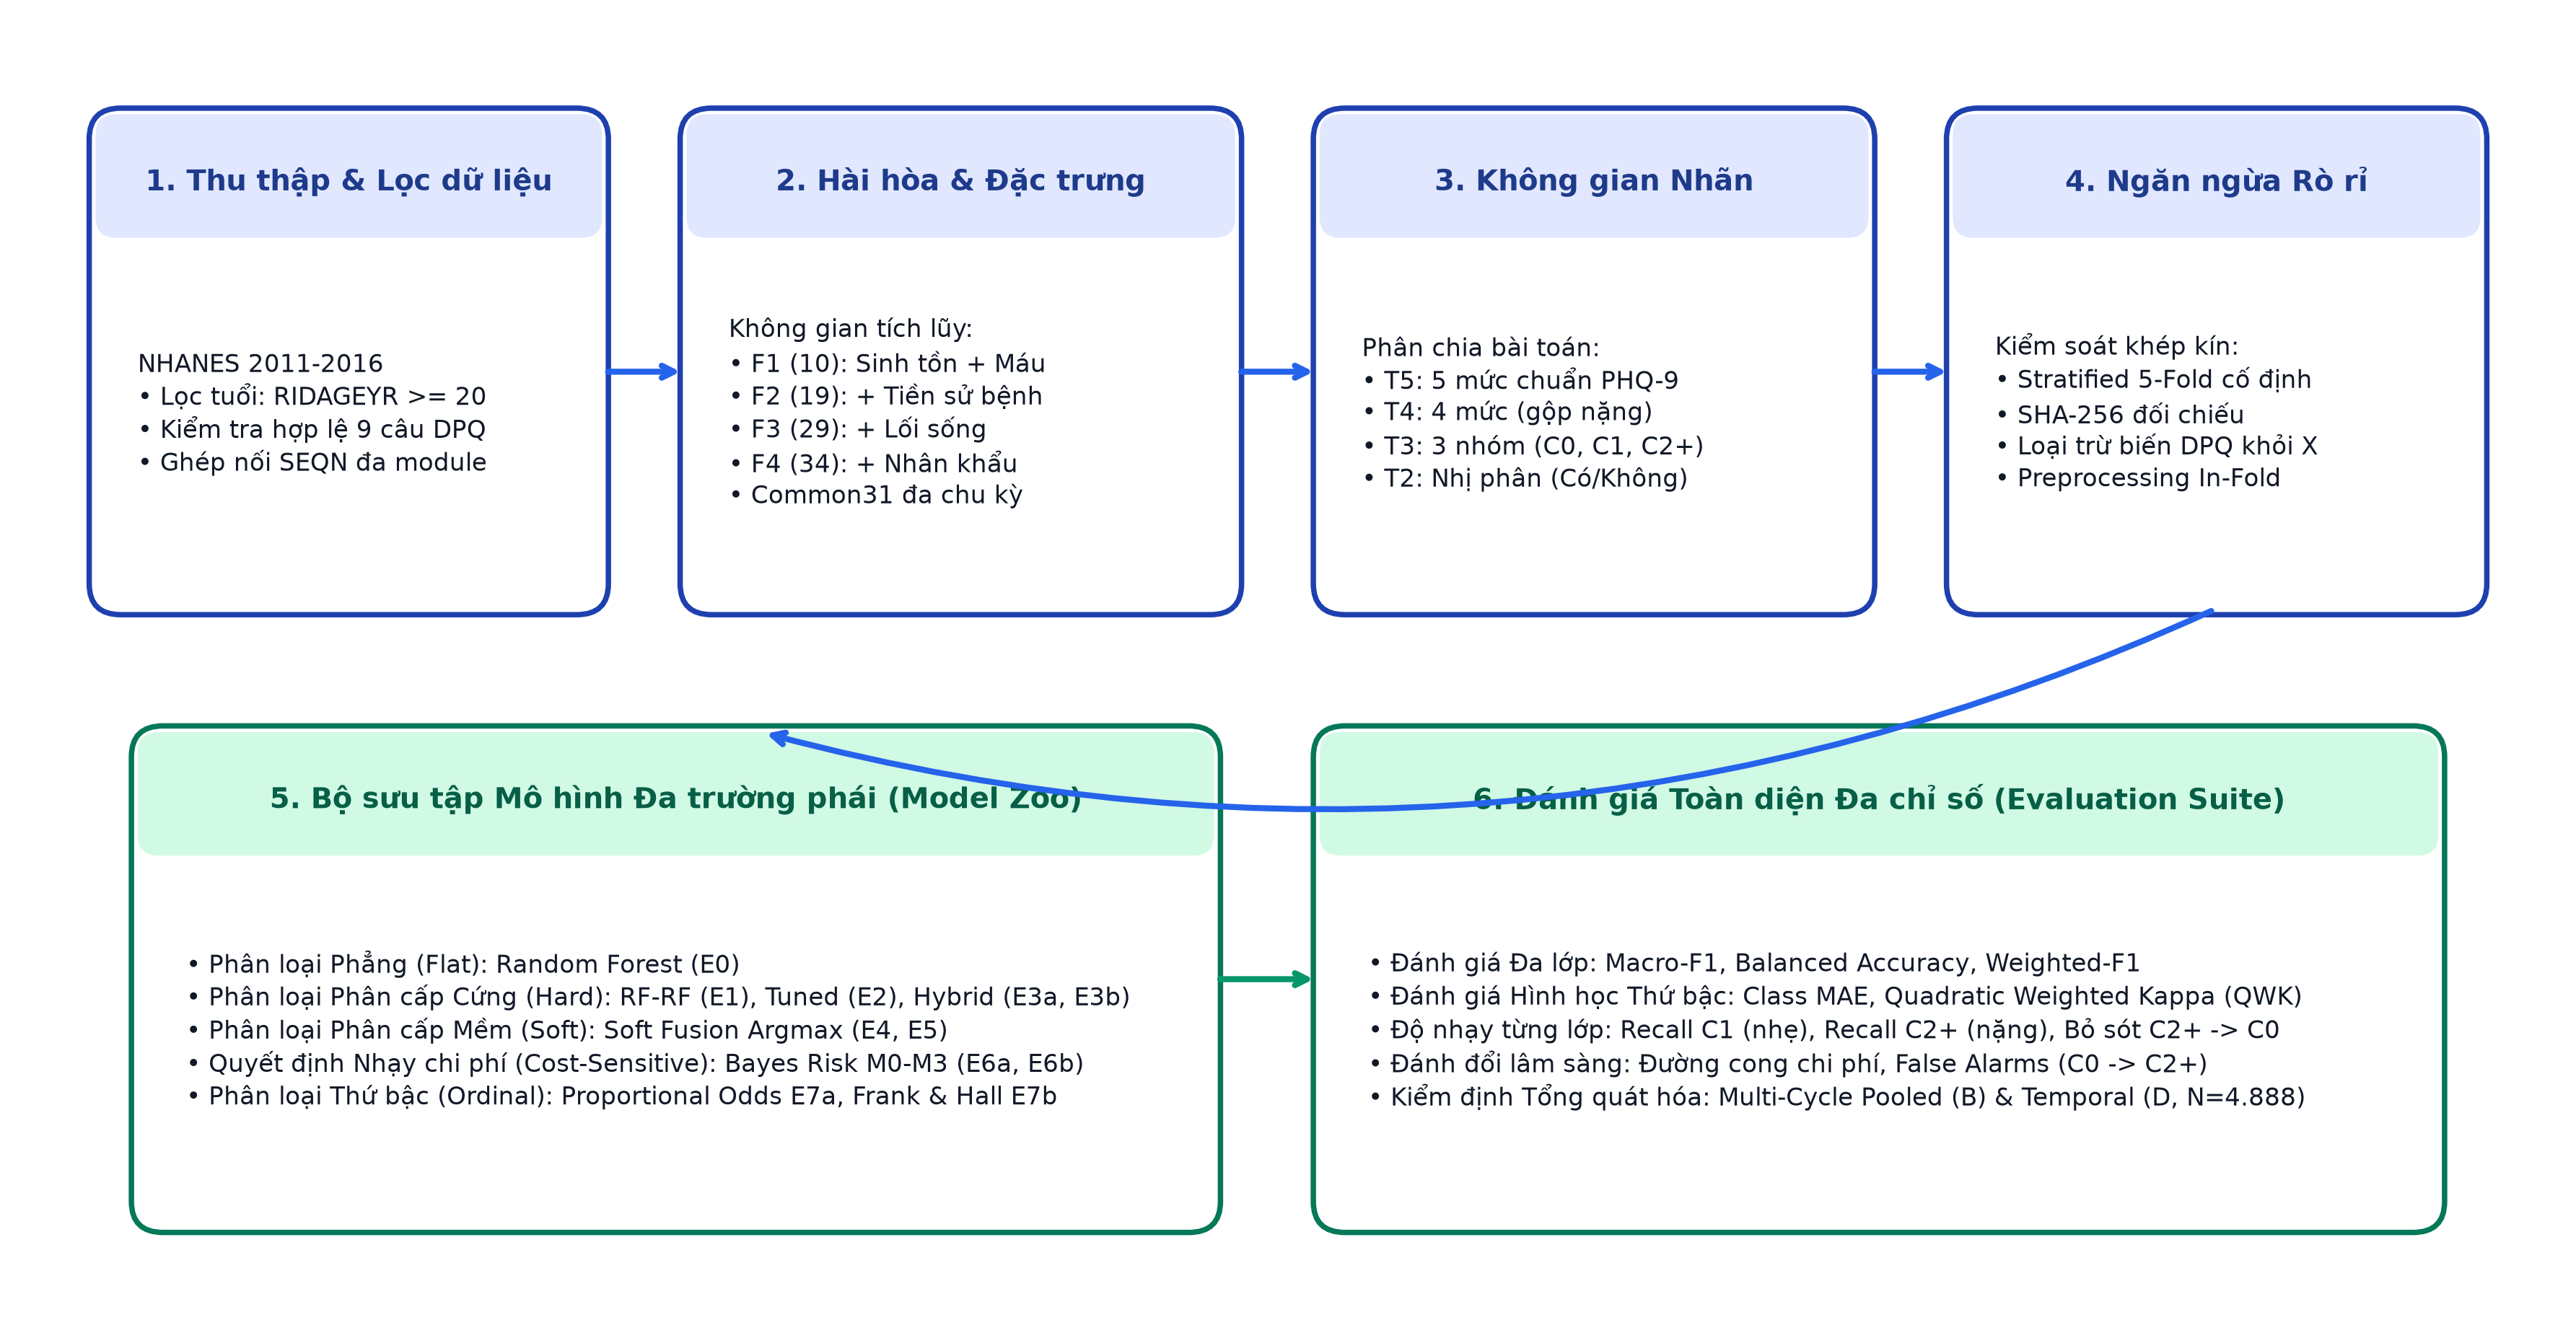
\includegraphics[width=\textwidth]{figures/depsev_overall_architecture.png}
\label{fig:overall-architecture}
\end{figure}
\FloatBarrier

Các cấu phần trong kiến trúc bao gồm:
\begin{enumerate}
    \item \textbf{Data Ingestion \& Filtering:} Tiếp nhận các bảng dữ liệu gốc định dạng SAS Transport (.XPT) hoặc CSV từ NHANES, thực hiện lọc điều kiện người trưởng thành ($\text{RIDAGEYR} \ge 20$) và kiểm tra tính hợp lệ của 9 câu hỏi khảo sát DPQ.
    \item \textbf{Data Harmonization \& Feature Engineering:} Trích xuất các nhóm chỉ số sinh lý, lâm sàng, thói quen sinh hoạt và nhân khẩu học; xử lý chuyển đổi mã hóa các câu hỏi điều hướng phức tạp (như tình trạng hút thuốc và sử dụng rượu bia).
    \item \textbf{Target Construction Module:} Ánh xạ tổng điểm PHQ-9 thành 4 không gian mục tiêu rời rạc ($T_2, T_3, T_4, T_5$).
    \item \textbf{Partitioning \& Isolation Engine:} Quản lý các phân hoạch dữ liệu cố định (Fixed CV Folds, Development/Held-out splits) thông qua mã băm mật mã SHA-256 để bảo đảm khả năng tái lập và ngăn ngừa rò rỉ dữ liệu.
    \item \textbf{Strict In-fold Preprocessing Pipeline:} Thực hiện điền khuyết (median/constant imputation), chuẩn hóa độ lệch chuẩn (StandardScaler) và mã hóa one-hot (OneHotEncoder) nghiêm ngặt bên trong từng training fold.
    \item \textbf{Multi-Paradigm Model Zoo:} Cung cấp các kiến trúc mô hình học máy: Phân loại phẳng (Flat), Phân loại phân cấp (Hard/Soft Hierarchical, Cost-Sensitive Decision) và Phân loại thứ bậc (Ordinal Logistic Regression, Cumulative Binary).
    \item \textbf{Multi-Dimensional Evaluation Suite:} Đánh giá toàn diện trên cả các chỉ số phân loại danh nghĩa (Macro-F1, Balanced Accuracy, Precision/Recall per class) và các chỉ số hình học thứ bậc (Class MAE, Quadratic Weighted Kappa, tỷ lệ lỗi 1 mức và 2 mức).
\end{enumerate}

\section{Dữ liệu nghiên cứu và Hài hòa hóa đa chu kỳ}
\label{sec:du-lieu-nghien-cuu}

Nghiên cứu sử dụng hai tập dữ liệu chính phản ánh hai giai đoạn phát triển của framework:

\subsection{Legacy Development Cohort (NHANES 2013--2014)}
Tập dữ liệu Legacy được xây dựng từ chu kỳ NHANES 2013--2014 kết hợp với tập dữ liệu tiền xử lý chuẩn CDC trên nền tảng Kaggle, có tổng số $N = 5.054$ người tham gia khảo sát đáp ứng điều kiện từ 20 tuổi trở lên và có đầy đủ 9 câu hỏi DPQ:
\begin{itemize}
    \item \textbf{Tập phát triển (Development Partition):} Gồm $N = 4.045$ đối tượng, được sử dụng xuyên suốt cho các thực nghiệm kiểm định chéo Stratified 5-Fold CV, Feature Ablation, Nested CV Tuning, Ensemble và toàn bộ chuỗi thực nghiệm $E_0$--$E_7$.
    \item \textbf{Tập kiểm tra bổ sung (Supplementary Held-out Partition):} Gồm $N = 1.009$ đối tượng được giữ riêng biệt để kiểm tra tham khảo. Cần lưu ý về mặt lai lịch dữ liệu (data provenance): trong quá trình tái cấu trúc phân hoạch chuẩn (split restoration), 813 trong số 1.009 quan sát của tập Held-out từng thuộc tập dữ liệu phát triển ở các phiên bản tiền nghiệm (\texttt{historically\_untouched=false} trong tài liệu kho mã nguồn). Do đó, tập kiểm tra bổ sung này được sử dụng với tính chất đối chứng tham khảo, trong khi toàn bộ các khẳng định hiệu năng khoa học cốt lõi của đề tài được kiểm chứng vững chắc trên quy trình kiểm định chéo Stratified 5-Fold lồng nhau trên tập phát triển ($N = 4.045$).
\end{itemize}

Phân bố nhãn lâm sàng PHQ-9 trên Legacy Cohort được trình bày trong Bảng \ref{tab:legacy-class-dist}.

\begin{table}{Phân bố các lớp triệu chứng PHQ-9 trên Legacy Cohort ($N = 5.054$)}
\centering
\label{tab:legacy-class-dist}
\begin{tabular}{l c c c c c c}
\toprule
\textbf{Phân hoạch} & \textbf{Tổng $N$} & \textbf{$C_0$ (0--4)} & \textbf{$C_1$ (5--9)} & \textbf{$C_2$ (10--14)} & \textbf{$C_3$ (15--19)} & \textbf{$C_4$ (20--27)} \\
\midrule
Development & 4.045 & 3.016 (74.56\%) & 638 (15.77\%) & 243 (6.01\%) & 104 (2.57\%) & 44 (1.09\%) \\
Held-out & 1.009 & 748 (74.13\%) & 162 (16.06\%) & 60 (5.95\%) & 28 (2.78\%) & 11 (1.09\%) \\
\midrule
\textbf{Toàn bộ} & \textbf{5.054} & \textbf{3.764 (74.48\%)} & \textbf{800 (15.83\%)} & \textbf{303 (6.00\%)} & \textbf{132 (2.61\%)} & \textbf{55 (1.09\%)} \\
\bottomrule
\end{tabular}
\end{table}

\subsection{Official Multi-Cycle Cohort (NHANES 2011--2016)}
Để kiểm tra tính tổng quát hóa của các mô hình trên quy mô lớn, nghiên cứu thực hiện quy trình trích xuất và hài hòa hóa dữ liệu (Data Harmonization) từ các bảng dữ liệu gốc chính thức của CDC qua 3 chu kỳ liên tiếp: 2011--2012, 2013--2014 và 2015--2016.

\textbf{Quy trình Hài hòa hóa (Harmonization Protocol):}
Do các chu kỳ NHANES có thể thay đổi thiết kế bảng hỏi hoặc mã định danh biến số phòng xét nghiệm, nghiên cứu đã thực hiện kiểm định schema nghiêm ngặt:
\begin{enumerate}
    \item Ghép nối các bảng module thành phần (Nhân trắc học BMX, Huyết áp BPX, Hóa sinh máu BIOPRO, Huyết học CBC, Cholesterol TCHOL, HDL, HbA1c GHB, Bảng hỏi y tế MCQ, Hút thuốc SMQ, Rượu bia ALQ, Thể lực PAQ, Giấc ngủ SLQ, Nhân khẩu học DEMO và Trầm cảm DPQ) thông qua mã định danh duy nhất SEQN của từng người tham gia.
    \item Loại bỏ các đặc trưng không tương thích: Ví dụ biến số xét nghiệm Triglyceride chỉ được đo trên một phân nhóm mẫu nhịn ăn (fasting sub-sample) ở một số chu kỳ nhất định, gây ra hiện tượng khuyết thiếu cấu trúc (structural missingness) lên tới 50\%; biến này bắt buộc phải loại bỏ để bảo đảm tính nhất quán.
    \item Hợp nhất thành công tập đặc trưng chuẩn $F_{4\_\text{common31}}$ gồm đúng \textbf{31 biến số đồng nhất} trên toàn bộ 3 chu kỳ.
\end{enumerate}

Bảng \ref{tab:multicycle-class-dist} trình bày quy mô và phân bố lớp của các chu kỳ chính thức.

\begin{table}{Phân bố các lớp triệu chứng trên các tập dữ liệu Multi-cycle chính thức}
\centering
\label{tab:multicycle-class-dist}
\begin{tabular}{l c c c c c c}
\toprule
\textbf{Chu kỳ / Phân nhánh} & \textbf{Tổng $N$} & \textbf{$C_0$ (\%)} & \textbf{$C_1$ (\%)} & \textbf{$C_2$ (\%)} & \textbf{$C_3$ (\%)} & \textbf{$C_4$ (\%)} \\
\midrule
NHANES 2011--2012 & 4.639 & 76.12\% & 14.79\% & 5.22\% & 2.61\% & 1.27\% \\
NHANES 2013--2014 (Branch A) & 5.054 & 74.48\% & 15.83\% & 6.00\% & 2.61\% & 1.09\% \\
NHANES 2015--2016 (Branch D Test) & 4.888 & 74.65\% & 17.21\% & 5.03\% & 2.03\% & 1.08\% \\
\midrule
\textbf{Pooled 2011--2016 (Branch B)} & \textbf{14.581} & \textbf{75.06\%} & \textbf{15.96\%} & \textbf{5.42\%} & \textbf{2.41\%} & \textbf{1.15\%} \\
\bottomrule
\end{tabular}
\end{table}

\section{Hệ thống đặc trưng (Feature Spaces)}
\label{sec:he-thong-dac-trung}

Framework DepSev-ML tổ chức 34 biến đầu vào thành 4 nhóm đặc trưng lũy tiến ($F_1 \to F_4$) nhằm phục vụ thực nghiệm cắt bỏ đặc trưng (Feature Ablation Study) theo đúng giao thức chuẩn (\texttt{results/tables/ablation\_feature\_inventory\_final\_protocol.csv}):
\begin{itemize}
    \item \textbf{Nhóm 1 ($F_1$ -- Thể chất, Dấu hiệu sinh tồn \& Xét nghiệm máu, 10 biến):} Gồm 5 chỉ số thể chất và sinh tồn ngoại vi: chỉ số khối cơ thể (BMXBMI), chu vi vòng eo (BMXWAIST), tần số mạch đập khi nghỉ (BPXPLS), trung bình 3 lần đo huyết áp tâm thu (SBP\_mean) và huyết áp tâm trương (DBP\_mean); kết hợp cùng 5 chỉ số xét nghiệm cận lâm sàng máu thiết yếu: Glycohemoglobin HbA1c (LBXGH), Cholesterol toàn phần (LBXTC), HDL-Cholesterol (LBDHDD), Creatinine huyết thanh (LBXSCR) và Albumin huyết thanh (LBXSAL).
    \item \textbf{Nhóm 2 ($F_2$ -- $F_1$ kết hợp Tiền sử bệnh lý lâm sàng, 19 biến):} Bổ sung 9 biến tiền sử bệnh lý và chẩn đoán của bác sĩ: tiền sử tăng huyết áp (BPQ020), đái tháo đường (DIQ010), 5 bệnh lý tim mạch và đột quỵ (MCQ160B, MCQ160C, MCQ160D, MCQ160E, MCQ160F), tiền sử ung thư (MCQ220) và tự đánh giá sức khỏe tổng quát (HUQ010).
    \item \textbf{Nhóm 3 ($F_3$ -- $F_2$ kết hợp Hành vi lối sống \& Giấc ngủ, 29 biến):} Bổ sung 10 chỉ số hành vi sinh hoạt: hoạt động thể lực cường độ mạnh/vừa tại nơi làm việc và giải trí (PAQ605, PAQ620, PAQ650, PAQ665), thời gian ngồi tĩnh tại mỗi ngày (PAD680), tình trạng hút thuốc lá (smoking\_status), thói quen uống rượu bia (ALQ101, alcohol\_status, alcohol\_quantity\_code) và thời lượng giấc ngủ ban đêm (SLD010H).
    \item \textbf{Nhóm 4 ($F_4$ -- Toàn diện kết hợp Nhân khẩu học \& Kinh tế xã hội, 34 biến):} Bổ sung 5 đặc trưng nhân khẩu học quan trọng: Tuổi (RIDAGEYR), Giới tính sinh học (RIAGENDR), Chủng tộc/Dân tộc (RIDRETH1), Trình độ học vấn (DMDEDUC2) và Tỷ lệ thu nhập trên chuẩn nghèo gia đình (INDFMPIR).
\end{itemize}

Trong tập dữ liệu đa chu kỳ $F_{4\_\text{common31}}$, ba biến số không đồng nhất giữa các chu kỳ bị loại bỏ, giữ lại 31 biến số cốt lõi hoàn toàn tương thích. Danh mục chi tiết các biến số được quy định trong Bảng \ref{tab:feature-inventory}.

\begin{longtable}{p{2.5cm} p{2.2cm} p{2.5cm} p{6.5cm}}
\caption{Danh mục hệ thống 34 đặc trưng trong không gian $F_4$ theo giao thức chính thức} \label{tab:feature-inventory} \\
\toprule
\textbf{Mã biến} & \textbf{Nhóm đặc trưng} & \textbf{Kiểu dữ liệu} & \textbf{Mô tả lâm sàng / ý nghĩa} \\
\midrule
\endfirsthead
\toprule
\textbf{Mã biến} & \textbf{Nhóm đặc trưng} & \textbf{Kiểu dữ liệu} & \textbf{Mô tả lâm sàng / ý nghĩa} \\
\midrule
\endhead
\bottomrule
\endfoot
\multicolumn{4}{l}{\textbf{Nhóm $F_1$ (10 đặc trưng): Dấu hiệu sinh tồn, Nhân trắc \& Xét nghiệm máu}} \\
BMXBMI & Thể chất ($F_1$) & Liên tục (kg/m$^2$) & Chỉ số khối cơ thể (Body Mass Index) \\
BMXWAIST & Thể chất ($F_1$) & Liên tục (cm) & Chu vi vòng eo (đo lường béo phì trung tâm) \\
BPXPLS & Sinh tồn ($F_1$) & Rời rạc (nhịp/phút) & Tần số mạch đập khi nghỉ ngơi (60 giây) \\
SBP\_mean & Sinh tồn ($F_1$) & Liên tục (mmHg) & Huyết áp tâm thu trung bình qua các lần đo \\
DBP\_mean & Sinh tồn ($F_1$) & Liên tục (mmHg) & Huyết áp tâm trương trung bình qua các lần đo \\
LBXGH & Cận lâm sàng ($F_1$) & Liên tục (\%) & Glycohemoglobin (HbA1c - chuyển hóa đường) \\
LBXTC & Cận lâm sàng ($F_1$) & Liên tục (mg/dL) & Cholesterol toàn phần huyết thanh \\
LBDHDD & Cận lâm sàng ($F_1$) & Liên tục (mg/dL) & HDL-Cholesterol (cholesterol tỷ trọng cao) \\
LBXSCR & Cận lâm sàng ($F_1$) & Liên tục (mg/dL) & Creatinine huyết thanh (chức năng lọc của thận) \\
LBXSAL & Cận lâm sàng ($F_1$) & Liên tục (g/dL) & Albumin huyết thanh (chức năng gan, dinh dưỡng) \\
\midrule
\multicolumn{4}{l}{\textbf{Nhóm $F_2$ (19 đặc trưng): $F_1$ + 9 tiền sử bệnh lý lâm sàng}} \\
BPQ020 & Tiền sử ($F_2$) & Phân loại nhị phân & Bác sĩ từng chẩn đoán Tăng huyết áp \\
DIQ010 & Tiền sử ($F_2$) & Phân loại nhị phân & Bác sĩ từng chẩn đoán Đái tháo đường \\
MCQ160B & Tiền sử ($F_2$) & Phân loại nhị phân & Bác sĩ từng chẩn đoán Suy tim sung huyết \\
MCQ160C & Tiền sử ($F_2$) & Phân loại nhị phân & Bác sĩ từng chẩn đoán Bệnh tim mạch vành \\
MCQ160D & Tiền sử ($F_2$) & Phân loại nhị phân & Bác sĩ từng chẩn đoán Đau thắt ngực \\
MCQ160E & Tiền sử ($F_2$) & Phân loại nhị phân & Tiền sử từng bị Cơn đau tim / Nhồi máu cơ tim \\
MCQ160F & Tiền sử ($F_2$) & Phân loại nhị phân & Tiền sử từng bị Đột quỵ / Tai biến mạch máu não \\
MCQ220 & Tiền sử ($F_2$) & Phân loại nhị phân & Tiền sử từng được chẩn đoán mắc Ung thư \\
HUQ010 & Lâm sàng ($F_2$) & Thứ bậc (1--5) & Tự đánh giá tình trạng sức khỏe tổng quát \\
\midrule
\multicolumn{4}{l}{\textbf{Nhóm $F_3$ (29 đặc trưng): $F_2$ + 10 hành vi lối sống \& giấc ngủ}} \\
PAQ605, PAQ620 & Lối sống ($F_3$) & Phân loại nhị phân & Hoạt động thể lực cường độ mạnh / vừa tại nơi làm việc \\
PAQ650, PAQ665 & Lối sống ($F_3$) & Phân loại nhị phân & Hoạt động thể lực cường độ mạnh / vừa trong giải trí \\
PAD680 & Lối sống ($F_3$) & Liên tục (phút/ngày) & Thời gian ngồi tĩnh tại trung bình mỗi ngày \\
smoking\_status & Lối sống ($F_3$) & Phân loại 3 mức & Tình trạng hút thuốc lá (Never, Former, Current) \\
ALQ101 & Lối sống ($F_3$) & Phân loại nhị phân & Uống ít nhất 12 đồ uống có cồn trong năm qua \\
alcohol\_status & Lối sống ($F_3$) & Phân loại 3 mức & Tình trạng dùng rượu bia (Non, Moderate, Heavy) \\
alcohol\_qty & Lối sống ($F_3$) & Thứ bậc lượng hóa & Mức độ tiêu thụ rượu bia lượng hóa \\
SLD010H & Lối sống ($F_3$) & Liên tục (giờ) & Thời lượng giấc ngủ thông thường mỗi đêm \\
\midrule
\multicolumn{4}{l}{\textbf{Nhóm $F_4$ (34 đặc trưng): $F_3$ + 5 nhân khẩu học \& kinh tế xã hội}} \\
RIDAGEYR & Nhân khẩu ($F_4$) & Liên tục (tuổi) & Tuổi của người tham gia khảo sát tại thời điểm khám \\
RIAGENDR & Nhân khẩu ($F_4$) & Phân loại nhị phân & Giới tính sinh học (Nam / Nữ) \\
RIDRETH1 & Nhân khẩu ($F_4$) & Phân loại 5 nhóm & Chủng tộc / Dân tộc tự xác định \\
DMDEDUC2 & Nhân khẩu ($F_4$) & Thứ bậc (1--5) & Trình độ học vấn cao nhất đạt được (người lớn) \\
INDFMPIR & Kinh tế ($F_4$) & Liên tục (tỷ số) & Tỷ số thu nhập gia đình trên chuẩn nghèo liên bang \\
\end{longtable}


\section{Tiền xử lý dữ liệu và Quy trình chống rò rỉ (Leakage Controls)}
\label{sec:tien-xu-ly}

Dữ liệu y tế luôn đối mặt với vấn đề giá trị khuyết thiếu (missing data) và sự không đồng nhất về thang đo. Một trong những sai lầm phổ biến nhất trong các nghiên cứu học máy y tế là áp dụng các phép biến đổi dữ liệu (chuẩn hóa, điền khuyết) trên toàn bộ tập dữ liệu trước khi chia fold, dẫn đến việc phân phối của tập kiểm tra bị rò rỉ vào tập huấn luyện (Data Leakage).

Trong DepSev-ML, quy trình tiền xử lý được đóng gói trong một \texttt{scikit-learn Pipeline} hoàn toàn cô lập:
\begin{enumerate}
    \item \textbf{Xử lý biến số liên tục (Numerical Pipeline):}
    \begin{itemize}
        \item Điền khuyết bằng trung vị (Median Imputation): Giá trị trung vị $\tilde{x}_j$ được tính toán \textbf{duy nhất trên tập huấn luyện của fold hiện tại} và được áp dụng để điền các ô trống trên cả tập huấn luyện và tập kiểm tra.
        \item Chuẩn hóa Z-score (Standard Scaling): Biến đổi $z = (x - \mu) / \sigma$ trong đó giá trị trung bình $\mu$ và độ lệch chuẩn $\sigma$ được học hoàn toàn từ tập huấn luyện.
    \end{itemize}
    \item \textbf{Xử lý biến số phân loại (Categorical Pipeline):}
    \begin{itemize}
        \item Điền khuyết bằng hằng số: Các ô khuyết thiếu hoặc không xác định được gán nhãn chuỗi cố định \texttt{"missing\_or\_unknown"}.
        \item Mã hóa One-Hot (OneHotEncoder): Thiết lập tham số \texttt{handle\_unknown='ignore'} và \texttt{sparse\_output=False}. Nếu trên tập kiểm tra xuất hiện một danh mục chưa từng gặp trong tập huấn luyện, vectơ mã hóa one-hot tương ứng sẽ tự động gán toàn bộ bằng 0 mà không gây lỗi thực thi.
    \end{itemize}
    \item \textbf{Loại trừ tuyệt đối các biến mục tiêu DPQ:} Không có bất kỳ câu hỏi nào trong số 9 câu hỏi DPQ hay tổng điểm PHQ-9 được phép xuất hiện trong ma trận đặc trưng $\mathbf{X}$.
\end{enumerate}

Sơ đồ thực thi tiền xử lý bên trong kiểm định chéo được mô tả trong Thuật toán \ref{algo:cv-leakage-free}.

\begin{algorithm}[h!]
\SetAlgoLined
\KwIn{Tập dữ liệu $\mathcal{D} = \{(\mathbf{x}_i, y_i)\}_{i=1}^N$, số lượng folds $K=5$, kiến trúc mô hình $\mathcal{M}$}
\KwOut{Tập hợp dự đoán out-of-fold $\hat{\mathbf{y}}_{\text{oof}}$, các độ đo hiệu năng trung bình}
Khởi tạo phân hoạch Stratified 5-Fold: $\{\mathcal{S}_1, \dots, \mathcal{S}_5\} \leftarrow \text{StratifiedKFold}(\mathcal{D}, K=5, \text{seed}=42)$\;
Khởi tạo mảng dự đoán $\hat{\mathbf{y}}_{\text{oof}} \leftarrow \text{zeros}(N)$\;
\For{$k = 1$ \KwTo $5$}{
    $\mathcal{D}_{\text{val}} \leftarrow \mathcal{S}_k$; \quad $\mathcal{D}_{\text{train}} \leftarrow \mathcal{D} \setminus \mathcal{S}_k$\;
    Khởi tạo Pipeline tiền xử lý $\mathcal{P}_k$\;
    $\mathcal{P}_k.\text{fit}(\mathbf{X}_{\text{train}})$ \tcp*{Chỉ fit trên tập train!}
    $\mathbf{X}_{\text{train\_trans}} \leftarrow \mathcal{P}_k.\text{transform}(\mathbf{X}_{\text{train}})$\;
    $\mathbf{X}_{\text{val\_trans}} \leftarrow \mathcal{P}_k.\text{transform}(\mathbf{X}_{\text{val}})$ \tcp*{Transform tập val bằng tham số của train}
    Huấn luyện mô hình: $\mathcal{M}_k.\text{fit}(\mathbf{X}_{\text{train\_trans}}, \mathbf{y}_{\text{train}})$\;
    Dự đoán trên tập kiểm tra: $\hat{\mathbf{y}}_{\text{val}} \leftarrow \mathcal{M}_k.\text{predict}(\mathbf{X}_{\text{val\_trans}})$\;
    Lưu dự đoán: $\hat{\mathbf{y}}_{\text{oof}}[\mathcal{S}_k] \leftarrow \hat{\mathbf{y}}_{\text{val}}$\;
    Tính toán các chỉ số fold $k$: $\text{Macro-F1}_k, \text{BalAcc}_k, \text{MAE}_k$\;
}
Tính trung bình và độ lệch chuẩn của các chỉ số qua 5 folds\;
\Return{$\hat{\mathbf{y}}_{\text{oof}}$, Bảng tổng hợp hiệu năng}\;
\caption{Quy trình kiểm định chéo Stratified 5-Fold không rò rỉ dữ liệu trong DepSev-ML}
\label{algo:cv-leakage-free}
\end{algorithm}

\subsection{Lưu ý về Thiết kế mẫu khảo sát phức hợp (Complex Survey Design)}
\label{subsec:nhanes-survey-design-note}
Khảo sát NHANES áp dụng thiết kế chọn mẫu xác suất phân tầng, phân cụm nhiều giai đoạn (multistage, stratified, clustered probability sampling) đại diện cho toàn bộ dân số không nằm trong viện của Hoa Kỳ, đi kèm trọng số lấy mẫu (\texttt{WTINT2YR}, \texttt{WTMEC2YR}) và các biến số phân tầng (\texttt{SDMVSTRA}, \texttt{SDMVPSU}). 

Trong khuôn khổ nghiên cứu học máy thực nghiệm tiêu chuẩn của đề tài, các mô hình được tối ưu hóa theo nguyên lý tối thiểu hóa rủi ro thực nghiệm không trọng số (Unweighted Empirical Risk Minimization -- ERM) trên tập mẫu có sẵn, phù hợp với các tiêu chuẩn benchmark học máy y tế hiện hành. Tuy nhiên, về mặt dịch tễ học và suy luận thống kê quần thể chính thống, các ước lượng này không phản ánh hoàn toàn xác suất đại diện dịch tễ trên toàn dân số Hoa Kỳ. Nghiên cứu ghi nhận đây là một giới hạn phương pháp luận quan trọng cần được mở rộng trong tương lai thông qua việc tích hợp hàm hợp lý giả có trọng số (Survey-weighted Pseudo-likelihood).

\section{Thiết kế các mô hình Phân loại phân cấp và Nhạy chi phí}
\label{sec:thiet-ke-hierarchical}

\subsection{Hard Hierarchical Classification ($E_1, E_2, E_3a, E_3b$)}
Hệ thống phân cấp hai tầng cứng hoạt động theo cơ chế tuần tự:
\begin{itemize}
    \item \textbf{Bộ phân loại Tầng 1 ($M_{\text{Stage1}}$):} Được huấn luyện trên toàn bộ tập huấn luyện với nhãn $z_1 = \mathbb{I}(s \ge 5)$. Mục tiêu là phát hiện người có bất kỳ triệu chứng trầm cảm nào.
    \item \textbf{Bộ phân loại Tầng 2 ($M_{\text{Stage2}}$):} Chỉ được huấn luyện trên phân nhóm mẫu có triệu chứng ($s \ge 5$), phân biệt giữa $C_1$ ($s \in [5, 9]$, gán nhãn 0) và $C_2^+$ ($s \in [10, 27]$, gán nhãn 1).
\end{itemize}

Dự đoán được thực hiện theo quy tắc:
\begin{equation}
    \hat{y} = \begin{cases} 0 & \text{nếu } P(Y \ge 1 \mid \mathbf{x}) < \tau_1 \\ 1 & \text{nếu } P(Y \ge 1 \mid \mathbf{x}) \ge \tau_1 \land P(Y = 2 \mid Y \ge 1, \mathbf{x}) < \tau_2 \\ 2 & \text{nếu } P(Y \ge 1 \mid \mathbf{x}) \ge \tau_1 \land P(Y = 2 \mid Y \ge 1, \mathbf{x}) \ge \tau_2 \end{cases}
\end{equation}
Trong mô hình $E_1$, ngưỡng cắt mặc định $\tau_1 = \tau_2 = 0.5$. Trong mô hình $E_2$, hai ngưỡng được tối ưu hóa đồng thời trên không gian lưới thông qua kiểm định chéo nội bộ.

\subsection{Soft Hierarchical kết hợp Tối ưu rủi ro Bayes ($E_4, E_5, E_6a, E_6b$)}
Khắc phục nhược điểm của Hard Routing, mô hình Soft Hierarchical suy diễn phân phối xác suất hợp thành trên toàn bộ không gian 3 lớp thông qua các công thức (\ref{eq:soft-p0})--(\ref{eq:soft-p2}).

Sau khi thu được vectơ xác suất $\mathbf{p}(\mathbf{x}) = [P(C_0), P(C_1), P(C_2^+)]$, quyết định được đưa ra bằng cách tối thiểu hóa rủi ro kỳ vọng theo ma trận chi phí $\mathbf{K}$:
\begin{equation}
    \hat{y} = \arg\min_{j \in \{0, 1, 2\}} \sum_{i=0}^2 P(C_i \mid \mathbf{x}) \cdot K_{ij}
\end{equation}

Bốn ứng viên ma trận chi phí được thiết kế:
\begin{itemize}
    \item \textbf{$M_0$ (Mất mát đồng nhất 0--1, tương đương Argmax):}
    \begin{equation}
        \mathbf{K}_{M0} = \begin{bmatrix} 0 & 1 & 1 \\ 1 & 0 & 1 \\ 1 & 1 & 0 \end{bmatrix}
    \end{equation}
    \item \textbf{$M_1$ (Phạt vừa ca bỏ sót nặng):}
    \begin{equation}
        \mathbf{K}_{M1} = \begin{bmatrix} 0.0 & 1.0 & 1.5 \\ 1.5 & 0.0 & 1.0 \\ 3.0 & 1.5 & 0.0 \end{bmatrix}
    \end{equation}
    \item \textbf{$M_2$ (Phạt nặng ca bỏ sót):}
    \begin{equation}
        \mathbf{K}_{M2} = \begin{bmatrix} 0.0 & 1.0 & 2.0 \\ 2.0 & 0.0 & 1.0 \\ 5.0 & 2.0 & 0.0 \end{bmatrix}
    \end{equation}
    \item \textbf{$M_3$ (Phạt cực đoan ca bỏ sót):}
    \begin{equation}
        \mathbf{K}_{M3} = \begin{bmatrix} 0.0 & 1.0 & 2.5 \\ 2.5 & 0.0 & 1.0 \\ 8.0 & 3.0 & 0.0 \end{bmatrix}
    \end{equation}
\end{itemize}

Thuật toán \ref{algo:soft-cost-sensitive} mô tả chi tiết quy trình dự đoán của mô hình Soft Cost-Sensitive.

\begin{algorithm}[h!]
\SetAlgoLined
\KwIn{Mẫu kiểm tra $\mathbf{x}$, bộ phân loại Tầng 1 $M_{\text{Stage1}}$, bộ phân loại Tầng 2 $M_{\text{Stage2}}$, ma trận chi phí $\mathbf{K}$}
\KwOut{Nhãn dự đoán $\hat{y} \in \{0, 1, 2\}$}
Tính xác suất có triệu chứng: $p_1 \leftarrow M_{\text{Stage1}}.\text{predict\_proba}(\mathbf{x})[:, 1]$\;
Tính xác suất nặng có điều kiện: $p_2 \leftarrow M_{\text{Stage2}}.\text{predict\_proba}(\mathbf{x})[:, 1]$\;
Tích hợp phân phối xác suất 3 lớp:\\
$P(C_0) \leftarrow 1.0 - p_1$\;
$P(C_1) \leftarrow p_1 \cdot (1.0 - p_2)$\;
$P(C_2^+) \leftarrow p_1 \cdot p_2$\;
$\mathbf{P} \leftarrow [P(C_0), P(C_1), P(C_2^+)]$\;
Chuẩn hóa bảo đảm $\sum P(C_k) = 1.0$ và $P(C_k) \ge 0$\;
Tính ma trận rủi ro kỳ vọng: $\mathbf{R} \leftarrow \mathbf{P} \times \mathbf{K}$\;
Chọn nhãn có rủi ro nhỏ nhất: $\hat{y} \leftarrow \arg\min_j R_j$\;
\Return{$\hat{y}$}\;
\caption{Quy trình suy diễn xác suất mềm và quyết định nhạy chi phí ($E_6$)}
\label{algo:soft-cost-sensitive}
\end{algorithm}

\section{Thiết kế các mô hình Phân loại thứ bậc ($E_7$)}
\label{sec:thiet-ke-ordinal}

\subsection{E7a – Ordinal Logistic Regression (Proportional Odds)}
Để bảo đảm tính ổn định và tính tự chủ công nghệ tuyệt đối trên Python 3.13, mô hình \texttt{OrdinalLogisticRegression} được hiện thực trực tiếp từ nguyên lý biến tiềm ẩn. 

\textbf{Tái tham số hóa khử ràng buộc bảo đảm tính đơn điệu:}
Hai ngưỡng cắt $\theta_0$ và $\theta_1$ bắt buộc phải thỏa mãn $\theta_0 < \theta_1$. Thay vì giải bài toán tối ưu có ràng buộc phức tạp, nghiên cứu áp dụng kỹ thuật đổi biến số mũ:
\begin{align}
    \theta_0 &= \alpha \\
    \theta_1 &= \alpha + \exp(\delta), \quad \text{với } \alpha \in \mathbb{R}, \delta \in \mathbb{R}
\end{align}
Khi đó, hiệu số $\theta_1 - \theta_0 = \exp(\delta) > 0$ được bảo đảm luôn dương nghiêm ngặt với mọi giá trị của $\delta \in (-\infty, +\infty)$. Không gian tối ưu trở thành không gian tự do $\mathbb{R}^{d+2}$ đối với vectơ tham số $\mathbf{\Theta} = [\mathbf{w}^T, \alpha, \delta]^T$.

\textbf{Hàm mất mát và Gradient giải tích:}
Hàm mất mát Negative Log-Likelihood có trọng số mẫu $s_i$ và điều chuẩn $L_2$ trên vectơ trọng số $\mathbf{w}$ (không phạt các ngưỡng cắt):
\begin{equation}
    \mathcal{L}(\mathbf{w}, \alpha, \delta) = - \sum_{i=1}^N s_i \log P(Y = y_i \mid \mathbf{x}_i) + \frac{1}{2C} \|\mathbf{w}\|^2
\end{equation}

Đặt $z_{0i} = \alpha - \mathbf{w}^T \mathbf{x}_i$ và $z_{1i} = \alpha + e^\delta - \mathbf{w}^T \mathbf{x}_i$. Xác suất tương ứng là $\sigma_{0i} = \sigma(z_{0i})$ và $\sigma_{1i} = \sigma(z_{1i})$. Đạo hàm riêng giải tích theo từng tham số được dẫn xuất chính xác:
\begin{align}
    \frac{\partial \mathcal{L}}{\partial \mathbf{w}} &= - \sum_{i=1}^N s_i (g_{0i} + g_{1i}) \mathbf{x}_i + \frac{1}{C} \mathbf{w} \\
    \frac{\partial \mathcal{L}}{\partial \alpha} &= \sum_{i=1}^N s_i (g_{0i} + g_{1i}) \\
    \frac{\partial \mathcal{L}}{\partial \delta} &= e^\delta \sum_{i=1}^N s_i g_{1i}
\end{align}
trong đó các đại lượng $g_{0i}, g_{1i}$ được tính theo nhãn thực tế $y_i$:
\begin{equation}
    (g_{0i}, g_{1i}) = \begin{cases} (-(1 - \sigma_{0i}), 0) & \text{nếu } y_i = 0 \\ \left(\frac{\sigma_{0i}(1 - \sigma_{0i})}{\sigma_{1i} - \sigma_{0i}}, -\frac{\sigma_{1i}(1 - \sigma_{1i})}{\sigma_{1i} - \sigma_{0i}}\right) & \text{nếu } y_i = 1 \\ (0, \sigma_{1i}) & \text{nếu } y_i = 2 \end{cases}
\end{equation}

Mô hình được tối ưu hóa bằng thuật toán L-BFGS-B với độ chính xác cao.

\subsection{E7b – Cumulative Binary Classification (Frank \& Hall 2001)}
Quy trình huấn luyện và suy diễn của phương pháp Frank \& Hall kết hợp phép chiếu bình phương tối thiểu được mô tả trong Thuật toán \ref{algo:frank-hall}.

\begin{algorithm}[h!]
\SetAlgoLined
\KwIn{Mẫu kiểm tra $\mathbf{x}$, bộ phân loại $M_1$ dự đoán $P(Y \ge 1)$, bộ phân loại $M_2$ dự đoán $P(Y \ge 2)$}
\KwOut{Phân phối xác suất hợp lệ $\mathbf{p} = [P(C_0), P(C_1), P(C_2^+)]$}
Dự đoán xác suất thô: $q_1 \leftarrow M_1.\text{predict\_proba}(\mathbf{x})[:, 1]$; \quad $q_2 \leftarrow M_2.\text{predict\_proba}(\mathbf{x})[:, 1]$\;
\eIf{$q_2 > q_1$ \tcp*{Vi phạm tính đơn điệu!}}{
    Ghi nhận vi phạm đơn điệu (Monotonicity Violation)\;
    Áp dụng phép chiếu bình phương tối thiểu đẳng điệu:\\
    $q_1' \leftarrow \frac{q_1 + q_2}{2}$; \quad $q_2' \leftarrow \frac{q_1 + q_2}{2}$\;
}{
    $q_1' \leftarrow q_1$; \quad $q_2' \leftarrow q_2$\;
}
Tính xác suất từng lớp:\\
$P(C_0) \leftarrow 1.0 - q_1'$\;
$P(C_1) \leftarrow q_1' - q_2'$\;
$P(C_2^+) \leftarrow q_2'$\;
\Return{$[P(C_0), P(C_1), P(C_2^+)]$}\;
\caption{Quy trình suy diễn Frank \& Hall với phép chiếu đẳng điệu ($E_7b$)}
\label{algo:frank-hall}
\end{algorithm}

\section{Hệ thống thước đo đánh giá (Evaluation Metrics)}
\label{sec:he-thong-thuoc-do}

Để đánh giá toàn diện và phản ánh đúng bản chất bài toán mất cân bằng lớp và phân loại có thứ tự, DepSev-ML sử dụng hệ thống độ đo đa chiều:

\subsection{Các chỉ số phân loại danh nghĩa}
\begin{enumerate}
    \item \textbf{Độ chính xác (Accuracy):}
    \begin{equation}
        \text{Accuracy} = \frac{1}{N} \sum_{i=1}^N \mathbb{I}(y_i = \hat{y}_i)
    \end{equation}
    \textit{Lưu ý phương pháp luận:} Trên dữ liệu mất cân bằng ($C_0$ chiếm 75\%), một mô hình tầm thường (trivial majority baseline) dự đoán toàn bộ là $C_0$ vẫn đạt Accuracy = 74.56\%, nhưng hoàn toàn vô giá trị về mặt y tế. Do đó Accuracy không thể được sử dụng làm chỉ số quyết định.
    \item \textbf{Độ chính xác cân bằng (Balanced Accuracy):}
    \begin{equation}
        \text{Balanced Accuracy} = \frac{1}{K} \sum_{k=0}^{K-1} \text{Recall}_k = \frac{1}{K} \sum_{k=0}^{K-1} \frac{\text{TP}_k}{\text{TP}_k + \text{FN}_k}
    \end{equation}
    Độ đo này triệt tiêu hoàn toàn ưu thế kích thước của lớp đa số bằng cách tính trung bình cộng không trọng số của độ nhạy (Recall) trên từng lớp riêng biệt. Đối với mô hình tầm thường dồn lớp, Balanced Accuracy chỉ đạt đúng $1/K$ (33.33\% trên $T_3$ hoặc 20.0\% trên $T_5$).
    \item \textbf{Macro-averaged F1-score (Macro-F1):}
    \begin{equation}
        \text{Macro-F1} = \frac{1}{K} \sum_{k=0}^{K-1} \text{F1}_k = \frac{1}{K} \sum_{k=0}^{K-1} \frac{2 \cdot \text{Precision}_k \cdot \text{Recall}_k}{\text{Precision}_k + \text{Recall}_k}
    \end{equation}
    Đóng vai trò là \textbf{thước đo chất lượng chính (Primary Metric)} của toàn bộ nghiên cứu.
\end{enumerate}

\subsection{Các chỉ số khoảng cách thứ bậc (Ordinal Metrics)}
\begin{enumerate}
    \item \textbf{Sai số tuyệt đối trung bình theo lớp (Class MAE):}
    \begin{equation}
        \text{Class MAE} = \frac{1}{N} \sum_{i=1}^N |y_i - \hat{y}_i|
    \end{equation}
    với $y_i, \hat{y}_i \in \{0, 1, \dots, K-1\}$. Cần phân biệt rõ: Class MAE được tính trên không gian chỉ số lớp nguyên rời rạc, \textbf{không phải sai số MAE trên tổng điểm PHQ-9 liên tục} $s \in [0, 27]$.
    \item \textbf{Hệ số Kappa Cohen trọng số bậc hai (Quadratic Weighted Kappa -- QWK) \cite{cohen1968weighted}:}
    \begin{equation}
        \kappa_w = 1 - \frac{\sum_{i,j} W_{ij} O_{ij}}{\sum_{i,j} W_{ij} E_{ij}}
    \end{equation}
    trong đó $O_{ij}$ là ma trận nhầm lẫn quan sát được, $E_{ij}$ là ma trận kỳ vọng ngẫu nhiên, và ma trận trọng số phạt bậc hai $W_{ij} = \frac{(i - j)^2}{(K - 1)^2}$. QWK phạt các sai lầm cách xa nhau theo bình phương khoảng cách thứ bậc.
    \item \textbf{Tỷ lệ lỗi 1 mức và lỗi 2 mức (1-Step and 2-Step Error Rates):}
    \begin{align}
        \text{Error}_{\text{1-step}} &= \frac{1}{N} \sum_{i=1}^N \mathbb{I}(|y_i - \hat{y}_i| = 1) \\
        \text{Error}_{\text{2-step}} &= \frac{1}{N} \sum_{i=1}^N \mathbb{I}(|y_i - \hat{y}_i| = 2)
    \end{align}
    Trong đó, các ca sai lệch 2 mức bao gồm hai hướng đối lập: $C_2^+ \to C_0$ (Bỏ sót bệnh nhân nặng sang bình thường) và $C_0 \to C_2^+$ (Báo động giả người bình thường thành rất nặng).
\end{enumerate}

\section{Tóm tắt chương và kết nối thực nghiệm}
\label{sec:tom-tat-chuong-3}

Chương \ref{ch:phuong-phap} đã hoàn thiện việc đặc tả toàn bộ phương pháp luận và thiết kế thực nghiệm của khung làm việc DepSev-ML. Nghiên cứu đã thiết lập một chu trình xử lý dữ liệu chuẩn hóa từ hai tập dữ liệu độc lập: Legacy Cohort ($N=5.054$) phục vụ huấn luyện và kiểm định chéo Stratified 5-Fold không rò rỉ, và Harmonized Multi-Cycle Cohort ($N=14.581$) phục vụ đánh giá quy mô lớn và kiểm tra suy giảm hiệu năng theo thời gian (Temporal Evaluation). Hệ thống 31 đặc trưng chung được cấu trúc lũy tiến thành các tập $F_1 \to F_4$, kết hợp cùng quy trình chuẩn hóa và điền khuyết nghiêm ngặt in-fold. Đồng thời, nghiên cứu đã xây dựng một sở thú mô hình đa trường phái bao gồm Flat Classification, Hard Hierarchical ($E_1$--$E_3$), Soft Hierarchical ($E_4$--$E_5$), Cost-Sensitive Decision ($E_6$), và Ordinal Classification ($E_7$), đi kèm hệ thống chỉ số đánh giá đa chiều (Macro-F1, Balanced Accuracy, Class MAE, QWK, và lỗi sai lệch 1--2 mức).

Toàn bộ các quy tắc thực nghiệm, phân hoạch tập dữ liệu và mô hình được đặc tả trong chương này là cơ sở duy nhất để triển khai các phân tích thực nghiệm và đối chiếu số liệu trong Chương \ref{ch:ket-qua-thao-luan}.
\cleardoublepage

\chapter{Thực nghiệm và đánh giá}
\label{ch:thuc-nghiem}

\section{Môi trường thực nghiệm}
\label{sec:moi-truong-thuc-nghiem}

Để đảm bảo tính khả lập (reproducibility) và tính minh bạch tuyệt đối của toàn bộ quá trình nghiên cứu, tất cả các thực nghiệm trong framework DepSev-ML được thực thi trên môi trường phần cứng và phần mềm chuẩn tắc:
\begin{itemize}
    \item \textbf{Phần cứng (Hardware):} Máy trạm cá nhân Apple Silicon (kiến trúc ARM64, vi xử lý Apple M-series), bộ nhớ RAM 16 GB, ổ cứng thể rắn SSD tốc độ cao.
    \item \textbf{Hệ điều hành (Operating System):} macOS (Darwin Kernel Version 24.6.0).
    \item \textbf{Môi trường phần mềm và Ngôn ngữ lập trình:} Python phiên bản 3.13.7 (Clang 16.0.0) chạy trong môi trường ảo hóa độc lập (\texttt{.venv}).
    \item \textbf{Các thư viện tính toán khoa học cốt lõi:}
    \begin{itemize}
        \item \texttt{scikit-learn}: Phiên bản 1.9.1 (cung cấp các thuật toán nền tảng, tiền xử lý, kiểm định chéo và các độ đo đánh giá).
        \item \texttt{numpy}: Phiên bản 2.5.3 (xử lý ma trận và tính toán đại số tuyến tính tối ưu hóa).
        \item \texttt{pandas}: Phiên bản 3.0.6 (quản lý, lọc và biến đổi dữ liệu dạng bảng).
        \item \texttt{scipy}: Phiên bản 1.18.1 (tối ưu hóa phi tuyến bậc hai L-BFGS-B cho mô hình Ordinal Logistic Regression).
        \item \texttt{xgboost}: Phiên bản 3.4.1 (thuật toán eXtreme Gradient Boosting với hỗ trợ trọng số lớp động).
        \item \texttt{matplotlib} (3.11.2) và \texttt{seaborn}: Trực quan hóa dữ liệu và xuất bản biểu đồ khoa học độ phân giải cao (300 DPI).
    \end{itemize}
    \item \textbf{Quản lý hạt giống ngẫu nhiên (Random Seed Control):} Tham số \texttt{random\_state = 42} được cố định nghiêm ngặt trên toàn bộ các phép chia fold, khởi tạo mô hình và lấy mẫu bootstrap nhằm triệt tiêu phương sai ngẫu nhiên giữa các lần chạy.
\end{itemize}

\section{Thực nghiệm Baseline và Cắt bỏ đặc trưng (Feature Ablation)}
\label{sec:feature-ablation}

\subsection{Mục tiêu và thiết lập thực nghiệm}
Thực nghiệm Feature Ablation nhằm trả lời câu hỏi nghiên cứu \textbf{RQ1}: Khảo sát sự đóng góp thực tế của bốn nhóm đặc trưng lũy tiến ($F_1 \to F_4$) đối với khả năng dự đoán mức độ PHQ-9 (nhiệm vụ 5 lớp $T_5$: $C_0 \to C_4$). Thực nghiệm được thực hiện thông qua Stratified 5-Fold Cross-Validation trên tập Legacy Development Cohort ($N = 4.045$). Bốn thuật toán học máy cơ sở được đánh giá song song: Hồi quy Logistic (LR), Cây quyết định (DT), Rừng ngẫu nhiên (RF) và eXtreme Gradient Boosting (XGBoost).

\subsection{Kết quả thực nghiệm}
Số liệu out-of-fold chi tiết được trích xuất từ file kết quả gốc \texttt{results/tables/feature\_ablation\_results\_final\_protocol.csv} và được tổng hợp trong Bảng \ref{tab:ablation-results}. Hình \ref{fig:ablation-comparison} trực quan hóa xu hướng biến thiên Macro-F1 và Balanced Accuracy.

\begin{table}{Kết quả thực nghiệm Feature Ablation trên tập Legacy Development ($N = 4.045$, 5 lớp $T_5$)}
\centering
\small
\label{tab:ablation-results}
\begin{tabular}{l c c c c c}
\toprule
\textbf{Nhóm đặc trưng} & \textbf{Số biến ($d$)} & \textbf{Mô hình ML} & \textbf{Macro-F1 (Mean $\pm$ SD)} & \textbf{Balanced Acc} & \textbf{Weighted-F1} \\
\midrule
\multirow{4}{*}{\textbf{$F_1$} (Thể chất, Sinh tồn \& Máu)} & \multirow{4}{*}{10} 
  & Logistic Regression & 0.1900 $\pm$ 0.0164 & 0.2420 $\pm$ 0.0299 & 0.4926 $\pm$ 0.0209 \\
& & Decision Tree        & 0.2081 $\pm$ 0.0121 & 0.2090 $\pm$ 0.0133 & 0.5926 $\pm$ 0.0081 \\
& & Random Forest       & 0.2052 $\pm$ 0.0072 & 0.2090 $\pm$ 0.0065 & 0.6314 $\pm$ 0.0107 \\
& & XGBoost             & 0.2173 $\pm$ 0.0147 & 0.2295 $\pm$ 0.0220 & 0.5577 $\pm$ 0.0072 \\
\midrule
\multirow{4}{*}{\textbf{$F_2$} ($F_1$ + Tiền sử lâm sàng)} & \multirow{4}{*}{19} 
  & Logistic Regression & 0.2338 $\pm$ 0.0041 & 0.2942 $\pm$ 0.0299 & 0.5648 $\pm$ 0.0092 \\
& & Decision Tree        & 0.2319 $\pm$ 0.0154 & 0.2357 $\pm$ 0.0185 & 0.6144 $\pm$ 0.0093 \\
& & Random Forest       & 0.2350 $\pm$ 0.0180 & 0.2353 $\pm$ 0.0155 & 0.6557 $\pm$ 0.0097 \\
& & XGBoost             & 0.2447 $\pm$ 0.0143 & 0.2594 $\pm$ 0.0187 & 0.6002 $\pm$ 0.0123 \\
\midrule
\multirow{4}{*}{\textbf{$F_3$} ($F_2$ + Lối sống \& Giấc ngủ)} & \multirow{4}{*}{29} 
  & Logistic Regression & 0.2390 $\pm$ 0.0084 & 0.3194 $\pm$ 0.0284 & 0.5637 $\pm$ 0.0071 \\
& & Decision Tree        & 0.2388 $\pm$ 0.0127 & 0.2408 $\pm$ 0.0148 & 0.6195 $\pm$ 0.0100 \\
& & Random Forest       & 0.2299 $\pm$ 0.0045 & 0.2314 $\pm$ 0.0047 & 0.6671 $\pm$ 0.0085 \\
& & XGBoost             & 0.2588 $\pm$ 0.0402 & 0.2713 $\pm$ 0.0490 & 0.6224 $\pm$ 0.0154 \\
\midrule
\multirow{4}{*}{\textbf{$F_4$} ($F_3$ + Nhân khẩu học)} & \multirow{4}{*}{34} 
  & Logistic Regression & 0.2399 $\pm$ 0.0148 & \textbf{0.3216 $\pm$ 0.0508} & 0.5591 $\pm$ 0.0112 \\
& & Decision Tree        & 0.2412 $\pm$ 0.0175 & 0.2450 $\pm$ 0.0206 & 0.6181 $\pm$ 0.0098 \\
& & Random Forest       & 0.2232 $\pm$ 0.0099 & 0.2253 $\pm$ 0.0075 & \textbf{0.6625 $\pm$ 0.0091} \\
& & XGBoost             & \textbf{0.2707 $\pm$ 0.0428} & 0.2837 $\pm$ 0.0485 & 0.6344 $\pm$ 0.0148 \\
\bottomrule
\end{tabular}
\end{table}


\begin{figure}{So sánh hiệu năng Macro-F1 của 4 thuật toán trên các nhóm đặc trưng lũy tiến $F_1 \to F_4$}
\centering
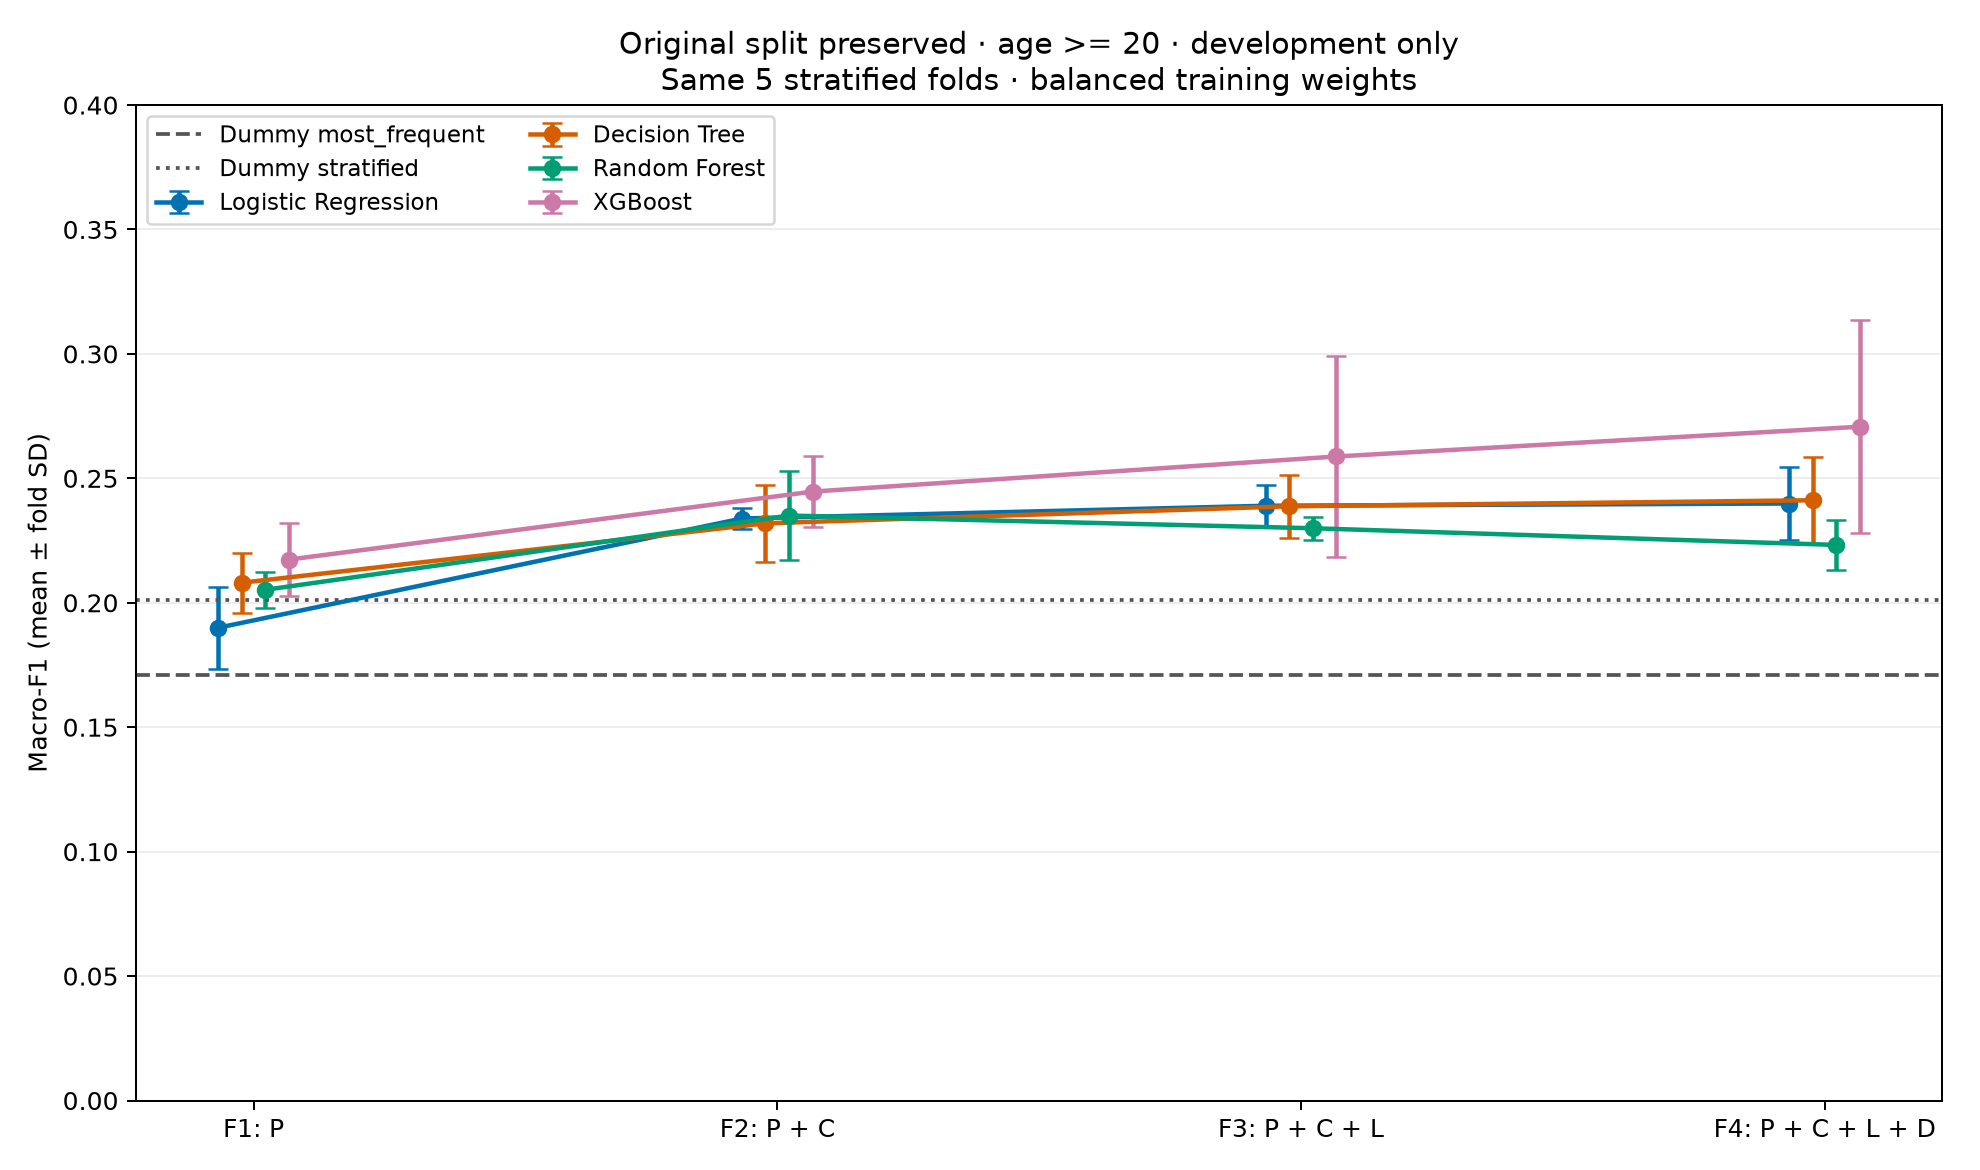
\includegraphics[width=0.9\textwidth]{figures/feature_group_comparison_final_protocol.png}
\label{fig:ablation-comparison}
\end{figure}

\subsection{Phân tích khoa học}
Từ kết quả Bảng \ref{tab:ablation-results}, một số phát hiện then chốt được rút ra:
\begin{enumerate}
    \item \textbf{Đóng góp rõ nét của nhóm Tiền sử bệnh lý lâm sàng ($F_1 \to F_2$):} Theo phân chia nhóm đặc trưng chính thức, nhóm $F_1$ (10 biến) đã bao gồm 5 chỉ số thể chất/sinh tồn và 5 xét nghiệm máu thiết yếu (HbA1c, Cholesterol, HDL, Creatinine, Albumin). Bước chuyển $F_1 \to F_2$ bổ sung 9 biến tiền sử bệnh lý mạn tính và chẩn đoán lâm sàng của bác sĩ (tăng huyết áp, đái tháo đường, 5 bệnh lý tim mạch/đột quỵ, ung thư và tự đánh giá sức khỏe), tạo ra mức tăng hiệu năng rõ nét nhất trên toàn bộ các mô hình: Macro-F1 của Hồi quy Logistic tăng từ 0.1900 lên 0.2338 (+23.1\%), Random Forest tăng từ 0.2052 lên 0.2350 (+14.5\%), và XGBoost tăng từ 0.2173 lên 0.2447 (+12.6\%). Điều này xác nhận giả thuyết y sinh rằng tiền sử bệnh mạn tính cung cấp tín hiệu bổ sung giá trị cho các chỉ số hóa sinh máu.
    \item \textbf{Đóng góp của nhóm Lối sống và Nhân khẩu học ($F_3, F_4$):} Nhóm đặc trưng lối sống (giấc ngủ, vận động thể lực, hút thuốc, sử dụng rượu bia) và nhân khẩu học (tuổi, giới tính, học vấn, tỷ lệ nghèo) tiếp tục nâng hiệu năng của XGBoost lên mức Macro-F1 = \textbf{0.2707 $\pm$ 0.0428} (Balanced Accuracy = 0.2837 $\pm$ 0.0485). Đối với Random Forest chưa tinh chỉnh, việc tăng từ 19 lên 34 đặc trưng khiến Macro-F1 giảm nhẹ (từ 0.2350 xuống 0.2232 $\pm$ 0.0099), do việc lấy mẫu ngẫu nhiên $\sqrt{d}$ đặc trưng tại mỗi nhánh bị phân tán bởi các biến tương quan yếu, đặt ra yêu cầu phải tinh chỉnh siêu tham số có kiểm soát.
    \item \textbf{Sự khác biệt giữa Weighted-F1 và Macro-F1:} Weighted-F1 luôn đạt giá trị rất cao (từ 0.49 đến 0.67) do bị chi phối bởi lớp đa số $C_0$ (chiếm ~75\%). Ngược lại, Macro-F1 dao động quanh mức 0.19 -- 0.27, phản ánh trung thực thách thức trong việc nhận diện các mức độ triệu chứng thiểu số ($C_2, C_3, C_4$).
\end{enumerate}

\subsection{Kết nối phương pháp luận: Từ lựa chọn đặc trưng đến tối ưu hóa mô hình}
Kết quả Feature Ablation khẳng định rằng không gian đặc trưng đầy đủ $F_4$ mang lại tiềm năng biểu diễn tốt nhất, song các mô hình với siêu tham số mặc định chưa khai thác triệt để tiềm năng này do hiện tượng phân tán ngẫu nhiên và mất cân bằng lớp. Do đó, bước tiếp theo là tối ưu hóa có hệ thống các siêu tham số mô hình thông qua quy trình kiểm định lồng nhau (Nested CV) khắt khe nhằm tìm ra cấu hình đường cơ sở tối ưu, đồng thời kiểm tra khả năng cải thiện thông qua các kỹ thuật học kết hợp (Ensemble Learning).

\FloatBarrier
\section{Tinh chỉnh siêu tham số và Mô hình học kết hợp}
\label{sec:tuning-va-ensemble}

\subsection{Tinh chỉnh Nested Cross-Validation}
Để lựa chọn cấu hình mô hình tối ưu một cách khách quan nhất và ngăn ngừa hiện tượng quá lạc quan trong đánh giá (optimistic bias), nghiên cứu áp dụng quy trình kiểm định lồng nhau (Nested CV) \cite{varma2006bias}:
\begin{itemize}
    \item \textbf{Outer CV (5 folds):} Đánh giá hiệu năng tổng quát hóa khách quan.
    \item \textbf{Inner CV (3 folds trên Outer Training):} Thực hiện \texttt{RandomizedSearchCV} với 12 cấu hình siêu tham số ngẫu nhiên cho mỗi ứng viên trên độ đo Macro-F1.
\end{itemize}

Bốn ứng viên được đưa vào Nested Tuning gồm: \texttt{LR/F4}, \texttt{RF/F4}, \texttt{XGB/F3} và \texttt{XGB/F4}. Kết quả Nested CV (trích xuất từ \texttt{results/nested\_cv\_tuning\_report.md}):
\begin{itemize}
    \item \texttt{LR/F4}: Macro-F1 outer đạt $0.2407 \pm 0.0173$.
    \item \texttt{XGB/F3}: Macro-F1 outer đạt $0.2516 \pm 0.0267$.
    \item \texttt{XGB/F4}: Macro-F1 outer đạt $0.2621 \pm 0.0353$.
    \item \textbf{\texttt{RF/F4} (Dẫn đầu):} Macro-F1 outer đạt \textbf{0.2755 $\pm$ 0.0270} (tăng +0.0523 so với baseline RF chưa tinh chỉnh).
\end{itemize}

Bộ siêu tham số tối ưu của Random Forest trên toàn bộ tập Development: \texttt{n\_estimators = 150}, \texttt{max\_depth = 8}, \texttt{max\_features = 0.5}, \texttt{min\_samples\_split = 10}, \texttt{min\_samples\_leaf = 8}, \texttt{class\_weight = 'balanced\_subsample'}, \texttt{criterion = 'gini'}. Cấu hình này được khóa chính thức thành \textbf{Frozen Random Forest Spec} trong file cấu hình \texttt{artifacts/final\_model\_spec.json}.

\subsection{Thực nghiệm Mô hình học kết hợp (Ensemble Study)}
Nghiên cứu tiếp tục kiểm tra xem liệu việc kết hợp các mô hình (Soft Voting và Stacking) có mang lại lợi ích thực sự so với mô hình Random Forest đơn nhất hay không. Kết quả từ \texttt{results/tables/ensemble\_results.csv}:
\begin{itemize}
    \item \texttt{Frozen Random Forest (Single)}: Macro-F1 = \textbf{0.2741 $\pm$ 0.0252}, Balanced Accuracy = \textbf{0.3015 $\pm$ 0.0294}.
    \item \texttt{Soft Voting (RF + XGBoost)}: Macro-F1 = 0.2748 $\pm$ 0.0248 (chỉ tăng không đáng kể +0.0007).
    \item \texttt{Stacking Classifier (Meta-LR)}: Macro-F1 = 0.2585 $\pm$ 0.0226 (suy giảm -0.0156).
\end{itemize}

Theo quy tắc ra quyết định thận trọng (Conservative Selection Rule) đã cam kết trong đề tài: \textit{Một mô hình phức tạp hơn chỉ được chấp nhận nếu cải thiện Macro-F1 ít nhất +0.01 và thắng ít nhất 4/5 folds}. Soft Voting và Stacking đều không thỏa mãn tiêu chí này. Do đó, nghiên cứu quyết định giữ nguyên \textbf{Random Forest đã tinh chỉnh làm mô hình chuẩn tắc duy nhất}, đảm bảo sự tinh gọn và khả năng kiểm soát thuật toán cao nhất.

\subsection{Kết nối phương pháp luận: Từ mô hình tối ưu đến khảo sát độ chi tiết nhãn}
Sau khi xác lập mô hình Frozen Random Forest trên không gian đặc trưng $F_4$ làm đường cơ sở chuẩn tắc, một câu hỏi phương pháp luận nền tảng được đặt ra: Tại sao hiệu năng phân loại 5 lớp ($T_5$) lại dừng lại ở mức Macro-F1 $\approx 0.27$? Liệu nguyên nhân nằm ở bản thân kiến trúc mô hình hay xuất phát từ cấu trúc phân phối nội tại của các mức độ triệu chứng PHQ-9? Để giải đáp câu hỏi này, Mục \ref{sec:target-granularity} tiến hành khảo sát sự suy thoái hiệu năng trên các mức độ chi tiết nhãn từ $T_2$ đến $T_5$.

\FloatBarrier
\section{Phân tích độ chi tiết nhãn mục tiêu ($T_2 \to T_5$)}
\label{sec:target-granularity}

\subsection{Mục tiêu và kết quả thực nghiệm}
Đây là một trong những phát hiện phương pháp luận trọng tâm nhất của đề tài, nhằm giải quyết câu hỏi \textbf{RQ2}: Lượng hóa quy luật suy giảm hiệu năng khi bài toán chuyển đổi từ phân loại nhị phân thô ($T_2$) sang các mức độ chi tiết ($T_3, T_4, T_5$) trên cùng một mô hình Frozen Random Forest và không gian đặc trưng $F_4$ ($N = 4.045$).

Kết quả thực nghiệm out-of-fold được đối chiếu từ \texttt{results/final\_report\_granularity.md} và trình bày trong Bảng \ref{tab:granularity-results}. Hình \ref{fig:granularity-curves} minh họa trực quan sự suy giảm này.

\begin{table}{Hiệu năng mô hình Random Forest theo độ chi tiết nhãn mục tiêu ($T_2 \to T_5$) trên Legacy Development ($N = 4.045$)}
\centering
\small
\label{tab:granularity-results}
\begin{tabular}{l c c c c c}
\toprule
\textbf{Nhiệm vụ} & \textbf{Số lớp} & \textbf{Độ chính xác (Acc)} & \textbf{Macro-F1 (Mean $\pm$ SD)} & \textbf{Balanced Acc} & \textbf{Weighted-F1} \\
\midrule
$T_2$ (Nhị phân: Không vs Có) & 2 & 74.24\% $\pm$ 1.26\% & \textbf{0.6639 $\pm$ 0.0113} & \textbf{0.6659 $\pm$ 0.0122} & 0.7436 $\pm$ 0.0100 \\
$T_3$ (3 nhóm: $C_0, C_1, C_2^+$) & 3 & 64.10\% $\pm$ 2.79\% & 0.4354 $\pm$ 0.0075 & 0.4667 $\pm$ 0.0101 & 0.6538 $\pm$ 0.0156 \\
$T_4$ (4 nhóm: $C_0, C_1, C_2, C_{3+4}$) & 4 & 61.06\% $\pm$ 2.58\% & 0.3380 $\pm$ 0.0177 & 0.3661 $\pm$ 0.0202 & 0.6351 $\pm$ 0.0169 \\
$T_5$ (5 mức chuẩn PHQ-9) & 5 & 61.38\% $\pm$ 2.03\% & 0.2630 $\pm$ 0.0222 & 0.2805 $\pm$ 0.0199 & 0.6339 $\pm$ 0.0116 \\
\bottomrule
\end{tabular}
\end{table}


\begin{figure}{Đồ thị thể hiện sự suy giảm nghiêm trọng của Macro-F1 và Balanced Accuracy từ $T_2$ đến $T_5$}
\centering
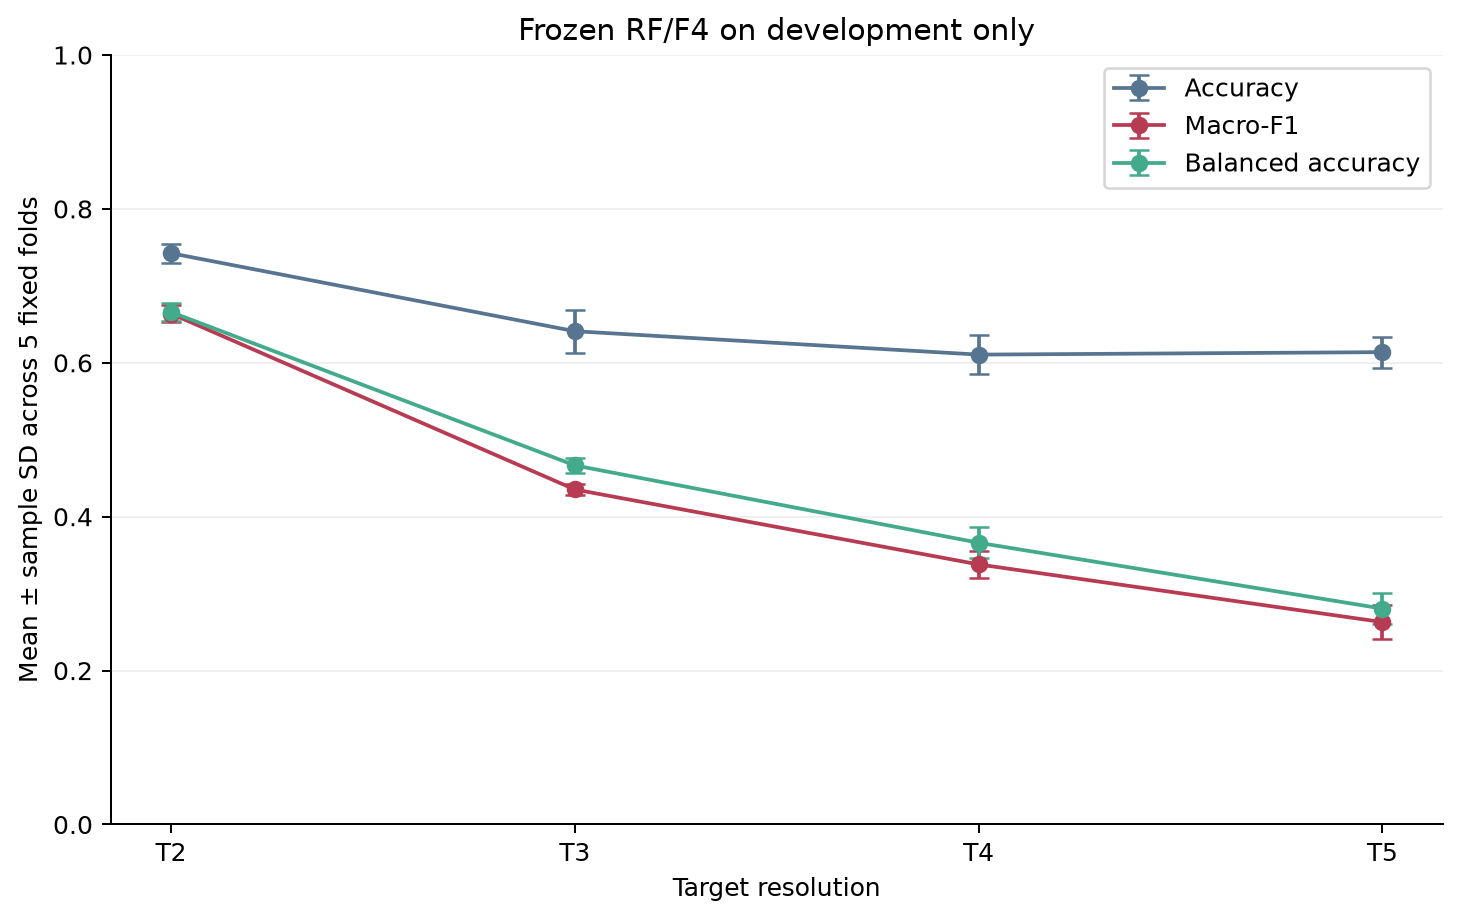
\includegraphics[width=0.85\textwidth]{figures/granularity_performance.png}
\label{fig:granularity-curves}
\end{figure}

\subsection{Phân tích nguyên nhân suy giảm và vị trí điểm nghẽn}
Từ Bảng \ref{tab:granularity-results}, sự sụt giảm hiệu năng giữa các bước chuyển đổi được lượng hóa:
\begin{itemize}
    \item \textbf{Bước chuyển $T_2 \to T_3$:} Macro-F1 sụt giảm tới \textbf{-0.2285} (từ 0.6639 xuống 0.4354, tương đương giảm 34.4\%). Đây là bước sụt giảm lớn nhất trong toàn bộ chuỗi thực nghiệm!
    \item \textbf{Bước chuyển $T_3 \to T_4$:} Macro-F1 giảm \textbf{-0.0974} (từ 0.4354 xuống 0.3380).
    \item \textbf{Bước chuyển $T_4 \to T_5$:} Macro-F1 giảm \textbf{-0.0750} (từ 0.3380 xuống 0.2630).
\end{itemize}

\textbf{Tại sao bước chuyển $T_2 \to T_3$ lại gây suy giảm mạnh nhất?}  
Trong nhiệm vụ nhị phân $T_2$, toàn bộ các đối tượng có triệu chứng từ nhẹ đến nặng ($s \ge 5$) được gộp chung thành một lớp dương tính. Mô hình chỉ cần phân tách giữa người hoàn toàn bình thường và người có bất kỳ dấu hiệu bất thường nào. Tuy nhiên, khi chuyển sang $T_3$, nhóm triệu chứng nhẹ ($C_1$: PHQ-9 từ 5 đến 9 điểm) bị tách ra thành một lớp riêng biệt nằm kẹp giữa $C_0$ và $C_2^+$. 

Phân tích ma trận nhầm lẫn của $T_3$ (Hình \ref{fig:granularity-t3-cm}) dựa trên kết quả kiểm định Out-of-fold thực tế (\texttt{results/tables/granularity\_oof\_predictions.csv}) cho thấy: Trong tổng số 638 bệnh nhân có triệu chứng nhẹ ($C_1$), có tới \textbf{347 mẫu (54.39\%)} bị mô hình nhầm lẫn thành $C_0$ (bình thường), \textbf{187 mẫu (29.31\%)} bị nhầm thành $C_2^+$ (nặng), và chỉ có \textbf{104 mẫu (16.30\%)} được phân loại chính xác vào lớp $C_1$. Độ nhạy (Recall) của lớp $C_1$ chỉ đạt vỏn vẹn \textbf{16.29\%}!

\begin{figure}{Ma trận nhầm lẫn Out-of-fold của nhiệm vụ 3 lớp $T_3$, chỉ ra điểm nghẽn nghiêm trọng tại lớp $C_1$}
\centering
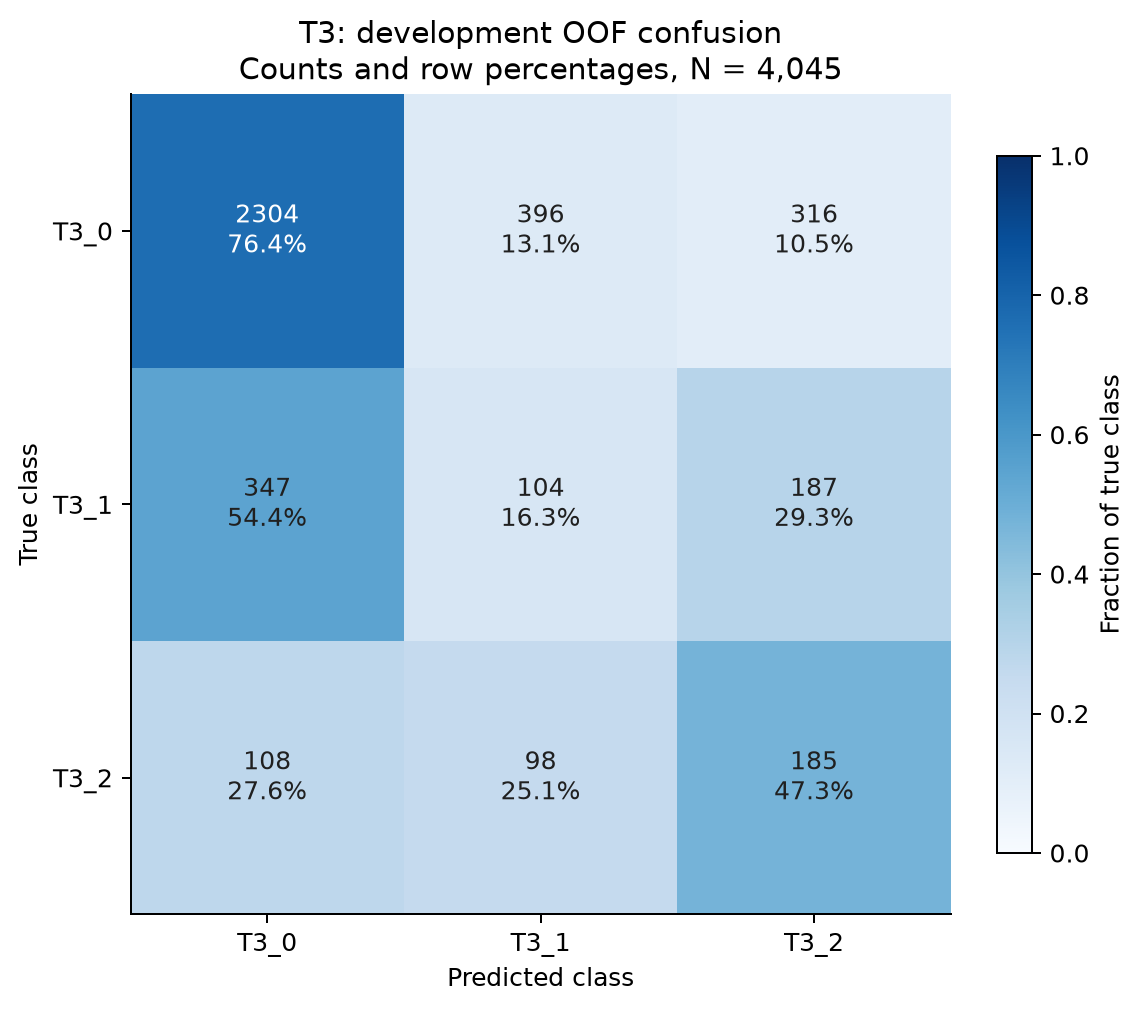
\includegraphics[width=0.65\textwidth]{figures/granularity_T3_confusion.png}
\label{fig:granularity-t3-cm}
\end{figure}

Phân tích thành phần chính (PCA) trên không gian đặc trưng sinh lý (Hình \ref{fig:overlap-pca}) cho thấy rõ: Các điểm dữ liệu của $C_0$ và $C_1$ chồng lấn gần như hoàn toàn lên nhau. Sự khác biệt về huyết áp, đường huyết hay mỡ máu giữa một người có 4 điểm PHQ-9 (xếp vào $C_0$) và một người có 5 điểm PHQ-9 (xếp vào $C_1$) là cực kỳ mong manh và không mang tính phân tách thống kê rõ rệt.

\begin{figure}{Trực quan hóa không gian đặc trưng bằng PCA: Sự chồng lấn phân phối sinh lý dày đặc giữa các mức độ triệu chứng}
\centering
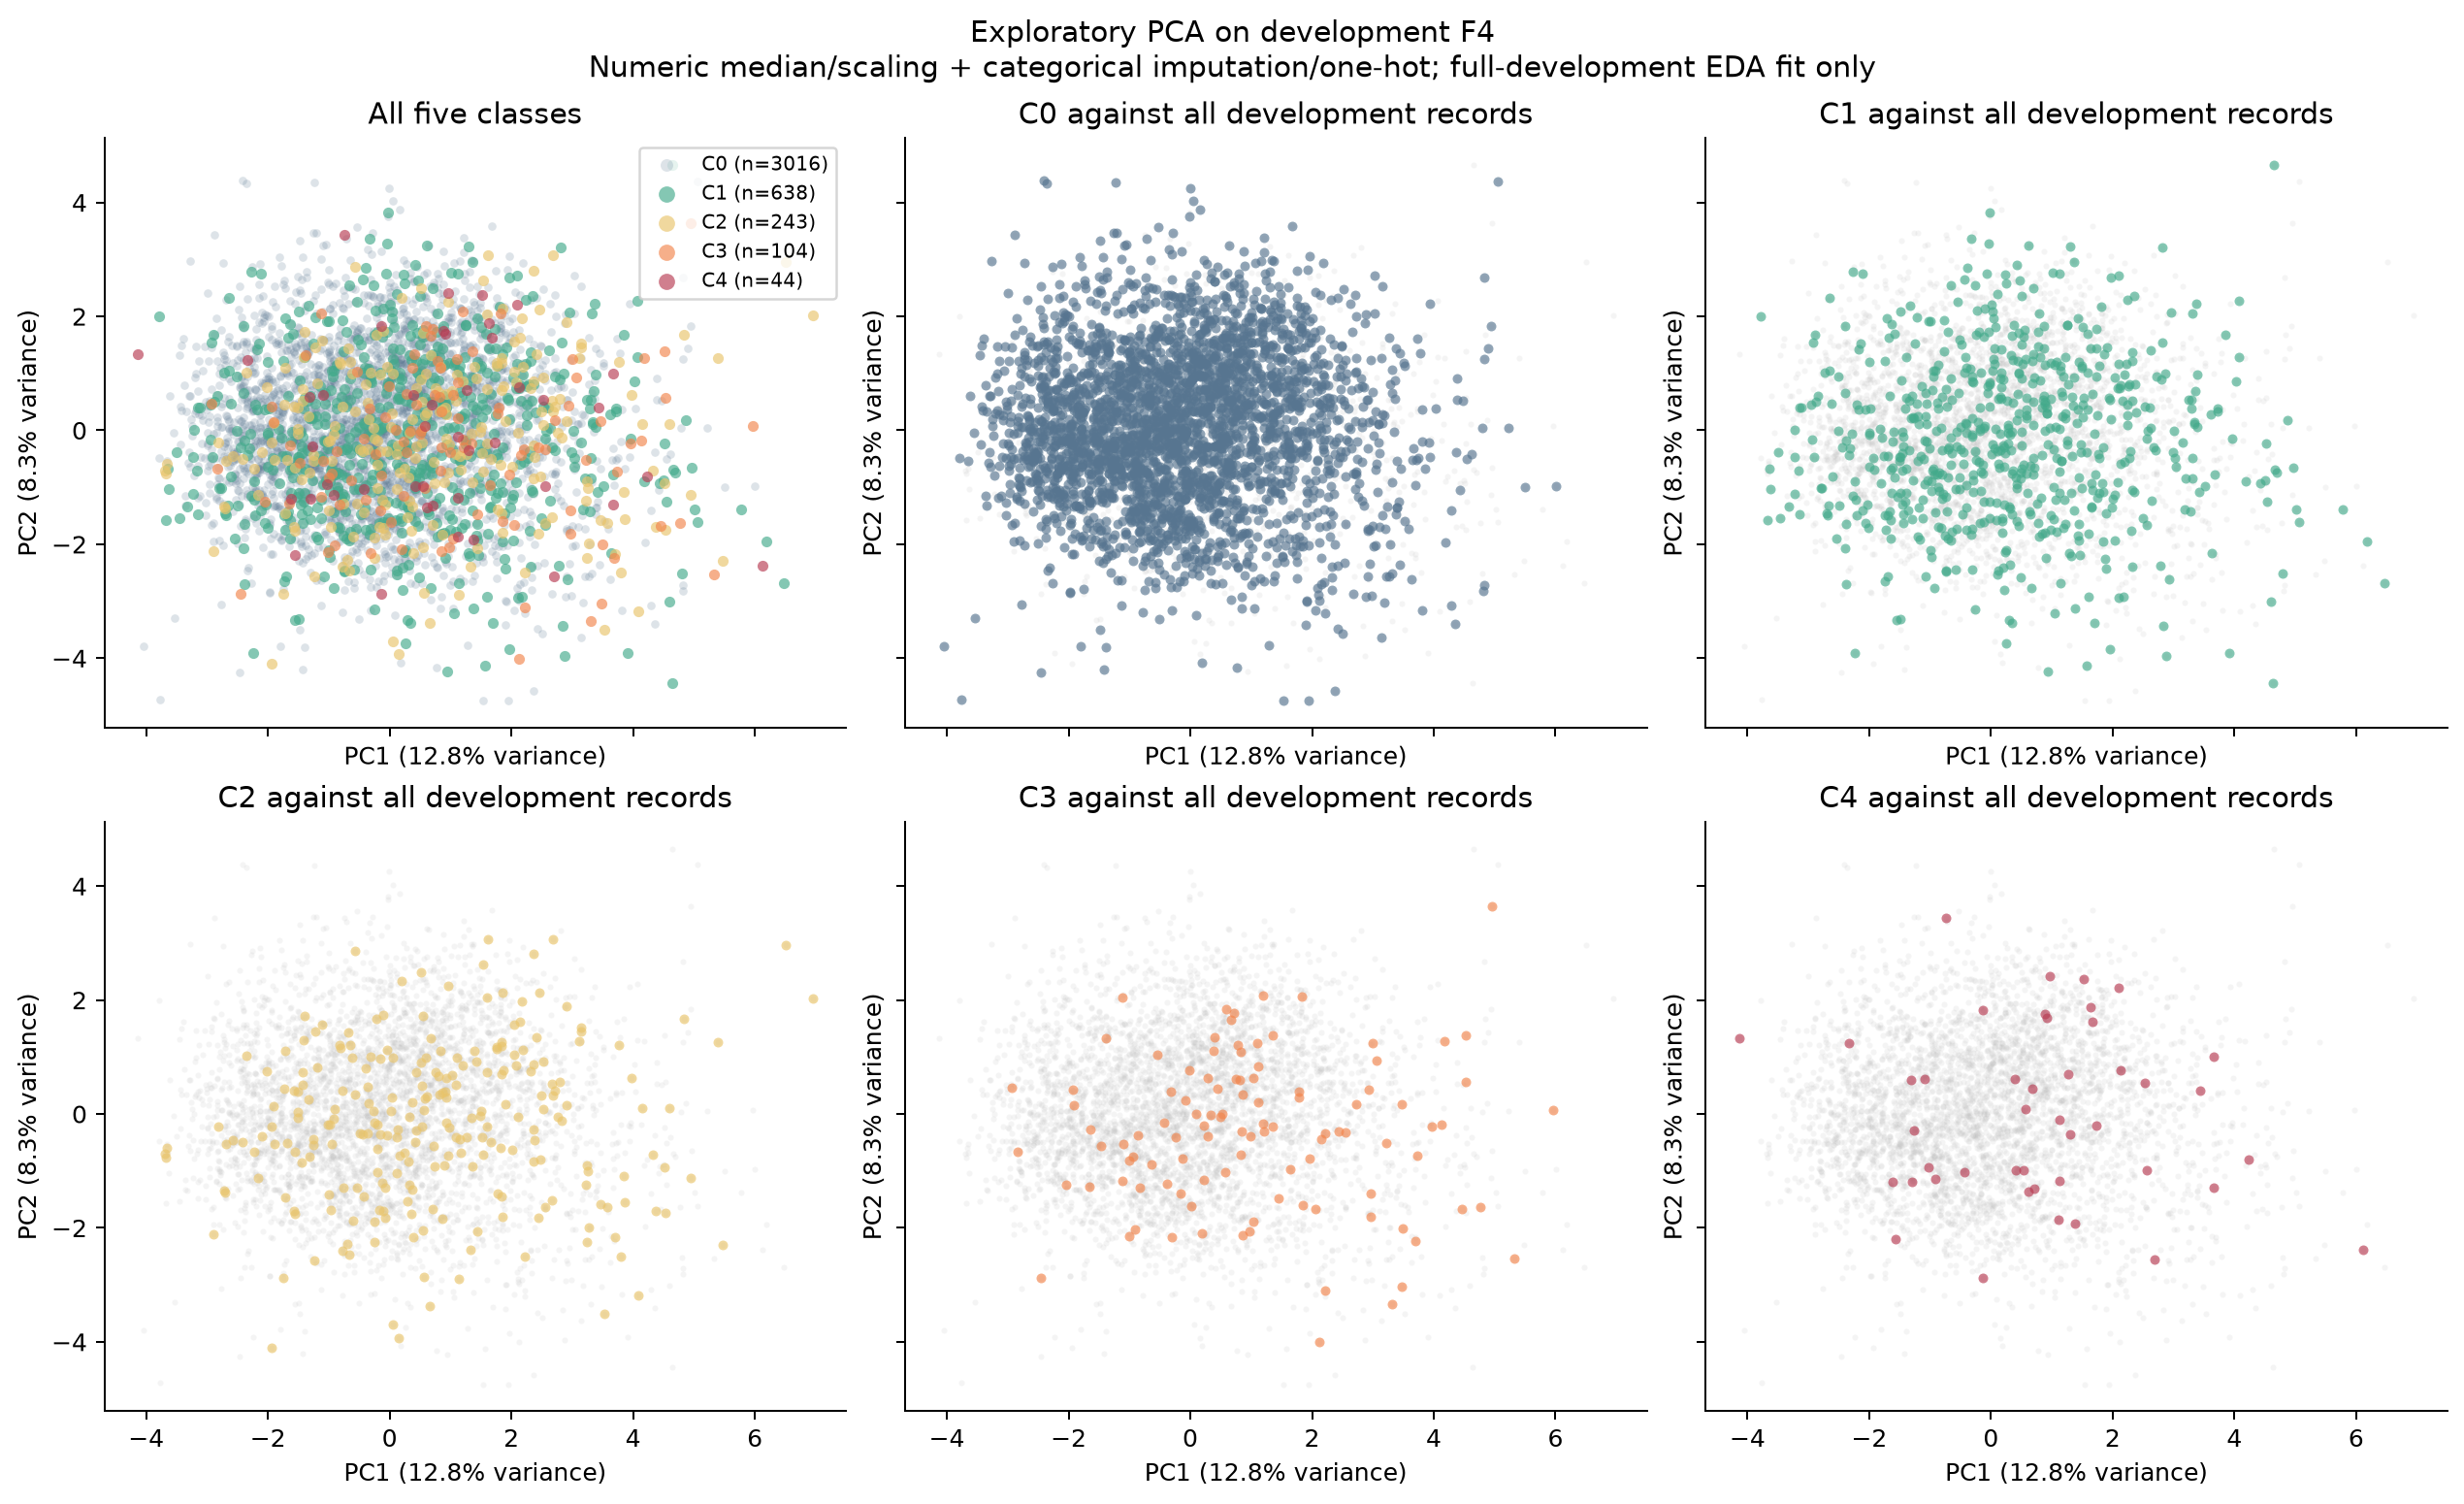
\includegraphics[width=0.95\textwidth]{figures/overlap_pca_C0_C4.png}
\label{fig:overlap-pca}
\end{figure}

\subsection{Kết nối phương pháp luận: Từ cỡ mẫu đơn chu kỳ đến khảo sát đa chu kỳ quy mô lớn}
Hiện tượng suy giảm hiệu năng nghiêm trọng tại bước chuyển $T_2 \to T_3$ và trần hiệu năng tại $T_5$ (Macro-F1 $\approx 0.26$) trên tập Legacy Cohort ($N = 4.045$) đặt ra một câu hỏi then chốt: Liệu hiện tượng này có phải do hạn chế về quy mô dữ liệu? Nếu tăng cỡ mẫu lên gấp 3 lần bằng cách gộp các chu kỳ NHANES tiếp theo ($N = 14.581$), liệu mô hình có vượt qua được ranh giới chồng lấn phân phối để cải thiện Macro-F1 hay không? Mục \ref{sec:thuc-nghiem-multicycle} sẽ kiểm chứng giả thuyết này thông qua thiết kế thực nghiệm đa chu kỳ có đối chứng.

\FloatBarrier
\section{Thực nghiệm Tổng quát hóa trên Multi-Cycle Cohort}
\label{sec:thuc-nghiem-multicycle}

Để trả lời câu hỏi nghiên cứu \textbf{RQ3}, framework DepSev-ML được mở rộng đánh giá trên tập dữ liệu đa chu kỳ chính thức với không gian đặc trưng hài hòa $F_{4\_\text{common31}}$ gồm 31 biến số. Bốn nhánh thực nghiệm có kiểm soát được thiết kế:
\begin{itemize}
    \item \textbf{Branch A (Single-cycle 2013--2014, $N = 5.054$):} Đóng vai trò là đối chứng chu kỳ đơn hợp lệ trong cùng không gian đặc trưng Common31.
    \item \textbf{Branch B (Pooled Multi-cycle 2011--2016, $N = 14.581$):} Gộp toàn bộ 3 chu kỳ để tăng cỡ mẫu lên gấp gần 3 lần.
    \item \textbf{Branch C (Matched-N, $N = 5.054$):} Lấy mẫu ngẫu nhiên từ tập Pooled sao cho cỡ mẫu đúng bằng Branch A nhằm cô lập tác động của quy mô mẫu khỏi thành phần chu kỳ.
    \item \textbf{Branch D (Temporal Evaluation):} Huấn luyện trên hai chu kỳ quá khứ 2011--2014 ($N = 9.693$), kiểm tra độc lập trên chu kỳ tương lai 2015--2016 ($N = 4.888$).
\end{itemize}

Kết quả thực nghiệm trên nhiệm vụ 5 lớp $T_5$ (trích xuất từ \texttt{results/final\_report\_integrated.md}):
\begin{itemize}
    \item \textbf{Macro-F1 không tăng khi gộp dữ liệu:} Branch A đạt Macro-F1 = \textbf{0.2634 $\pm$ 0.0152}, trong khi Branch B đạt Macro-F1 = \textbf{0.2619 $\pm$ 0.0098}. Sự khác biệt là hoàn toàn không đáng kể (-0.0015).
    \item \textbf{Balanced Accuracy cải thiện nhẹ:} Tăng từ \textbf{0.2841 $\pm$ 0.0142} (Branch A) lên \textbf{0.3076 $\pm$ 0.0118} (Branch B).
    \item \textbf{Recall của các lớp nặng hiếm mẫu ($C_3, C_4$) được cải thiện:} Khi số lượng mẫu $C_4$ trong tập huấn luyện tăng từ 55 lên 167 mẫu, độ nhạy Recall $C_4$ tăng từ 10.91\% lên 17.37\%. Tuy nhiên, độ chính xác dự đoán (Precision) của $C_4$ vẫn ở mức rất thấp (khoảng 3--5\%), do đó điểm F1 của các lớp này hầu như không thay đổi và không kéo tăng được Macro-F1 tổng thể.
    \item \textbf{Kiểm định thời gian (Branch D):} Trên tập dữ liệu độc lập NHANES 2015--2016 ($N = 4.888$ đối tượng, gồm đầy đủ tất cả mẫu hợp lệ mà không có bất kỳ mẫu nào bị loại bỏ), mô hình 5 lớp duy trì Macro-F1 = \textbf{0.2584} và Balanced Accuracy = \textbf{0.3012}, chứng minh mô hình không bị quá khớp theo thời gian nhưng sự hạn chế về khả năng phân tách đa mức vẫn tồn tại khách quan.

\end{itemize}

\textbf{Kết quả kiểm định theo dòng thời gian trên nhiệm vụ 3 lớp $T_3$:}  
Bảng \ref{tab:multicycle-temporal-results} tổng hợp hiệu năng của các mô hình $T_3$ trên tập kiểm định thời gian Branch D ($N = 4.888$). Kết quả cho thấy mô hình Ordinal Logistic Regression cân bằng ($E_{7a}$) tiếp tục duy trì Balanced Accuracy cao nhất (\textbf{0.5073}) và nhận diện được \textbf{59.30\%} số ca bệnh nặng $C_2^+$.

\begin{table}{Kết quả kiểm định tổng quát hóa theo dòng thời gian (Branch D, NHANES 2015--2016, $N = 4.888$)}
\centering
\small
\setlength{\tabcolsep}{4.5pt}
\label{tab:multicycle-temporal-results}
\begin{tabular}{l c c c c c c c}
\toprule
\textbf{Mô hình ($T_3$)} & \textbf{Macro-F1} & \textbf{BalAcc} & \textbf{Acc} & \textbf{Recall $C_0$} & \textbf{Recall $C_1$} & \textbf{Recall $C_2^+$} & \textbf{Class MAE} \\
\midrule
$E_0$ (Flat RF)                     & 0.4345 & 0.4908 & 62.68\% & 73.66\% & 18.79\% & 54.77\% & 0.5008 \\
$E_1$ (Hard RF--RF)                 & \textbf{0.4393} & 0.4879 & 66.35\% & 79.86\% & 14.51\% & 52.01\% & 0.4556 \\
$E_4$ (Soft RF--RF)                 & 0.4223 & 0.4594 & \textbf{71.91\%} & 90.60\% & 4.76\% & 42.46\% & \textbf{0.3766} \\
$E_5$ (Soft RF--LR)                 & 0.4265 & 0.4681 & 71.79\% & 90.08\% & 4.88\% & 45.48\% & 0.3801 \\
$E_{6b}$ (Soft Cost M2)             & 0.3439 & 0.4691 & 34.84\% & 26.94\% & \textbf{60.29\%} & 53.52\% & 0.7306 \\
$E_{7a}$ (OLR Balanced)             & 0.4349 & \textbf{0.5073} & 56.28\% & 61.74\% & 31.15\% & 59.30\% & 0.5503 \\
$E_{7b}$ (CumBin LR)                & 0.3632 & 0.4982 & 62.21\% & 75.23\% & 0.12\% & \textbf{74.12\%} & 0.5833 \\
$E_{7b}$ (CumBin RF)                & 0.3861 & 0.4861 & 67.88\% & 84.16\% & 0.36\% & 61.31\% & 0.4695 \\
\bottomrule
\end{tabular}
\end{table}


\textbf{Kết luận RQ3:} Việc mở rộng cỡ mẫu đa chu kỳ giúp mô hình ước lượng phân phối của các lớp hiếm ổn định hơn (tăng nhẹ Balanced Accuracy và Recall lớp nặng), nhưng không thể đảo ngược hoàn toàn sự suy giảm hiệu năng của bài toán phân loại đa mức nếu không gian đặc trưng sinh lý ngoại vi vẫn có độ chồng lấn phân phối cao.

\FloatBarrier
\section{Định hướng nghiên cứu mở rộng: Chuyển dịch mục tiêu sang Nhiệm vụ T3}
\label{sec:dinh-huong-t3}

\subsection{Cơ sở lý luận và Động lực chuyển đổi sang Nhiệm vụ T3}
Các phát hiện thực nghiệm từ Mục \ref{sec:target-granularity} và Mục \ref{sec:thuc-nghiem-multicycle} đã chỉ ra một rào cản mang tính bản chất: Trên nhiệm vụ 5 mức độ tiêu chuẩn ($T_5$), mô hình học máy đạt trần hiệu năng quanh mức Macro-F1 $\approx 0.26$, ngay cả khi quy mô tập dữ liệu được mở rộng lên 14.581 mẫu qua 3 chu kỳ NHANES liên tiếp. Nguyên nhân cốt lõi không nằm ở thuật toán hay dung lượng mẫu, mà xuất phát từ sự kết hợp giữa tỷ số mất cân bằng cực đoan ($\text{IR} \approx 68.5:1$) và mức độ chồng lấn phân phối sinh lý học dày đặc giữa các trạng thái lâm sàng kế cận (đặc biệt là giữa $C_0$ và $C_1$, cũng như giữa $C_2, C_3$ và $C_4$).

Trong bối cảnh y tế dự phòng và thực hành sàng lọc sức khỏe cộng đồng, mục tiêu ưu tiên hàng đầu không phải là phân định tuyệt đối giữa các mức độ cận kề (chẳng hạn phân biệt giữa mức Trầm cảm vừa và Nặng vừa), mà là \textbf{phân luồng can thiệp y tế (Clinical Triage)}:
\begin{enumerate}
    \item \textbf{Nhóm không có triệu chứng ($C_0$, $0 \le s \le 4$):} Chiếm đa số trong quần thể, không đòi hỏi can thiệp y tế.
    \item \textbf{Nhóm triệu chứng nhẹ ($C_1$, $5 \le s \le 9$):} Xuất hiện triệu chứng dưới ngưỡng chẩn đoán, cần được khuyến nghị điều chỉnh lối sống, giảm căng thẳng và theo dõi diễn tiến định kỳ.
    \item \textbf{Nhóm Nặng theo quy ước nghiên cứu ($C_2^+$, $10 \le s \le 27$):} Vượt qua ngưỡng cắt lâm sàng truyền thống ($s \ge 10$), bao gồm toàn bộ các đối tượng từ mức vừa đến rất nặng ($C_2 \cup C_3 \cup C_4$), là đối tượng bắt buộc phải được chuyển tuyến khám chuyên khoa tâm thần và can thiệp điều trị.
\end{enumerate}

Do đó, nghiên cứu tiến hành \textbf{chuyển dịch mục tiêu sang Nhiệm vụ 3 nhóm ($T_3$)} như một hướng nghiên cứu mở rộng có tính thực tiễn cao. 

\subsection{Làm rõ ranh giới phương pháp luận giữa T5 và T3}
Cần thiết lập một tuyên bố phương pháp luận rõ ràng nhằm tránh mọi ngộ nhận khoa học:
\begin{quote}
\textit{Tuyên bố nguyên tắc:} Việc chuyển dịch sang nhiệm vụ $T_3$ \textbf{không đồng nghĩa với việc giải quyết hay vượt qua trần hiệu năng của bài toán $T_5$}. Đây là hai bài toán với không gian nhãn hoàn toàn khác biệt ($|\mathcal{Y}| = 3$ so với $|\mathcal{Y}| = 5$), do đó các chỉ số hiệu năng (Macro-F1, Balanced Accuracy) giữa $T_3$ và $T_5$ không thể so sánh số học trực tiếp với nhau.
\end{quote}

Mục đích thực sự của việc tập trung vào nhiệm vụ $T_3$ là thiết lập một \textbf{môi trường thực nghiệm chuẩn mực (Benchmark Environment)} có ý nghĩa lâm sàng rõ rệt, từ đó đánh giá có hệ thống xem liệu các kiến trúc học máy nâng cao — bao gồm Phân loại phân cấp hai tầng cứng ($E_1 \to E_3$), Phân loại phân cấp mềm kết hợp Nhạy chi phí ($E_4 \to E_6$), và Phân loại thứ bậc ($E_7$) — có thể giải quyết được hiện tượng lan truyền sai số và bảo vệ an toàn cho nhóm bệnh nhân nặng ($C_2^+$) hay không.

\FloatBarrier
\section{Thực nghiệm $T_3$ – So sánh Phân loại Phẳng và Phân cấp Cứng}
\label{sec:thuc-nghiem-t3-hard}

Để tìm giải pháp kiến trúc khắc phục hiện tượng suy giảm hiệu năng trên không gian 3 lớp $T_3$ ($C_0, C_1, C_2^+$), nghiên cứu triển khai nhóm thực nghiệm Phân loại phân cấp hai tầng cứng ($E_1 \to E_3b$) đối chứng với mô hình Phân loại phẳng $E_0$ (Random Forest phẳng).

Các mô hình được đánh giá bao gồm:
\begin{itemize}
    \item \texttt{E0\_Flat\_RF}: Random Forest phân loại trực tiếp 3 lớp.
    \item \texttt{E1\_Hard\_RF\_RF}: Hard Hierarchical RF (Tầng 1) + RF (Tầng 2), ngưỡng cắt $\tau_1 = \tau_2 = 0.5$.
    \item \texttt{E2\_Hard\_Tuned}: Hard Hierarchical RF--RF với ngưỡng cắt được tối ưu hóa tương thích theo từng fold qua Inner CV ($\tau_1 \in [0.45, 0.50], \tau_2 \in [0.50, 0.55]$, trung bình $\tau_1 = 0.47, \tau_2 = 0.53$).
    \item \texttt{E3a\_Hard\_RF\_LR}: Hard Hierarchical RF (Tầng 1) + Hồi quy Logistic cân bằng (Tầng 2).
    \item \texttt{E3b\_Hard\_RF\_XGB}: Hard Hierarchical RF (Tầng 1) + XGBoost cân bằng (Tầng 2).
\end{itemize}

Kết quả thực nghiệm out-of-fold trên Legacy Development Cohort ($N = 4.045$) được tổng hợp trong Bảng \ref{tab:hard-hierarchical-results}.

\begin{table}{So sánh hiệu năng giữa Flat Classification và Hard Hierarchical trên nhiệm vụ $T_3$ ($N = 4.045$)}
\centering
\small
\label{tab:hard-hierarchical-results}
\begin{tabular}{l c c c c c c}
\toprule
\textbf{Mô hình} & \textbf{Macro-F1} & \textbf{BalAcc} & \textbf{Accuracy} & \textbf{Recall $C_1$} & \textbf{Recall $C_2^+$} & \textbf{Bỏ sót $C_2^+ \to C_0$} \\
\midrule
$E_0$ (Flat RF)       & 0.4354 $\pm$ 0.0075 & 0.4667 & 64.10\% & 16.29\% & 47.32\% & 108 ca \\
$E_1$ (Hard RF--RF)   & 0.4550 $\pm$ 0.0056 & 0.4745 & 68.08\% & 16.46\% & 43.74\% & 120 ca \\
$E_2$ (Hard Tuned)    & \textbf{0.4586 $\pm$ 0.0124} & 0.4745 & 65.32\% & \textbf{25.69\%} & 39.63\% & \textbf{95 ca} \\
$E_3a$ (Hard RF--LR)  & 0.4567 $\pm$ 0.0271 & \textbf{0.4964} & \textbf{68.43\%} & 11.75\% & \textbf{55.00\%} & 120 ca \\
$E_3b$ (Hard RF--XGB) & 0.4575 $\pm$ 0.0182 & 0.4790 & 68.23\% & 16.77\% & 44.76\% & 120 ca \\
\bottomrule
\end{tabular}
\end{table}


\textbf{Phân tích chuyên sâu về hiệu năng và Lan truyền sai số của Hard Routing:}
\begin{enumerate}
    \item \textbf{Ưu thế ổn định của $E_1$ so với $E_0$ qua các Folds:} Đối chiếu kết quả kiểm định chéo từng fold (\texttt{experiments/hierarchical\_t3/outputs/fold\_metrics.csv}) cho thấy mô hình Hard Hierarchical $E_1$ đạt Macro-F1 cao hơn Flat RF $E_0$ trên \textbf{cả 5/5 folds} (Fold 1: +0.0105; Fold 2: +0.0181; Fold 3: +0.0151; Fold 4: +0.0219; Fold 5: +0.0326), nâng Macro-F1 trung bình từ 0.4354 lên 0.4550 $\pm$ 0.0056.
    \item \textbf{Làm rõ bản chất độ chính xác Giai đoạn 2 (Routed vs Oracle vs End-to-end):} Để tránh hiểu nhầm số liệu thực nghiệm, cần phân biệt rõ ba góc độ đánh giá của bộ phân loại Tầng 2 (\texttt{experiments/hierarchical\_t3/outputs/stage\_metrics.csv}):
    \begin{itemize}
        \item \textit{Routed Evaluation (Độ chính xác thực tế trên luồng điều hướng):} Đạt trung bình \textbf{52.72\%}. Mẫu số của độ đo này là các mẫu được Tầng 1 dự đoán là có triệu chứng (bao gồm cả các ca dương tính thật và các ca báo động nhầm $C_0 \to \text{Symptomatic}$).
        \item \textit{Oracle Evaluation (Độ chính xác lý thuyết nếu Tầng 1 hoàn hảo):} Đạt Balanced Accuracy \textbf{58.69\%}. Đánh giá trên tập mẫu thực sự có triệu chứng ($C_1 \cup C_2^+$, $N = 1.029$).
        \item \textit{End-to-end Evaluation (Độ chính xác toàn hệ thống 3 lớp):} Mô hình $E_1$ đạt \textbf{68.08\%} trên toàn bộ $N = 4.045$ đối tượng.
    \end{itemize}
    \item \textbf{Khiếm khuyết tắc nghẽn lâm sàng của cổng cứng:} Tại Giai đoạn 1, cổng phân loại nhị phân cứng với ngưỡng $\tau_1 = 0.5$ đã loại bỏ nhầm \textbf{120 bệnh nhân thuộc nhóm Nặng quy ước ($C_2^+$)} (chiếm tới 30.7\% tổng số 391 bệnh nhân nặng). Những bệnh nhân này bị dán nhãn ngay lập tức là $C_0$ (bình thường) và không bao giờ có cơ hội được Giai đoạn 2 xem xét. Đây là minh chứng thực nghiệm điển hình cho hiện tượng lan truyền sai số một chiều trong kiến trúc phân cấp cứng.
\end{enumerate}

\subsection{Kết nối phương pháp luận: Từ hạn chế của cổng cứng đến định tuyến mềm}
Sự thất thoát 120 bệnh nhân nặng tại Giai đoạn 1 của mô hình Hard Hierarchical cho thấy ranh giới quyết định nhị phân cứng ($\tau_1 = 0.5$) là nguyên nhân trực tiếp dẫn tới hiện tượng lan truyền sai số một chiều. Để khắc phục điểm nghẽn này, phương pháp luận cần chuyển đổi từ việc ra quyết định rời rạc sang việc bảo toàn phân phối xác suất liên tục trên toàn bộ không gian mẫu (Soft Probability Fusion), đồng thời kết hợp cơ chế phạt lỗi bất đối xứng để bảo vệ các ca bệnh nặng. Mục \ref{sec:thuc-nghiem-soft-cost} sẽ triển khai nhóm thực nghiệm này.

\FloatBarrier
\section{Thực nghiệm Soft Hierarchical và Quyết định Nhạy chi phí ($E_4 \to E_6$)}
\label{sec:thuc-nghiem-soft-cost}

Để khắc phục hiện tượng tắc nghẽn của cổng cứng, nhóm thực nghiệm $E_4 \to E_6b$ được triển khai:
\begin{itemize}
    \item \texttt{$E\_4$ (Soft RF--RF)}: Tích hợp xác suất toàn phần, ra quyết định bằng Argmax.
    \item \texttt{$E\_5$ (Soft RF--LR)}: Tích hợp xác suất toàn phần với Tầng 2 là Logistic Regression, ra quyết định bằng Argmax.
    \item \texttt{$E\_6a$ (Soft RF--RF + Cost M1)}: Tối ưu hóa rủi ro Bayes với ma trận chi phí lâm sàng $M_1$.
    \item \texttt{$E\_6b$ (Soft RF--LR + Cost M1)}: Tối ưu hóa rủi ro Bayes với ma trận chi phí $M_1$.
\end{itemize}

Kết quả thực nghiệm out-of-fold trên Legacy Development Cohort ($N = 4.045$) được trình bày trong Bảng \ref{tab:soft-cost-results}. Hình \ref{fig:cost-curve} thể hiện đường cong đánh đổi chi phí khi tăng mức phạt qua các ma trận $M_0 \to M_3$.

\begin{table}{Hiệu năng mô hình Soft Hierarchical và Quyết định Nhạy chi phí trên nhiệm vụ $T_3$ ($N = 4.045$)}
\centering
\small
\setlength{\tabcolsep}{4.5pt}
\label{tab:soft-cost-results}
\begin{tabular}{l c c c c c c c}
\toprule
\textbf{Mô hình} & \textbf{Macro-F1} & \textbf{BalAcc} & \textbf{Acc} & \textbf{Rec $C_1$} & \textbf{Rec $C_2^+$} & \textbf{$C_2^+ \to C_0$} & \textbf{$C_0 \to C_2^+$} \\
\midrule
$E_4$ (Soft RF--RF Argmax) & 0.4206 $\pm$ 0.0104 & 0.4309 & \textbf{73.75\%} & 5.18\% & 30.19\% & 227 ca & \textbf{139 ca} \\
$E_5$ (Soft RF--LR Argmax) & 0.4270 $\pm$ 0.0118 & 0.4506 & 73.37\% & 3.45\% & 39.13\% & 211 ca & 176 ca \\
$E_{6a}$ (Soft Cost RF--RF) & \textbf{0.4535 $\pm$ 0.0149} & 0.4904 & 56.91\% & \textbf{40.92\%} & 44.25\% & \textbf{62 ca} & 215 ca \\
$E_{6b}$ (Soft Cost RF--LR) & 0.4521 $\pm$ 0.0190 & \textbf{0.5025} & 56.84\% & 34.64\% & \textbf{54.23\%} & \textbf{62 ca} & 294 ca \\
\bottomrule
\end{tabular}
\end{table}


\begin{figure}{Đường cong đánh đổi giữa việc giảm số ca bỏ sót nặng ($C_2^+ \to C_0$) và sự gia tăng cảnh báo giả ($C_0 \to C_2^+$) qua các ma trận chi phí $M_0 \to M_3$}
\centering
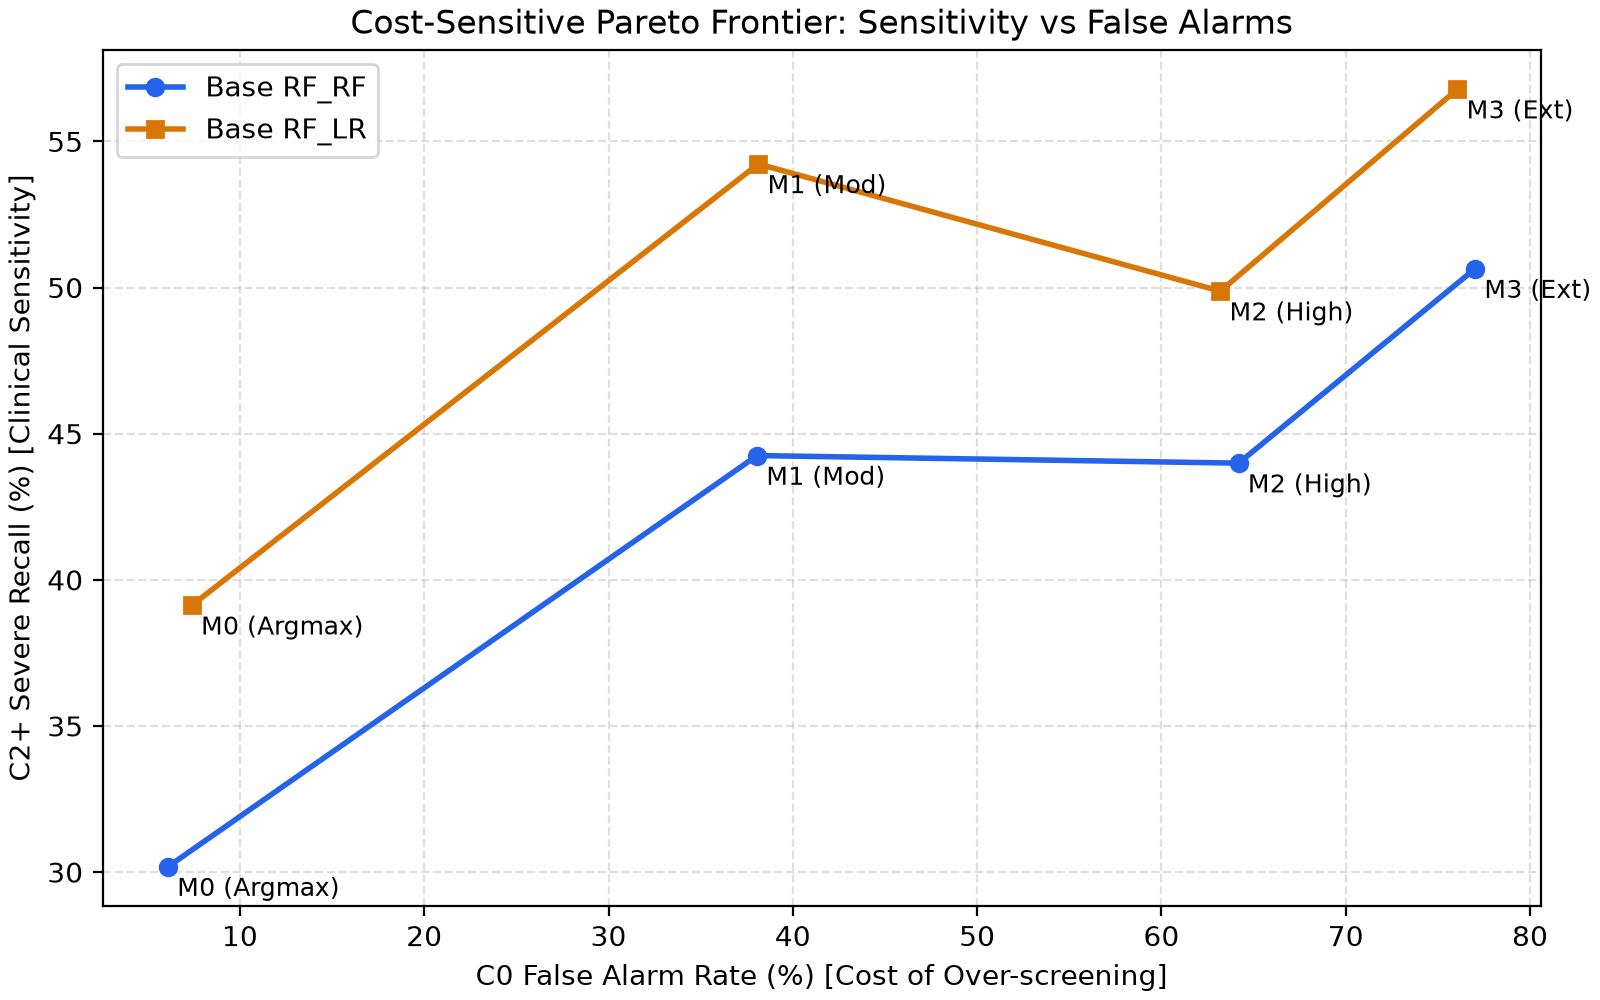
\includegraphics[width=0.85\textwidth]{figures/cost_tradeoff_curve.png}
\label{fig:cost-curve}
\end{figure}

\textbf{Phân tích khoa học:}
1. \textbf{Hạn chế của Soft Argmax ($E_4, E_5$):} Khi chỉ dùng Argmax xác suất mà không có ma trận chi phí, mô hình bị thiên lệch cực mạnh về lớp đa số $C_0$ (Recall $C_0 > 92\%$, nhưng Recall $C_1 < 5.2\%$). Số ca nặng $C_2^+$ bị bỏ sót thành $C_0$ tăng vọt lên \textbf{211 ca} ($E_5$) và \textbf{227 ca} ($E_4$).  
2. \textbf{Hiệu quả kiểm soát ca bỏ sót của Ma trận chi phí lâm sàng $M_1$ ($E_{6a}, E_{6b}$):} Khi áp dụng quy tắc rủi ro Bayes với ma trận $M_1$, cả hai mô hình $E_{6a}$ (RF--RF) và $E_{6b}$ (RF--LR) đều kéo giảm số ca bỏ sót nguy hiểm $C_2^+ \to C_0$ xuống chỉ còn đúng \textbf{62 ca} (giảm hơn 70\% so với mô hình Soft không trọng số). Đặc biệt, mô hình $E_{6a}$ đạt Recall lớp nhẹ $C_1$ lên tới \textbf{40.92\%} (mức cao nhất trong toàn bộ các mô hình thực nghiệm), trong khi $E_{6b}$ đạt Recall lớp nặng $C_2^+$ lên tới \textbf{54.23\%} và Balanced Accuracy đạt \textbf{0.5025}.
3. \textbf{Cảnh báo về sự đánh đổi khi tăng phạt cực đoan ($M_2, M_3$):} Nếu tiếp tục tăng mức phạt qua $M_2$ và $M_3$, số ca $C_2^+ \to C_0$ có thể giảm xuống 19 và 7 ca, nhưng số ca cảnh báo giả $C_0 \to C_2^+$ sẽ bùng nổ lên tới 1.906 và 2.294 ca, phá hủy hoàn toàn độ đặc hiệu của hệ thống sàng lọc. Do đó $M_1$ là điểm cân bằng tối ưu duy nhất.

\subsection{Kết nối phương pháp luận: Từ ma trận chi phí đến mô hình hóa thứ bậc}
Mặc dù mô hình Soft Cost-Sensitive ($E_{6a}, E_{6b}$) đã kéo giảm thành công số ca bỏ sót nặng từ 120 xuống 62 ca, bản chất của phương pháp này vẫn xem 3 lớp như các nhãn danh nghĩa rời rạc và chỉ can thiệp bằng ma trận phạt chi phí ở khâu hậu xử lý xác suất. Trong khi đó, các mức độ PHQ-9 vốn có quan hệ thứ tự tự nhiên nghiêm ngặt ($C_0 \prec C_1 \prec C_2^+$). Câu hỏi đặt ra là: Liệu việc tích hợp trực tiếp quan hệ thứ tự này ngay từ hàm mục tiêu huấn luyện thông qua các mô hình Phân loại thứ bậc (Ordinal Classification) có mang lại giải pháp căn cơ và thanh lịch hơn hay không? Mục \ref{sec:thuc-nghiem-ordinal} sẽ khảo sát nhóm thực nghiệm $E_7$.

\FloatBarrier
\section{Thực nghiệm Phân loại Thứ bậc (Ordinal Classification -- $E_7$)}
\label{sec:thuc-nghiem-ordinal}

\subsection{Mục tiêu và các mô hình thử nghiệm}
Thực nghiệm $E_7$ nhằm trả lời câu hỏi cốt lõi: Khai thác trực tiếp thứ tự tự nhiên $C_0 \prec C_1 \prec C_2^+$ thông qua các mô hình Ordinal Classification có mang lại hiệu năng vượt trội và giải quyết được sự đánh đổi giữa các chỉ số hay không. Bốn mô hình được đánh giá:
\begin{itemize}
    \item \texttt{E7a\_Ordinal\_LogReg}: Mô hình Proportional Odds Cumulative Logit, không dùng trọng số.
    \item \texttt{E7a\_Ordinal\_LogReg\_Balanced}: Mô hình Proportional Odds với \texttt{class\_weight="balanced"}.
    \item \texttt{E7b\_CumBin\_LR}: Mô hình Frank \& Hall với bộ phân loại cơ sở là Logistic Regression.
    \item \texttt{E7b\_CumBin\_RF}: Mô hình Frank \& Hall với bộ phân loại cơ sở là Random Forest.
\end{itemize}

Kết quả thực nghiệm out-of-fold chi tiết trên Legacy Development ($N = 4.045$) được trình bày trong Bảng \ref{tab:ordinal-results}.

\begin{table}{Kết quả thực nghiệm các mô hình Ordinal Classification trên nhiệm vụ $T_3$ ($N = 4.045$)}
\centering
\small
\setlength{\tabcolsep}{4.5pt}
\label{tab:ordinal-results}
\begin{tabular}{l c c c c c c c}
\toprule
\textbf{Mô hình} & \textbf{Macro-F1} & \textbf{BalAcc} & \textbf{Accuracy} & \textbf{Class MAE} & \textbf{QWK} & \textbf{Recall $C_1$} & \textbf{Recall $C_2^+$} \\
\midrule
$E_{7a}$ (OLR Unweighted) & 0.3846 & 0.4002 & \textbf{75.23\%} & \textbf{0.3377} & 0.2298 & 0.00\% & 22.00\% \\
$E_{7a}$ (OLR Balanced)   & \textbf{0.4518} & \textbf{0.5151} & 56.69\% & 0.5382 & 0.3398 & \textbf{32.93\%} & 60.37\% \\
$E_{7b}$ (CumBin LR)      & 0.3761 & 0.4949 & 63.41\% & 0.5718 & 0.2958 & 0.00\% & \textbf{72.88\%} \\
$E_{7b}$ (CumBin RF)      & 0.4191 & 0.4900 & 72.34\% & 0.3953 & \textbf{0.3744} & 0.16\% & 57.30\% \\
\bottomrule
\end{tabular}
\end{table}


\subsection{Phân tích hiện tượng suy biến lớp trung gian và vi phạm đơn điệu}
Thực nghiệm $E_7$ mang lại hai phát hiện khoa học đặc biệt quan trọng:

\textbf{1. Nghịch lý của Class MAE trong E7a không trọng số:}  
Mô hình \texttt{E7a} không trọng số đạt \textbf{Class MAE thấp nhất (0.3377)} và \textbf{Accuracy cao nhất (75.23\%)} trong toàn bộ các mô hình của dự án. Tuy nhiên, mô hình hoàn toàn không nhận diện được bất kỳ mẫu nào thuộc lớp $C_1$ (\textbf{Recall $C_1 = 0.00\%$}).  
*Làm rõ cơ chế tối ưu hóa:* Về mặt toán học, mô hình $E_{7a}$ tối ưu hóa hàm Negative Log-Likelihood với điều chuẩn $L_2$ trên các trọng số $\mathbf{w}$ (Negative Log-Likelihood của mô hình logit tích lũy), chứ không phải tối thiểu hóa trực tiếp Class MAE trong quá trình huấn luyện. Class MAE là chỉ số đánh giá hình học hậu kỳ. Dưới hiện tượng mất cân bằng lớp cực đoan (lớp $C_0$ chiếm ~75\%), nghiệm cực đại hợp lý (Maximum Likelihood) tự nhiên đẩy các ngưỡng cắt $\theta_0, \theta_1$ sao cho xác suất tích lũy dồn phần lớn về lớp đa số $C_0$. Khi đó, 74.5\% mẫu có khoảng cách lỗi bằng 0, 15.8\% mẫu $C_1$ chỉ chịu lỗi bằng 1, và 9.7\% mẫu $C_2^+$ chịu lỗi bằng 2, dẫn tới giá trị kỳ vọng của Class MAE hậu kỳ đạt mức rất thấp. Điều này chứng minh rằng: \textbf{Chỉ dựa vào Class MAE thấp để kết luận mô hình thứ bậc tốt là một sai lầm nghiêm trọng trên dữ liệu y tế mất cân bằng nếu không kiểm tra độ nhạy từng lớp.}

\textbf{2. Sự suy giảm nghiêm trọng của phương pháp Frank \& Hall (E7b):}  
Do hai bộ phân loại nhị phân $P(Y \ge 1)$ và $P(Y \ge 2)$ được huấn luyện độc lập, các siêu phẳng quyết định bị cắt nhau trong không gian đặc trưng. Thống kê out-of-fold ghi nhận \textbf{19.53\% số mẫu kiểm tra bị vi phạm tính đơn điệu ($q_2 > q_1$)} đối với Logistic Regression và \textbf{5.32\%} đối với Random Forest (Hình \ref{fig:monotonicity-violations}). Sau phép chiếu đẳng điệu $(q_1 + q_2)/2$, khoảng cách xác suất của lớp $C_1$ bị triệt tiêu hoàn toàn, khiến Recall $C_1$ của $E_{7b}$ rơi về 0.00\% (LR) và 0.16\% (RF), đồng thời gây ra tới \textbf{727 ca cảnh báo giả nặng ($C_0 \to C_2^+$)}.

\begin{figure}{Tỷ lệ vi phạm tính đơn điệu ($q_2 > q_1$) trên 5 folds kiểm định chéo của phương pháp Frank \& Hall ($E_7b$)}
\centering
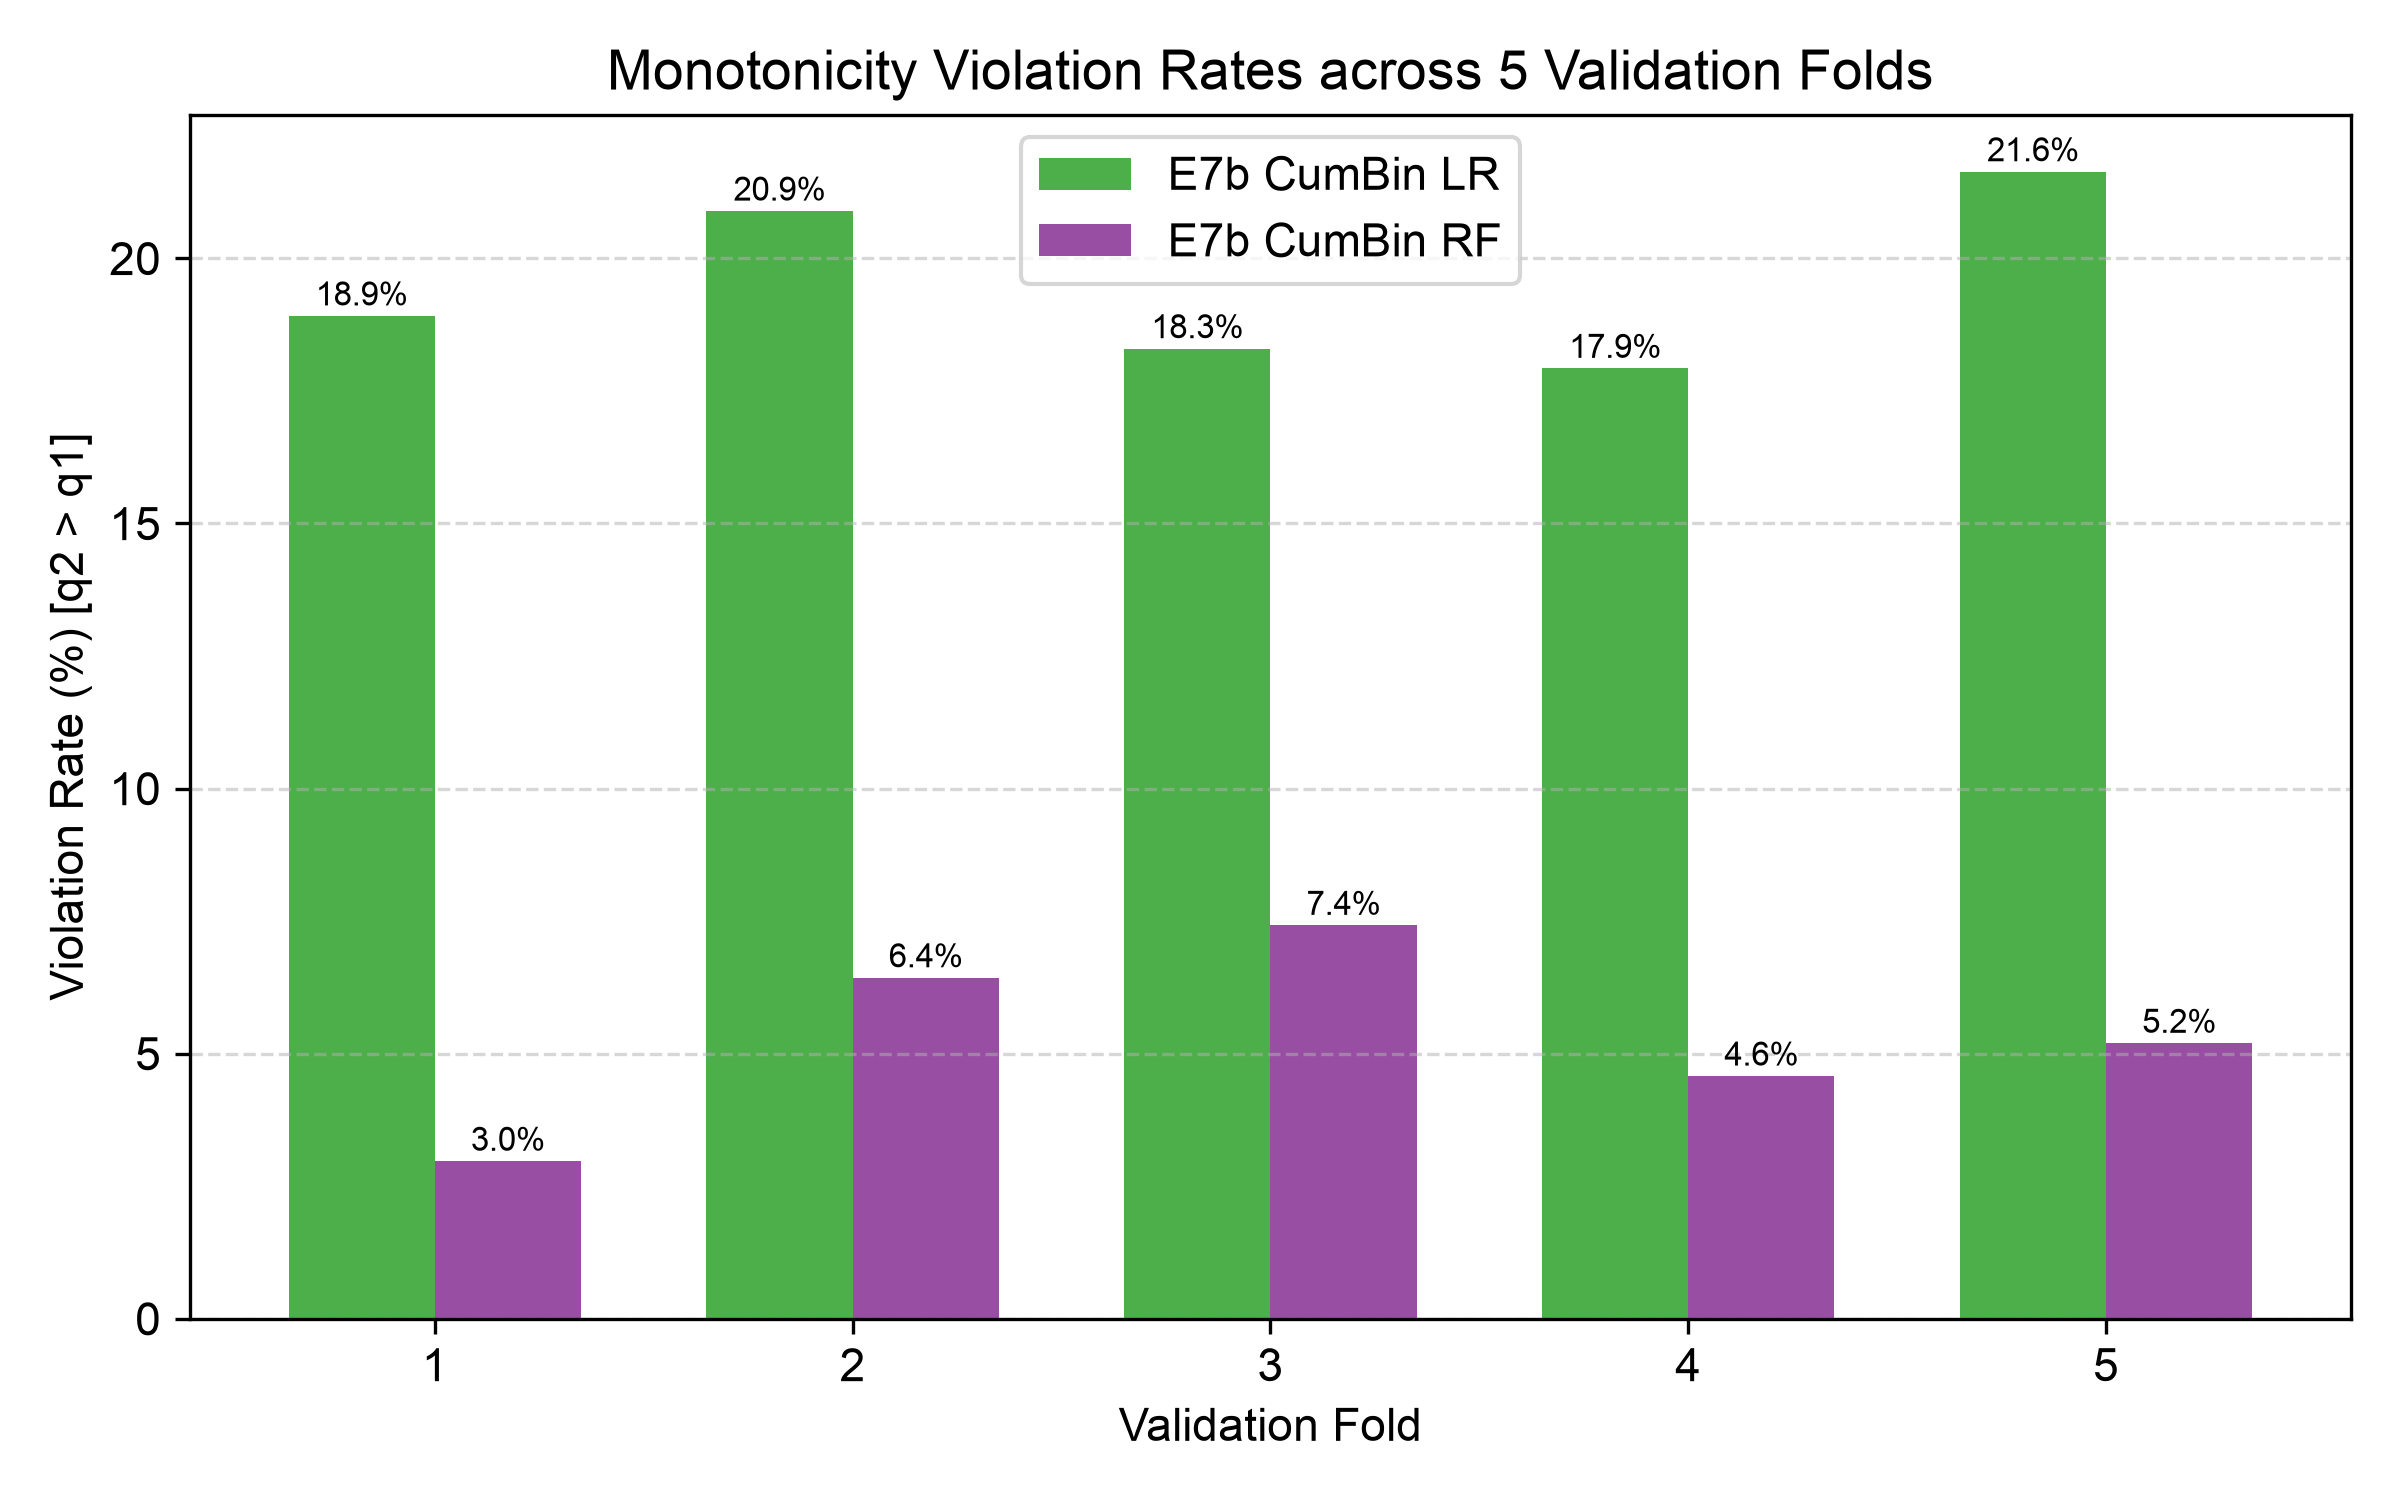
\includegraphics[width=0.75\textwidth]{figures/monotonicity_violation_distribution.png}
\label{fig:monotonicity-violations}
\end{figure}

\textbf{3. Hiệu năng cân bằng của E7a Balanced:}  
Khi tích hợp \texttt{class\_weight="balanced"}, mô hình \texttt{E7a\_Ordinal\_LogReg\_Balanced} duy trì các siêu phẳng song song tuyệt đối (không bao giờ vi phạm đơn điệu), cải thiện đáng kể độ nhạy trên cả ba lớp: Recall $C_0 = 61.24\%$, Recall $C_1 = 32.93\%$, và đạt \textbf{Recall $C_2^+ = 60.37\%$} (cao nhất trong các mô hình cân bằng). Balanced Accuracy đạt mức cao nhất trong toàn bộ nghiên cứu: \textbf{0.5151 $\pm$ 0.0276}.

\subsection{Kết nối phương pháp luận: Tổng kết các trường phái tiếp cận}
Sau khi hoàn thành các khảo sát thực nghiệm riêng lẻ cho từng trường phái — từ phân loại phẳng ($E_0$), phân loại phân cấp cứng ($E_1 \to E_3$), phân cấp mềm nhạy chi phí ($E_4 \to E_6$), đến phân loại thứ bậc ($E_7$) — việc thiết lập một bức tranh đối chiếu toàn diện trên cùng một không gian độ đo đa chiều là bắt buộc để đánh giá khách quan các mối quan hệ đánh đổi lâm sàng. Mục \ref{sec:so-sanh-tong-hop-e0-e7} trình bày bảng tổng hợp chuẩn tắc và các phân tích tương quan sâu sắc.

\FloatBarrier
\section{Bảng so sánh tổng hợp toàn diện (E0 -- E7) trên Legacy Cohort}
\label{sec:so-sanh-tong-hop-e0-e7}

Bảng \ref{tab:master-comparison} tổng hợp toàn bộ 10 mô hình đại diện cho ba trường phái học máy trên cùng tập Legacy Development ($N = 4.045$, Stratified 5-Fold CV cố định). Hình \ref{fig:master-mae-f1} trực quan hóa mối tương quan giữa Macro-F1 và Class MAE, và Hình \ref{fig:master-2step} so sánh chi tiết các lỗi 2 mức nghiêm trọng.

\begin{table}{Bảng so sánh tổng hợp toàn diện các mô hình ($E_0 \to E_7$) trên Legacy Cohort ($N = 4.045$)}
\centering
\footnotesize
\setlength{\tabcolsep}{4pt}
\label{tab:master-comparison}
\begin{tabularx}{\textwidth}{l X c c c c c c c}
\toprule
\textbf{Nhóm} & \textbf{Mô hình} & \textbf{Macro-F1} & \textbf{BalAcc} & \textbf{Acc (\%)} & \textbf{MAE} & \textbf{Rec $C_1$} & \textbf{Rec $C_2^+$} & \textbf{$C_2^+ \to C_0$} \\
\midrule
\textbf{Flat} & $E_0$ (Flat RF) & 0.4354 & 0.4667 & 64.10\% & 0.4638 & 16.29\% & 47.32\% & 108 ca \\
\midrule
\multirow{4}{*}{\textbf{Hard}} 
  & $E_1$ (Hard RF--RF) & 0.4550 & 0.4745 & 68.08\% & 0.4133 & 16.46\% & 43.74\% & 120 ca \\
  & $E_2$ (Hard Tuned)  & \textbf{0.4586} & 0.4745 & 65.32\% & 0.4280 & 25.69\% & 39.63\% & 95 ca \\
  & $E_3a$ (Hard RF--LR)& 0.4567 & 0.4964 & 68.43\% & 0.4195 & 11.75\% & 55.00\% & 120 ca \\
  & $E_3b$ (Hard RF--XGB)& 0.4575 & 0.4790 & 68.23\% & 0.4180 & 16.77\% & 44.76\% & 120 ca \\
\midrule
\multirow{2}{*}{\textbf{Soft}} 
  & $E_4$ (Soft RF--RF) & 0.4206 & 0.4309 & 73.75\% & 0.3530 & 5.18\% & 30.19\% & 227 ca \\
  & $E_5$ (Soft RF--LR) & 0.4270 & 0.4506 & 73.37\% & 0.3619 & 3.45\% & 39.13\% & 211 ca \\
\midrule
\multirow{2}{*}{\textbf{Cost}}
  & $E_{6a}$ (Soft Cost RF--RF) & 0.4535 & 0.4904 & 56.91\% & 0.5216 & \textbf{40.92\%} & 44.25\% & \textbf{62 ca} \\
  & $E_{6b}$ (Soft Cost RF--LR) & 0.4521 & 0.5025 & 56.84\% & 0.5197 & 34.64\% & 54.23\% & \textbf{62 ca} \\
\midrule
\multirow{4}{*}{\textbf{Ordinal}} 
  & $E_{7a}$ (OLR Unweighted)& 0.3846 & 0.4002 & \textbf{75.23\%} & \textbf{0.3377} & 0.00\% & 22.00\% & 305 ca \\
  & $E_{7a}$ (OLR Balanced)  & 0.4518 & \textbf{0.5151} & 56.69\% & 0.5382 & 32.93\% & 60.37\% & 68 ca \\
  & $E_{7b}$ (CumBin LR)     & 0.3761 & 0.4949 & 63.41\% & 0.5718 & 0.00\% & \textbf{72.88\%} & 106 ca \\
  & $E_{7b}$ (CumBin RF)     & 0.4191 & 0.4900 & 72.34\% & 0.3953 & 0.16\% & 57.30\% & 167 ca \\
\midrule
\textbf{Baseline} & Majority Class ($C_0$) & 0.2848 & 0.3333 & 74.56\% & 0.3518 & 0.00\% & 0.00\% & 391 ca \\
\bottomrule
\end{tabularx}
\end{table}


\begin{figure}{Biểu đồ phân tán so sánh Macro-F1 (cao hơn là tốt hơn) và Class MAE (thấp hơn là tốt hơn)}
\centering
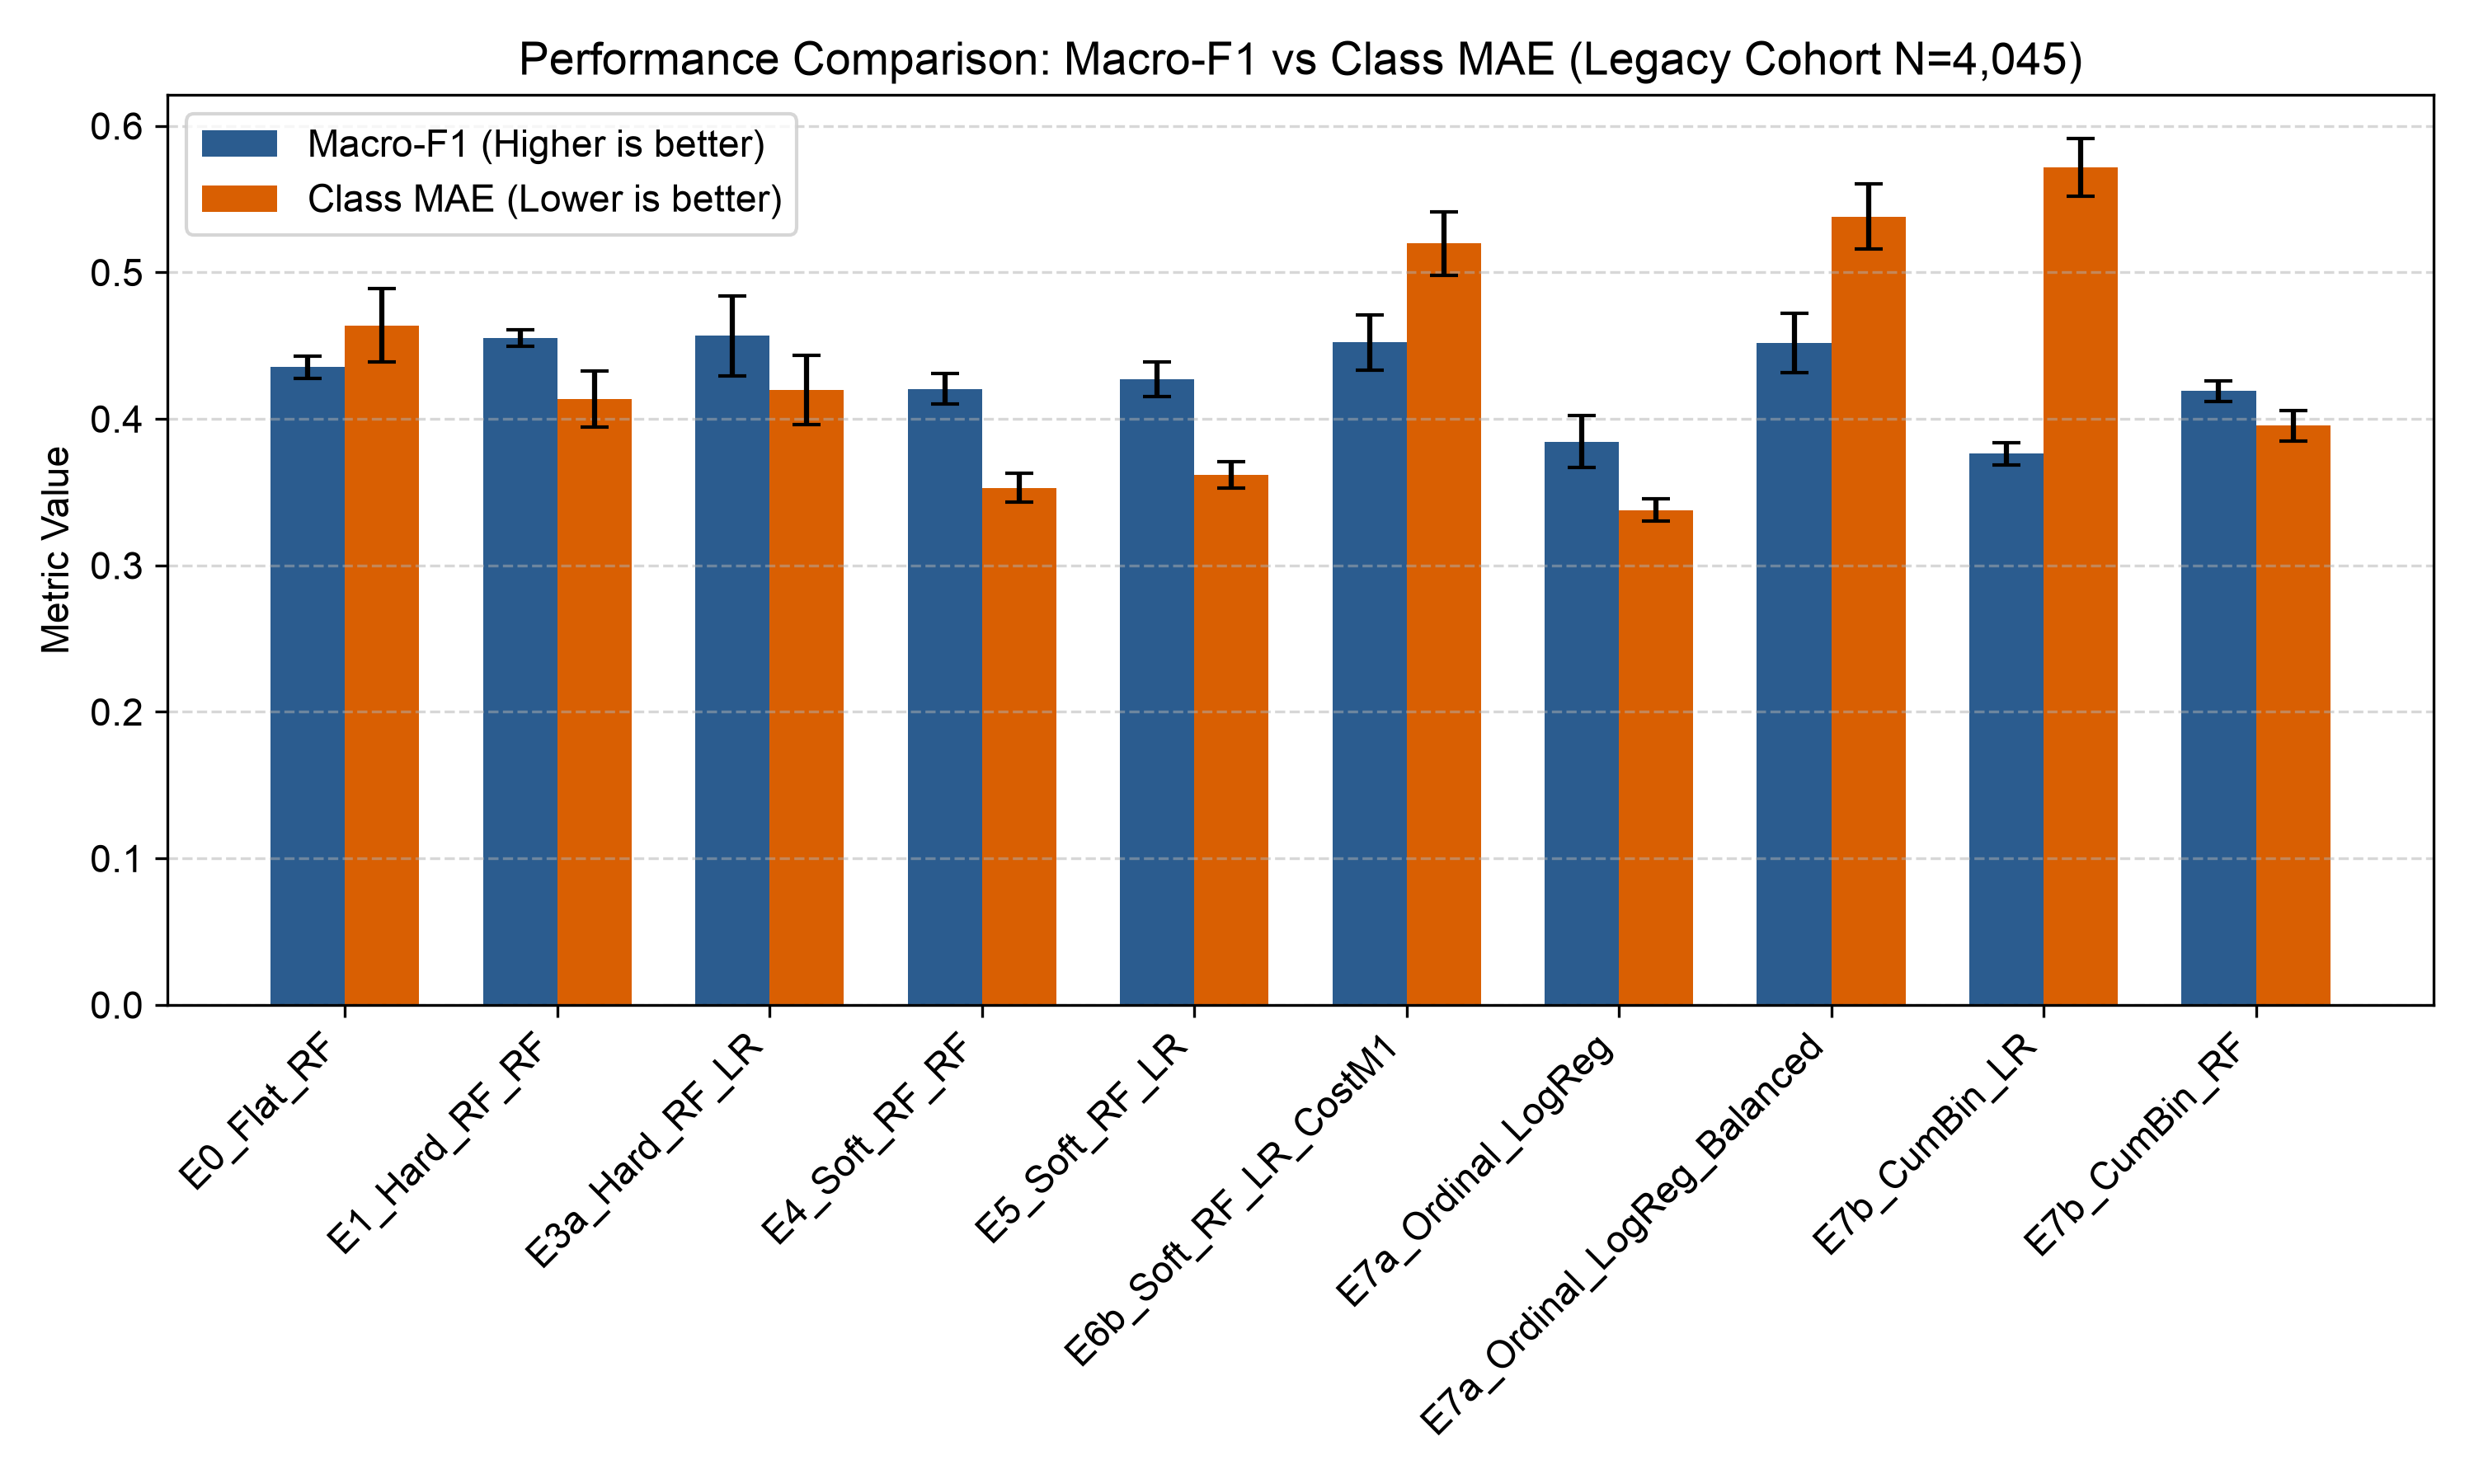
\includegraphics[width=0.88\textwidth]{figures/macro_f1_vs_mae.png}
\label{fig:master-mae-f1}
\end{figure}

\begin{figure}{So sánh số ca sai lệch nghiêm trọng 2 mức: Bỏ sót nặng ($C_2^+ \to C_0$) vs Báo động giả ($C_0 \to C_2^+$)}
\centering
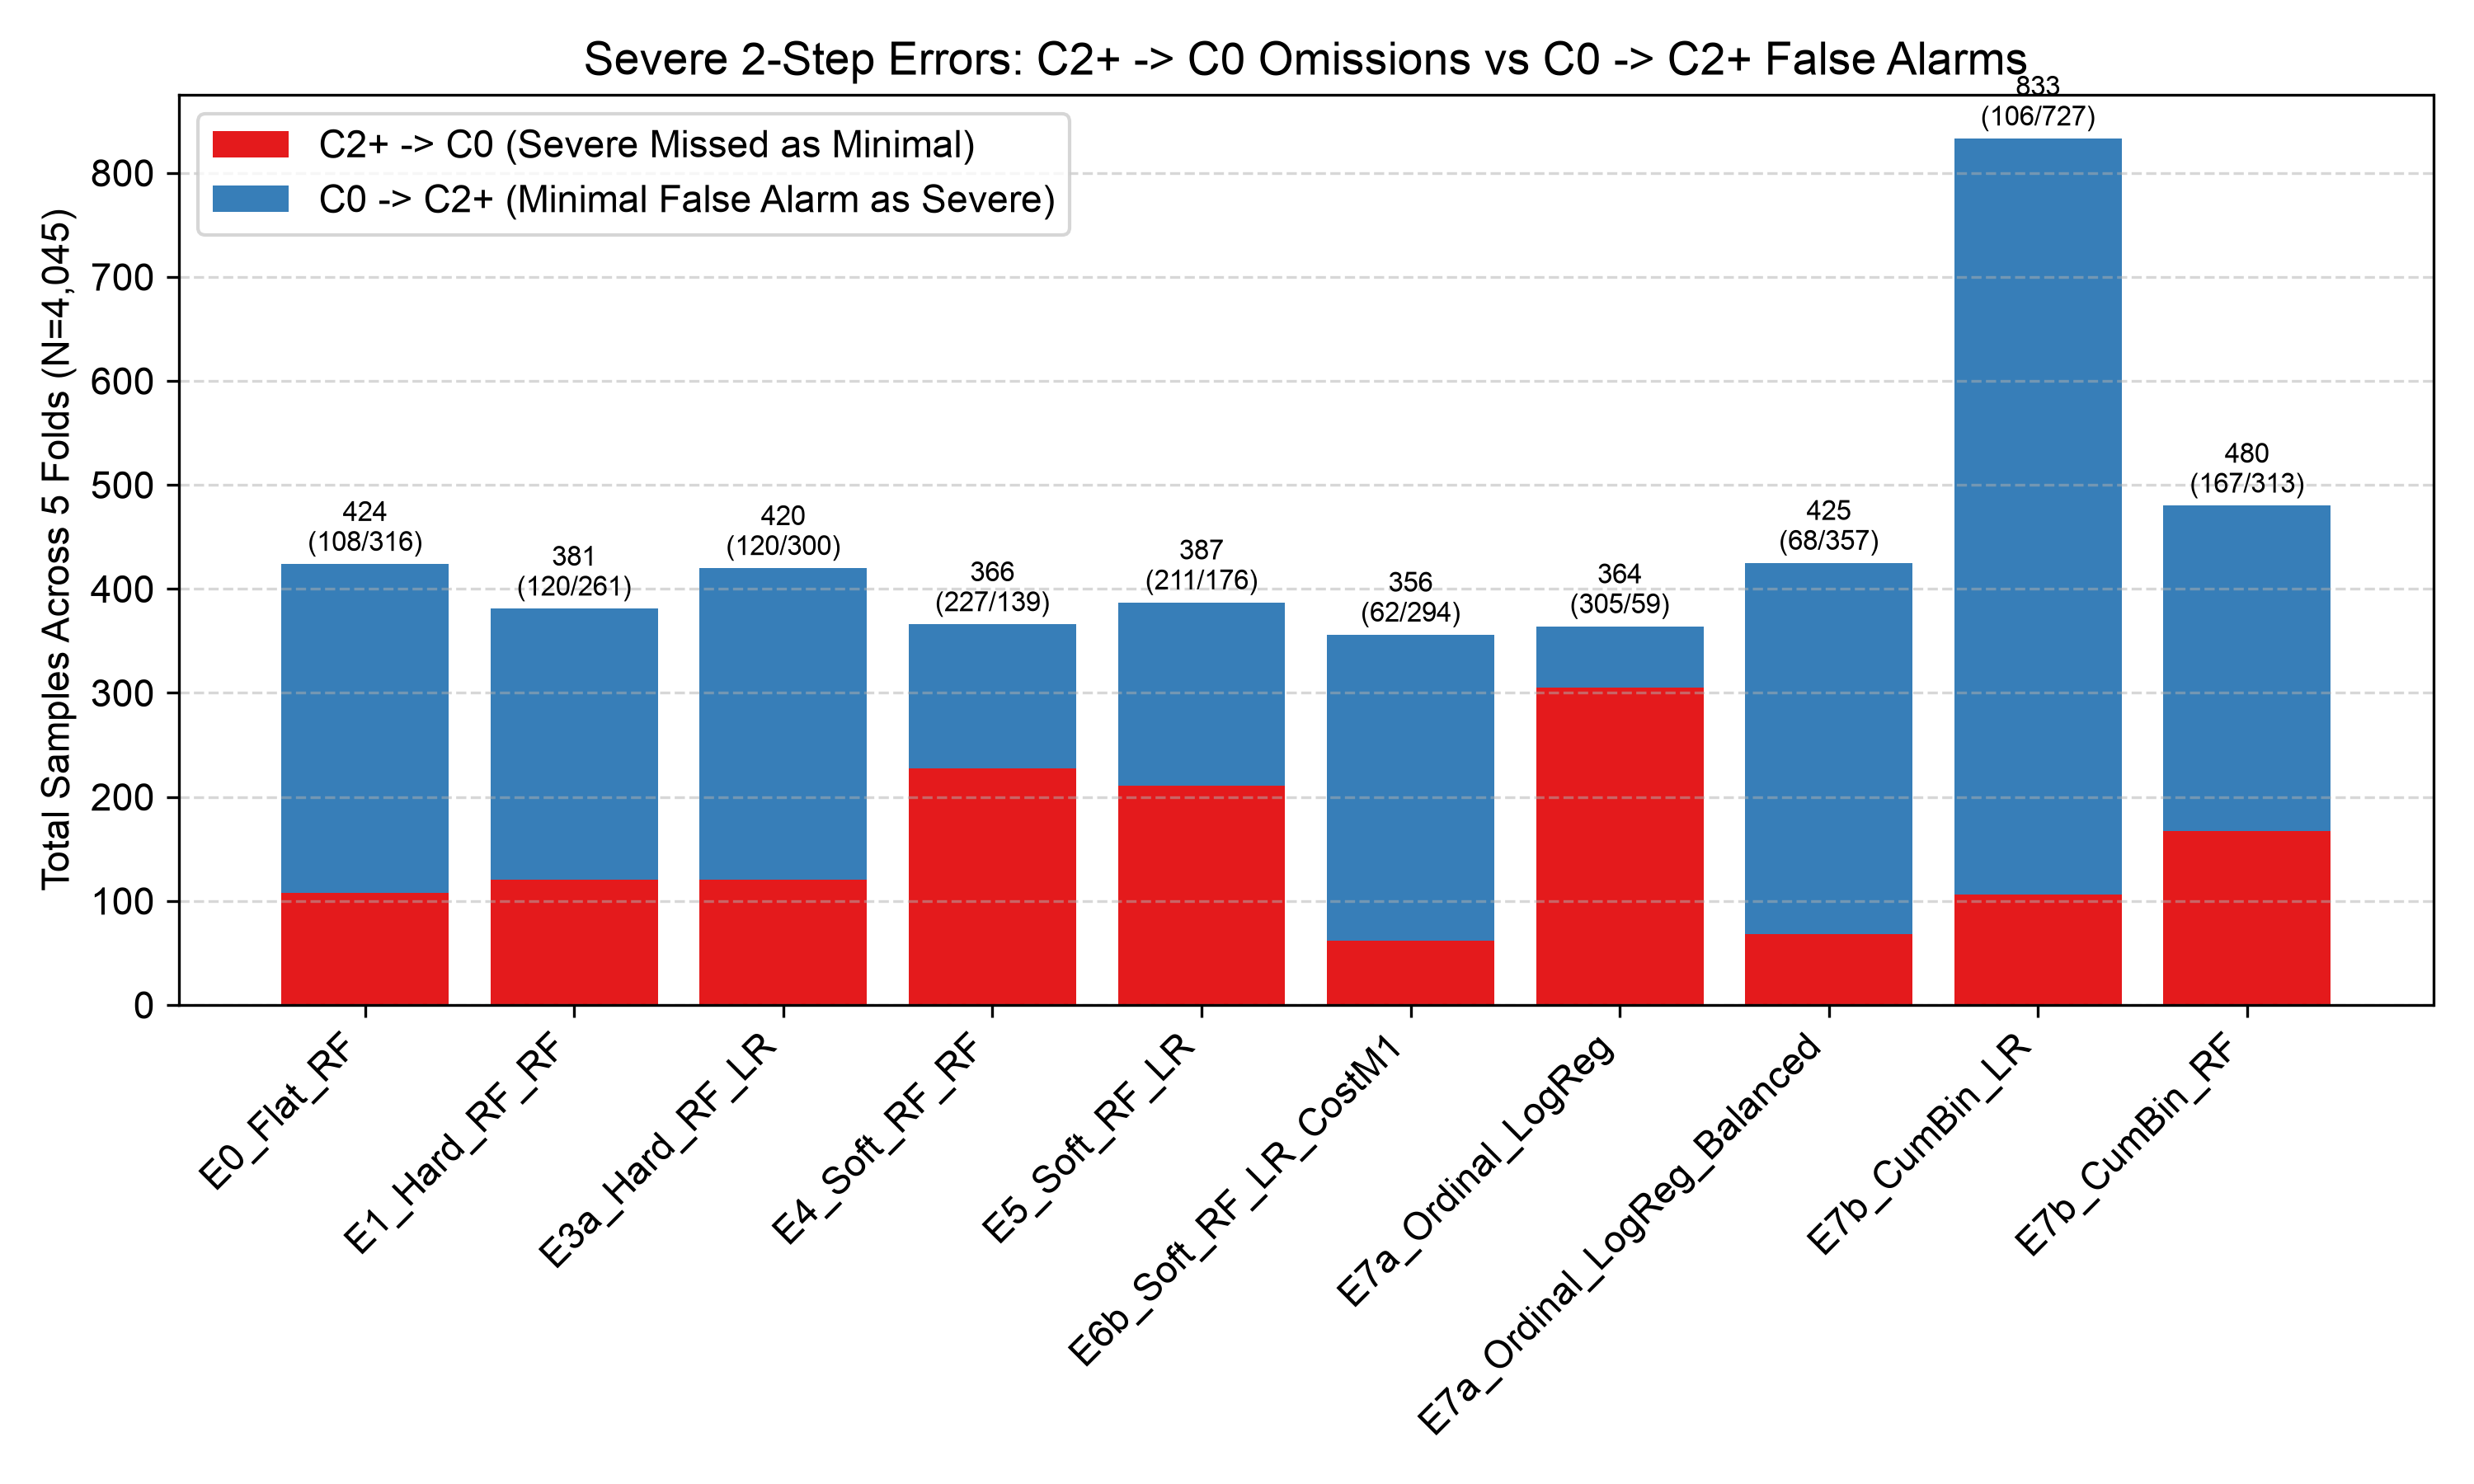
\includegraphics[width=0.88\textwidth]{figures/2step_error_comparison.png}
\label{fig:master-2step}
\end{figure}

\begin{figure}{So sánh ma trận nhầm lẫn Out-of-fold của các mô hình đại diện then chốt trên Legacy Cohort}
\centering
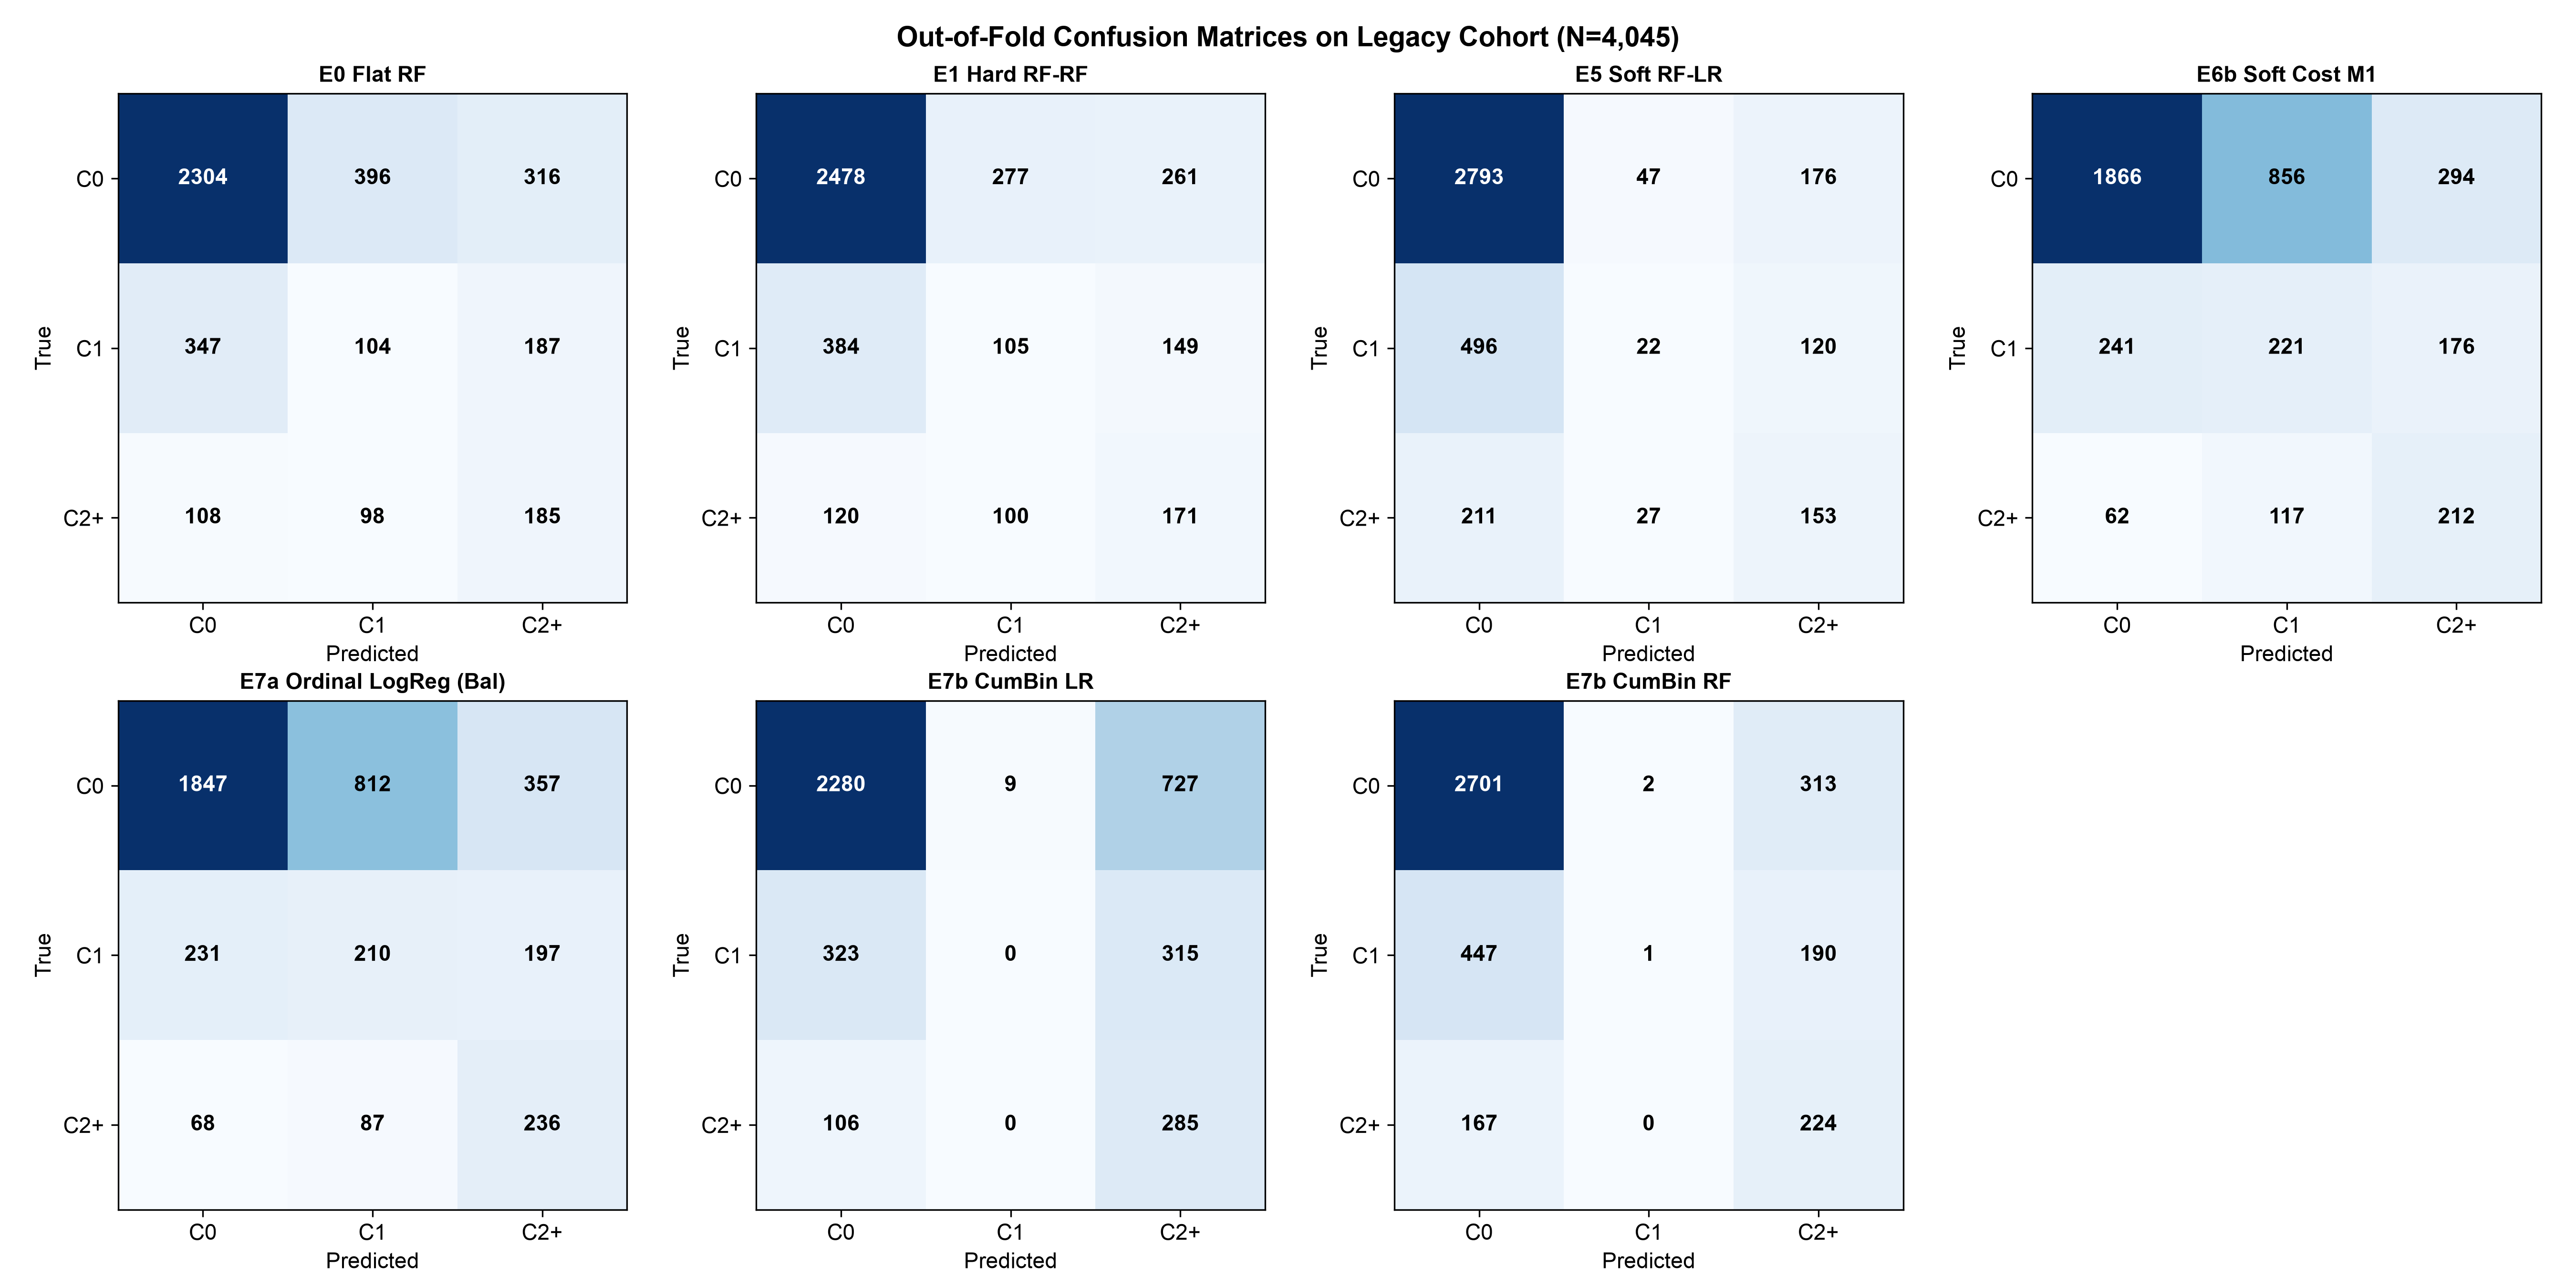
\includegraphics[width=0.95\textwidth]{figures/confusion_matrices_comparison.png}
\label{fig:master-cms}
\end{figure}

\section{Phân tích chuyên sâu về hiệu năng và Đánh giá phản biện}
\label{sec:phan-tich-hieu-nang-thap}

Một câu hỏi cốt lõi mà bất kỳ nhà nghiên cứu hoặc hội đồng phản biện nào cũng sẽ đặt ra khi xem xét kết quả của DepSev-ML:  
\begin{quote}
\textit{“Tại sao các mô hình học máy phức tạp (Ensemble, Hierarchical, Cost-Sensitive, Ordinal) chỉ đạt Macro-F1 trong khoảng $0.43 - 0.46$ và Accuracy chỉ đạt $56\% - 68\%$, trong khi một mô hình ngây thơ (Majority Baseline) dự đoán toàn bộ là $C_0$ có thể đạt Accuracy lên tới $74.56\%$?”}
\end{quote}

Để trả lời câu hỏi này một cách khoa học và thuyết phục, nghiên cứu đưa ra ba luận điểm phân tích thực nghiệm sâu sắc:

\subsection{Sự đánh lừa của chỉ số Accuracy trên dữ liệu mất cân bằng}
Mô hình Majority-Class Baseline gán nhãn dự đoán $\hat{y} = 0$ cho 100\% các quan sát. Trên tập Legacy Development Cohort ($N = 4.045$), mô hình này đạt:
\begin{itemize}
    \item $\text{Accuracy} = 3016 / 4045 = \mathbf{74.56\%}$.
    \item $\text{Macro-F1} = \frac{1}{3} \left( \frac{2 \times 0.7456 \times 1.0}{0.7456 + 1.0} + 0 + 0 \right) = \mathbf{0.2847}$.
    \item $\text{Balanced Accuracy} = \frac{1}{3} (1.0 + 0.0 + 0.0) = \mathbf{0.3333}$.
    \item $\text{Recall } C_1 = \mathbf{0.00\%}$; $\text{Recall } C_2^+ = \mathbf{0.00\%}$.
\end{itemize}

Về mặt ứng dụng y tế, Majority-Class Baseline hoàn toàn \textbf{vô giá trị} vì nó bỏ sót 100\% các ca có triệu chứng trầm cảm ($1.029$ ca bệnh nhân). Nếu một hệ thống y tế chỉ nhìn vào Accuracy để đánh giá, nó sẽ ưu tiên chọn một mô hình không có khả năng phát hiện bệnh!

Ngược lại, mô hình \texttt{E7a\_Ordinal\_LogReg\_Balanced} dù có Accuracy là $56.69\%$ (thấp hơn 74.56\%), nhưng đạt \textbf{Balanced Accuracy = 51.51\%} (cao hơn 33.33\% tới +18.2\%) và nhận diện được \textbf{60.37\% các ca bệnh nặng} ($C_2^+$) cùng \textbf{32.93\% các ca nhẹ} ($C_1$). Đây chính là giá trị thực tiễn đích thực của học máy có kiểm soát.

\subsection{Bản chất sinh học của hiện tượng chồng lấn đặc trưng (Feature Overlap)}
Trầm cảm là một hội chứng tâm thần kinh phức tạp có căn nguyên đa yếu tố (gen di truyền, sang chấn tâm lý xã hội, môi trường sống, sự mất cân bằng chất dẫn truyền thần kinh Serotonin/Dopamine trong não bộ). Các chỉ số sinh lý ngoại vi (như huyết áp, men gan, mỡ máu, chỉ số đường huyết) chỉ phản ánh các biến đổi chuyển hóa gián tiếp đi kèm. 

Hiện tượng diện tích chồng lấn Bayes $\Omega_{\text{overlap}}$ giữa người bình thường ($C_0$) và người trầm cảm nhẹ ($C_1$) rất lớn (Hình \ref{fig:overlap-pca}) tạo nên một rào cản hiệu năng đối với các bộ phân loại hiện tại trong khoảng Macro-F1 từ $0.45$ đến $0.46$. Trong giới hạn của các biến số sinh lý ngoại vi và xét nghiệm máu thường quy hiện có trong NHANES, việc nâng cao hơn nữa hiệu năng phân tách đòi hỏi phải bổ sung các chiều dữ liệu y sinh chuyên sâu hơn (như các chỉ dấu phân tử sinh học, hormone căng thẳng Cortisol hoặc dữ liệu theo dõi hành vi liên tục từ thiết bị đeo).

\subsection{Bản đồ đánh đổi và tính không thể thay thế tuyệt đối}
Thực nghiệm khẳng định không có một mô hình nào là tối ưu toàn diện trên mọi thước đo:
\begin{itemize}
    \item Nếu ưu tiên \textbf{Accuracy cao nhất và MAE thấp nhất}: Chọn \texttt{E7a Unweighted} (Acc 75.23\%, MAE 0.3377), nhưng phải chấp nhận mất hoàn toàn nhóm nhẹ $C_1$.
    \item Nếu ưu tiên \textbf{Macro-F1 cao nhất}: Chọn \texttt{E2} (Macro-F1 0.4586) hoặc \texttt{E3a} (0.4567), nhưng phải chấp nhận 120 ca nặng bị tắc nghẽn ở Giai đoạn 1.
    \item Nếu ưu tiên \textbf{An toàn lâm sàng, giảm thiểu tối đa ca bỏ sót nặng}: Chọn \texttt{E6b} (chỉ bỏ sót 62 ca $C_2^+ \to C_0$).
    \item Nếu ưu tiên \textbf{Cân bằng đa lớp toàn diện và nhận diện ca nặng tốt nhất}: Chọn \texttt{E7a\_Ordinal\_LogReg\_Balanced} (Balanced Accuracy 0.5151, Recall $C_2^+ = 60.37\%$).
\end{itemize}

\section{Thảo luận và Trả lời các câu hỏi nghiên cứu}
\label{sec:thao-luan-rq}

\begin{itemize}
    \item \textbf{Trả lời RQ1:} Nhóm xét nghiệm cận lâm sàng máu ($F_2$) và lối sống ($F_3$) đóng góp thực chất nhất vào mức tăng hiệu năng (+14\% đến +23\% Macro-F1 so với chỉ dùng dấu hiệu sinh tồn $F_1$). Việc kết hợp toàn diện $F_4$ mang lại lợi thế lớn nhất khi mô hình được tinh chỉnh siêu tham số có kiểm soát.
    \item \textbf{Trả lời RQ2:} Hiệu năng suy giảm mạnh nhất tại bước chuyển $T_2 \to T_3$ (Macro-F1 giảm 34.4\%), với điểm nghẽn tập trung tại ranh giới phân tách lớp nhẹ $C_1$ do sự chồng lấn phân phối sinh lý với lớp bình thường $C_0$.
    \item \textbf{Trả lời RQ3:} Mở rộng dữ liệu lên 3 chu kỳ NHANES ($N = 14.581$) giúp ổn định phân phối của các lớp hiếm $C_3/C_4$, nhưng không giúp cải thiện Macro-F1 tổng thể do trần chồng lấn đặc trưng.
    \item \textbf{Trả lời RQ4:} Phân loại phân cấp hai tầng cứng cải thiện nhẹ Macro-F1 (+0.02 so với Flat RF) nhưng gây ra hiện tượng lan truyền sai số nghiêm trọng khi loại bỏ nhầm 30.7\% số ca bệnh nặng ở Giai đoạn 1.
    \item \textbf{Trả lời RQ5:} Mô hình Soft Hierarchical nhạy chi phí ($E_{6a}, E_{6b}$) và Ordinal Logistic Regression cân bằng ($E_{7a}$) đã khắc phục hiệu quả sự tắc nghẽn của cổng cứng, giảm số ca bỏ sót nặng $C_2^+ \to C_0$ từ 120 ca xuống còn 62--68 ca, nâng Balanced Accuracy lên mức cao nhất 0.5151 và duy trì độ ổn định trên tập kiểm tra theo dòng thời gian (Branch D, Balanced Accuracy = 0.5073).
\end{itemize}
\cleardoublepage

\chapter{Kết luận và hướng phát triển}
\label{ch:ket-luan}

\section{Kết quả đạt được}
\label{sec:ket-qua-dat-duoc}

Công trình nghiên cứu \textbf{“Nghiên cứu khung học máy cho dự đoán mức độ triệu chứng trầm cảm từ dữ liệu sinh lý (DepSev-ML)”} đã thực hiện một khảo sát toàn diện, có hệ thống và nghiêm ngặt về mặt phương pháp luận đối với bài toán lượng giá mức độ nghiêm trọng của triệu chứng trầm cảm PHQ-9 từ các đặc trưng sinh lý dạng bảng. 

Qua các giai đoạn thực nghiệm có kiểm soát chặt chẽ, đề tài đã đạt được các kết quả cụ thể:
\begin{enumerate}
    \item \textbf{Khảo sát cắt bỏ đặc trưng và tinh chỉnh mô hình nền tảng:} Xác lập được vai trò then chốt của việc kết hợp các chỉ số cận lâm sàng máu thiết yếu cùng tiền sử bệnh lý mạn tính lâm sàng ($F_2$) và hành vi sinh hoạt ($F_3$), giúp tăng từ +14\% đến +23\% Macro-F1 so với chỉ sử dụng các dấu hiệu thể chất và sinh tồn ngoại vi đơn lẻ. Thông qua quy trình Nested CV khắt khe, mô hình \texttt{Random Forest/F4} với siêu tham số tối ưu đã được lựa chọn làm xương sống chuẩn mực cho toàn bộ hệ thống.
    \item \textbf{Lượng hóa quy luật suy giảm hiệu năng theo độ chi tiết nhãn ($T_2 \to T_5$):} Lần đầu tiên lượng hóa chính xác sự sụt giảm hiệu năng khi tăng số lượng lớp dự đoán: Macro-F1 giảm từ 0.6639 ($T_2$) xuống 0.4354 ($T_3$), 0.3380 ($T_4$) và 0.2630 ($T_5$). Nghiên cứu chứng minh bằng thực nghiệm và phân tích PCA rằng bước chuyển $T_2 \to T_3$ là điểm suy giảm lớn nhất do sự chồng lấn phân phối sinh lý dày đặc giữa nhóm người bình thường ($C_0$) và nhóm có triệu chứng nhẹ ($C_1$).
    \item \textbf{Đánh giá tổng quát hóa trên dữ liệu đa chu kỳ quy mô lớn ($N = 14.581$):} Thực hiện quy trình hài hòa hóa dữ liệu chuẩn xác trên 3 chu kỳ NHANES liên tiếp với bộ đặc trưng $F_{4\_\text{common31}}$ gồm 31 biến số. Kết quả thực nghiệm đối chứng khẳng định việc tăng cỡ mẫu lên gấp 3 lần giúp ổn định độ nhạy của các lớp hiếm ($C_3, C_4$), nhưng không thể tự động đảo ngược hoàn toàn trần hiệu năng Macro-F1 của bài toán phân loại đa mức chi tiết nếu không có sự mở rộng về không gian đặc trưng.
    \item \textbf{Phân tích bản chất và khắc phục Error Propagation trong Phân loại phân cấp:} Chỉ ra khiếm khuyết lâm sàng của kiến trúc Hard Hierarchical ($E_1$) khi cơ chế cổng nhị phân cứng loại bỏ nhầm tới 120 bệnh nhân nặng quy ước ($C_2^+$) ở Giai đoạn 1. Đề xuất thành công mô hình Soft Probability Fusion kết hợp tối ưu chi phí Bayes ($E_{6a}, E_{6b}$), kéo giảm số ca bỏ sót $C_2^+ \to C_0$ từ 120 ca xuống chỉ còn 62 ca (giảm 48.3\%).
    \item \textbf{Hiệu quả vượt trội của mô hình Phân loại thứ bậc cân bằng ($E_7a$):} Hiện thực mô hình Ordinal Logistic Regression (Proportional Odds) với ràng buộc tái tham số hóa số mũ, bảo đảm tính đơn điệu tuyệt đối của các ngưỡng cắt. Mô hình \texttt{E7a\_Ordinal\_LogReg\_Balanced} đạt mức cao nhất toàn dự án về \textbf{Balanced Accuracy = 0.5151} trên Legacy Cohort và duy trì \textbf{0.5073} trên tập kiểm tra độc lập theo dòng thời gian (Branch D, $N = 4.888$), nâng độ nhạy nhận diện nhóm nặng $C_2^+$ lên mức \textbf{60.37\%}. Đồng thời, nghiên cứu cũng chỉ ra hạn chế của phương pháp Frank \& Hall ($E_7b$) khi ghi nhận tới 19.53\% số mẫu vi phạm tính đơn điệu.
\end{enumerate}

\section{Đóng góp nghiên cứu}
\label{sec:dong-gop-khoa-hoc}

Công trình mang lại những đóng góp khoa học và thực tiễn rõ nét cho lĩnh vực Tin sinh học và Học máy y tế:
\begin{enumerate}
    \item \textbf{Đóng góp về phương pháp luận kiểm định liêm chính (Strict Zero Leakage Methodology):} Xây dựng một quy trình chuẩn tắc khép kín, phân tách minh bạch giữa tập phát triển và tập kiểm tra, mã hóa toàn bộ đường ống tiền xử lý bên trong từng fold, loại bỏ hoàn toàn các biến mục tiêu DPQ khỏi ma trận đặc trưng, tạo nên một chuẩn mực thực nghiệm có độ tin cậy và khả năng tái lập cao.
    \item \textbf{Tài sản dữ liệu chuẩn hóa (Harmonized Multi-cycle Dataset):} Hoàn thiện bộ dữ liệu chuẩn hóa $F_{4\_\text{common31}}$ trên gần 15.000 đối tượng qua 3 chu kỳ NHANES, giải quyết vấn đề không đồng nhất schema và cung cấp mã nguồn mở phục vụ cho các nghiên cứu tiếp theo về sức khỏe tâm thần dạng bảng.
    \item \textbf{Làm sáng tỏ bản chất của bài toán phân tầng rủi ro trầm cảm:} Khẳng định bằng dữ liệu thực nghiệm rằng bài toán dự đoán trầm cảm từ dữ liệu sinh lý không thể chỉ nhìn vào độ chính xác Accuracy bề nổi. Nghiên cứu cung cấp một bức tranh toàn diện về các mối quan hệ đánh đổi giữa Macro-F1, Balanced Accuracy, Class MAE và sự an toàn lâm sàng (giảm thiểu bỏ sót ca bệnh nặng).
    \item \textbf{Giải pháp kiến trúc kết hợp tối ưu:} Đề xuất thành công hai giải pháp kiến trúc có giá trị ứng dụng thực tế cao: mô hình Soft Cost-Sensitive ($E_6b$) cho các bài toán yêu cầu phạt nặng ca bỏ sót, và mô hình Ordinal Logistic Regression cân bằng ($E_7a$) cho các bài toán yêu cầu cân bằng độ nhạy đa mức độ và tôn trọng thứ tự nghiêm ngặt của bệnh học.
\end{enumerate}

\section{Hạn chế khoa học}
\label{sec:han-che-khoa-hoc}

Bên cạnh những kết quả đạt được, nghiên cứu cũng thẳng thắn thừa nhận các hạn chế khoa học mang tính khách quan:
\begin{enumerate}
    \item \textbf{Trần hiệu năng của dữ liệu sinh lý ngoại vi:} Bản thân thang đo PHQ-9 là công cụ tự báo cáo phản ánh trạng thái cảm xúc và nhận thức chủ quan. Các chỉ số sinh lý đo lường ở ngoại vi (huyết áp, nhân trắc, xét nghiệm máu thông thường) chỉ phản ánh các tương quan chuyển hóa gián tiếp, do đó tồn tại một "trần hiệu năng" tự nhiên đối với Macro-F1 quanh mức 0.45 -- 0.46 trên không gian 3 lớp và 0.26 -- 0.27 trên không gian 5 lớp.
    \item \textbf{Giới hạn của thiết kế khảo sát cắt ngang (Cross-Sectional Design):} Dữ liệu NHANES thu thập các chỉ số tại một thời điểm duy nhất trong phòng khám lưu động. Nghiên cứu không có dữ liệu theo dõi dọc (longitudinal data) theo thời gian của từng cá nhân, do đó không thể theo dõi diễn tiến dao động triệu chứng của bệnh nhân.
    \item \textbf{Sự đánh đổi về cảnh báo giả (False Positives):} Để đạt được độ nhạy trên 60\% đối với nhóm nặng $C_2^+$, mô hình \texttt{E7a\_Balanced} phải chấp nhận tỷ lệ báo động nhầm $C_0 \to C_2^+$ là 11.8\% (357 ca). Trong các chiến dịch tầm soát cộng đồng, điều này có thể làm tăng gánh nặng chi phí cho các xét nghiệm khẳng định tiếp theo.
    \item \textbf{Giả định tuyến tính trong mô hình Proportional Odds:} Mô hình \texttt{E7a} hiện tại giả định quan hệ tuyến tính giữa biến tiềm ẩn và các đặc trưng đầu vào, chưa khai thác được các tương tác phi tuyến bậc cao phức tạp như các mô hình dựa trên cây quyết định.
    \item \textbf{Thiết kế khảo sát phức hợp chưa có trọng số (Complex Survey Sampling):} Các mô hình được tối ưu hóa theo rủi ro thực nghiệm không trọng số (Unweighted ERM) theo chuẩn benchmark học máy thông thường, chưa tích hợp hàm hợp lý giả có trọng số lấy mẫu (\texttt{WTINT2YR}, \texttt{WTMEC2YR}) để suy luận dịch tễ học cấp độ toàn dân số Hoa Kỳ.
\end{enumerate}

\section{Hướng phát triển tiếp theo}
\label{sec:huong-phat-trien}

Dựa trên các phát hiện thực nghiệm và các hạn chế đã xác định, những hướng nghiên cứu có cơ sở khoa học vững chắc và cần được ưu tiên triển khai trong tương lai bao gồm:
\begin{enumerate}
    \item \textbf{Phát triển Rừng cây tăng cường thứ bậc phi tuyến (Non-linear Ordinal Gradient Boosting):} Tích hợp hàm mất mát Cumulative Logit Loss hoặc Proportional Odds Loss trực tiếp vào thuật toán phân chia nhánh của XGBoost và LightGBM. Hướng đi này hứa hẹn sẽ kết hợp hoàn hảo ưu thế bảo đảm tính thứ bậc và không vi phạm đơn điệu của $E_7a$ với khả năng học tương tác phi tuyến cực mạnh của cây quyết định.
    \item \textbf{Huấn luyện nhị phân có ràng buộc đơn điệu đồng thời (Constrained Joint Multi-task Training):} Cải tiến phương pháp Frank \& Hall bằng cách đưa số hạng phạt vi phạm đơn điệu $L_{\text{monotonicity}} = \lambda \sum \max(0, q_2(\mathbf{x}) - q_1(\mathbf{x}))^2$ trực tiếp vào hàm mục tiêu huấn luyện chung (Joint Loss) của mạng nơ-ron đa nhiệm (Multi-task Neural Network), triệt tiêu hiện tượng giao cắt siêu phẳng ngay từ khâu học trọng số.
    \item \textbf{Tích hợp các chỉ dấu sinh học sâu hơn (Deep Molecular Biomarkers):} Mở rộng không gian đặc trưng bằng cách tích hợp thêm các dữ liệu chuyên biệt về nồng độ hormone căng thẳng (Cortisol huyết thanh hoặc nước bọt), các chỉ số viêm mạn tính chuyên sâu (chỉ số protein phản ứng C độ nhạy cao -- hs-CRP, Interleukin-6), và các biến thể di truyền (genetic polymorphisms) khi nguồn dữ liệu cho phép.
    \item \textbf{Khai thác dữ liệu cảm biến đeo liên tục (Wearable Sensor Data):} Kết hợp các chỉ số xét nghiệm tĩnh với dữ liệu đo lường liên tục trong đời sống hàng ngày thu nhận từ đồng hồ thông minh hoặc thiết bị đeo (biến thiên nhịp tim HRV, chất lượng giấc ngủ vi mô, nhịp sinh học ngày đêm), hướng tới một hệ sinh thái chăm sóc sức khỏe tâm thần chủ động và cá nhân hóa cao độ.
\end{enumerate}
\cleardoublepage


% ==================== DANH MỤC TÀI LIỆU THAM KHẢO ====================
\begin{thebibliography}{99}

\begin{bibsection}{Tài liệu tham khảo tiếng Việt}
\bibitem{byt2020}
    Bộ Y tế,
    \textit{Hướng dẫn chẩn đoán và điều trị các rối loạn trầm cảm},
    Nhà xuất bản Y học, Hà Nội, 2020.
\end{bibsection}

\begin{bibsection}{Tài liệu tham khảo tiếng Anh}
\bibitem{kroenke2001phq}
    K. Kroenke, R. L. Spitzer, and J. B. Williams,
    ``The {PHQ-9}: Validity of a brief depression severity measure,''
    \textit{Journal of General Internal Medicine}, vol. 16, no. 9, pp. 606--613, 2001.

\bibitem{spitzer1999validation}
    R. L. Spitzer, K. Kroenke, and J. B. Williams,
    ``Validation and utility of a self-report version of {PRIME-MD}: The {PHQ} primary care study,''
    \textit{JAMA}, vol. 282, no. 18, pp. 1737--1744, 1999.

\bibitem{breiman2001random}
    L. Breiman,
    ``Random Forests,''
    \textit{Machine Learning}, vol. 45, no. 1, pp. 5--32, 2001.

\bibitem{chen2016xgboost}
    T. Chen and C. Guestrin,
    ``{XGBoost}: A scalable tree boosting system,''
    in \textit{Proceedings of the 22nd ACM SIGKDD International Conference on Knowledge Discovery and Data Mining}, pp. 785--794, 2016.

\bibitem{mccullagh1980regression}
    P. McCullagh,
    ``Regression models for ordinal data,''
    \textit{Journal of the Royal Statistical Society: Series B (Methodological)}, vol. 42, no. 2, pp. 109--127, 1980.

\bibitem{frank2001simple}
    E. Frank and M. Hall,
    ``A simple approach to ordinal classification,''
    in \textit{Proceedings of the 12th European Conference on Machine Learning (ECML)}, pp. 145--156, 2001.

\bibitem{elkan2001foundations}
    C. Elkan,
    ``The foundations of cost-sensitive learning,''
    in \textit{Proceedings of the 17th International Joint Conference on Artificial Intelligence (IJCAI)}, vol. 17, pp. 973--978, 2001.

\bibitem{he2009learning}
    H. He and E. A. Garcia,
    ``Learning from imbalanced data,''
    \textit{IEEE Transactions on Knowledge and Data Engineering}, vol. 21, no. 9, pp. 1263--1284, 2009.

\bibitem{chawla2002smote}
    N. V. Chawla, K. W. Bowyer, L. O. Hall, and W. P. Kegelmeyer,
    ``{SMOTE}: Synthetic minority over-sampling technique,''
    \textit{Journal of Artificial Intelligence Research}, vol. 16, pp. 321--357, 2002.

\bibitem{cdc2014nhanes}
    Centers for Disease Control and Prevention (CDC),
    \textit{National Health and Nutrition Examination Survey: 2013-2014 Data Documentation, Codebook, and Frequencies},
    National Center for Health Statistics (NCHS), Hyattsville, MD, 2014.

\bibitem{cdc2016nhanes}
    Centers for Disease Control and Prevention (CDC),
    \textit{National Health and Nutrition Examination Survey: 2015-2016 Overview and Analytic Guidelines},
    National Center for Health Statistics (NCHS), Hyattsville, MD, 2016.

\bibitem{lundberg2017unified}
    S. M. Lundberg and S.-I. Lee,
    ``A unified approach to interpreting model predictions,''
    \textit{Advances in Neural Information Processing Systems}, vol. 30, pp. 4765--4774, 2017.

\bibitem{silla2011survey}
    C. N. Silla and A. A. Freitas,
    ``A survey of hierarchical classification across different application domains,''
    \textit{Data Mining and Knowledge Discovery}, vol. 22, no. 1, pp. 31--72, 2011.

\bibitem{pedregosa2011scikit}
    F. Pedregosa, G. Varoquaux, A. Gramfort, V. Michel, B. Thirion, O. Grisel, M. Blondel, P. Prettenhofer, R. Weiss, V. Dubourg, et al.,
    ``Scikit-learn: Machine learning in Python,''
    \textit{Journal of Machine Learning Research}, vol. 12, pp. 2825--2830, 2011.

\bibitem{cohen1968weighted}
    J. Cohen,
    ``Weighted chi-square: An extension of the kappa coefficient for nominal scales with unequal disagreement weights,''
    \textit{Psychological Bulletin}, vol. 70, no. 4, pp. 213--220, 1968.

\bibitem{wolpert1992stacked}
    D. H. Wolpert,
    ``Stacked generalization,''
    \textit{Neural Networks}, vol. 5, no. 2, pp. 241--259, 1992.

\bibitem{varma2006bias}
    S. Varma and R. Simon,
    ``Bias in error estimation when using cross-validation for model selection,''
    \textit{BMC Bioinformatics}, vol. 7, no. 1, p. 91, 2006.

\bibitem{platt1999probabilistic}
    J. Platt,
    ``Probabilistic outputs for support vector machines and comparisons to regularized likelihood methods,''
    \textit{Advances in Large Margin Classifiers}, vol. 10, no. 3, pp. 61--74, 1999.

\bibitem{zadrozny2002transforming}
    B. Zadrozny and C. Elkan,
    ``Transforming classifier scores into accurate multiclass probability estimates,''
    in \textit{Proceedings of the Eighth ACM SIGKDD International Conference on Knowledge Discovery and Data Mining}, pp. 694--699, 2002.

\bibitem{pratt1991discriminant}
    L. A. Pratt, D. J. Brody, and Q. Gu,
    ``Depression in the {U.S.} household population, 2009--2012,''
    \textit{NCHS Data Brief}, no. 172, pp. 1--8, 2014.
\end{bibsection}

\end{thebibliography}

\end{document}
